\documentclass[specialist,
               substylefile = spbu.rtx,
               subf,href,colorlinks=true, 12pt]{disser}

\usepackage[a4paper,
            mag=1000, includefoot,
            left=3cm, right=1.5cm, top=2cm, bottom=2cm, headsep=1cm, footskip=1cm]{geometry}
\usepackage[T2A]{fontenc}
\usepackage[utf8]{inputenc}
\usepackage[english,russian]{babel}
\usepackage{graphicx}
\usepackage{multicol,caption}
\usepackage{multirow}
\usepackage{amsfonts}
\usepackage{amsmath}
\usepackage{amssymb}
\usepackage[noabbrev]{cleveref}
\usepackage{makecell}
\newcommand{\R}{\mathbb{R}}
\def\RE{\mathop{\mathrm{Re}}}
\def\VAR{\mathop{\mathrm{var}}}
\def\rank{\mathop{\mathrm{rank}}}
\def\mod{\mathop{\mathrm{mod}}}
\def\argmin{\mathop{\mathrm{argmin}}}
\def\argmax{\mathop{\mathrm{argmax}}}
\def\mean{\mathop{\mathrm{mean}}}
\def\IM{\mathop{\mathrm{Im}}}
\def\vec{\mathop{\mathrm{vec}}}
\def\matr{\mathop{\mathrm{matr}}}
\def\Span{\mathop{\mathrm{span}}}
\def\cov{\mathop{\mathrm{cov}}}
\def\Span{\mathop{\mathrm{span}}}
\def\corr{\mathop{\mathrm{corr}}}
\DeclareMathOperator{\Real}{\mathbb{R}}
\DeclareMathOperator{\D}{\mathbb{D}}
\newcommand{\I}{\mathrm{i}}

\makeatother
\newcommand{\pkg}[1]{\textsc{#1}}
\let\proglang=\textsf
\usepackage{xspace}
\def\R{{\normalfont\ttfamily R}\xspace}

\usepackage{algorithm, algorithmic}
\makeatletter
\renewcommand{\ALG@name}{Алгоритм}
\makeatother

\renewcommand{\algorithmicrequire}{\textbf{Вход:}}
\renewcommand{\algorithmicensure}{\textbf{Выход:}}

\def\covv{\mathop{\mathrm{Cov}}}
\def\med{\mathop{\mathrm{med}}}
\def\E{\mathop{\mathbb{E}}}
\def\var{\mathop{\mathbb{D}}}

\def\argmax{\mathop{\mathrm{arg\,max}}}

\newcommand{\sigest}[1]{\textrm{SigEst}}
\newcommand{\derivest}[1]{\textrm{DerivEst}}
\newcommand{\linreg}[1]{\textrm{LinReg}}
\usepackage{amsthm}
\newtheorem{defn}{Определение}
\newtheorem{invest}{Следствие}
\newtheorem{theorems}{Теорема}
\newtheorem{lem}{Лемма}

% Точка с запятой в качестве разделителя между номерами цитирований
%\setcitestyle{semicolon}

% Использовать полужирное начертание для векторов
%\let\vec=\mathbf

% Включать подсекции в оглавление
\setcounter{tocdepth}{2}

\graphicspath{{fig/}}

\newtheorem{Th}{Утверждение}
\newtheorem{remark}{Замечание}

\usepackage{fancyvrb}
\DefineVerbatimEnvironment{CodeInput}{Verbatim}{fontsize=\small, fontshape=sl}
\newenvironment{CodeChunk}{}{}
\newtheorem{fragment}{Фрагмент кода}[section]
\newcommand{\btbh}{\begin{table}[!htbp]}
\newcommand{\etb}{\end{table}}
\newcommand{\bfgh}{\begin{figure}[!htbp]}
\newcommand{\efg}{\end{figure}}

%----------------------------------------------------------------
\begin{document}

%
% Титульный лист на русском языке
%

% Название организации
\institution{%
    Санкт-Петербургский государственный университет \\
    Прикладная математика и информатика \\
    Статистическое моделирование
}

\title{Выпускная квалификационная работа}

% Тема
\topic{\normalfont\scshape%
   Идентификация компонент в анализе сингулярного спектра}

% Автор
\author{Жорникова Полина Георгиевна}

% Научный руководитель
\sa       {Н.\,Э.~Голяндина}
\sastatus {к.\,ф.-м.\,н., доцент}

% Рецензент
\rev {А.\,Н.~Пепелышев}
\revstatus{к.\,ф.-м.\,н., лектор Кардиффского университета}

% Город и год
\city{Санкт-Петербург}
\date{\number\year}

\maketitle

%%
%% Titlepage in English
%%
%
\institution{%
    Saint Petersburg State University \\
    Applied Mathematics and Computer Science \\
    Statistical Modelling
}
%
\title{Graduation Project}
%
%% Topic
\topic{\normalfont\scshape %
   Identification of components in singular spectrum analysis}
%
%% Author
\author{Zhornikova Polina Georgievna} % Full Name
%
%% Scientific Advisor
\sa       {N.\,E.~Goliandina}
\sastatus {Associate Professor}
%
%% Reviewer
\rev      {A.\,N.~Pepelyshev}
\revstatus{Lecturer in Cardiff University, PhD}
%
%% City & Year
\city{Saint Petersburg}
\date{\number\year}
%
\maketitle[en]

\tableofcontents

\intro
Пусть имеется некоторый объект $\mathbb{X}$, который может быть
\begin{enumerate}
\item одномерным вещественнозначным временным рядом длины $N$: $\mathbb{X}= (x(1),\ldots,x(N))$, $x(i) \in \mathsf{R}$;
\item одномерным комплекснозначным временным рядом длины $N$: $\mathbb{X}=\mathbb{X}^{(1)} + \I \,\mathbb{X}^{(2)}$ , $\mathbb{X}^{(k)}= \left(x^{(k)}(1),\ldots,x^{(k)}(N)\right)$, $k=1,2$, $x^{(k)}(i) \in \mathsf{R}$;
\item многомерным вещественнозначным временным рядом (системой одномерных временных рядов): $\mathbb{X}= \left(\mathbb{X}^{(1)}, \ldots,\mathbb{X}^{(s)}\right)$, $\mathbb{X}^{(p)}= \left(x^{(p)}(1),\ldots,x^{(p)}(N_p)\right)$, $p=1,\ldots,s$, $x^{(p)}(i) \in \mathsf{R}$;
\item вещественнозначным полем (прямоугольным цифровым изображением) размера $N_x \times N_y$: $\mathbb{X}= \left(x(i,j) \right)_{i,j=1}^{N_x,N_y}$, $x(i,j) \in \mathsf{R}$.
\end{enumerate}

Будем говорить, что объект $\mathbb{X}$ состоит из суммы \textit{аддитивных составляющих} $\mathbb{X}_1$ и $\mathbb{X}_2$ и обозначать это как $\mathbb{X}=\mathbb{X}_1 + \mathbb{X}_2$, если объекты $\mathbb{X}_1$, $\mathbb{X}_2$ имеют тот же тип, что и $\mathbb{X}$, и для каждого элемента $x$ объекта $\mathbb{X}$ выполняется: $x = x_1 + x_2$, где $x_1$ --- элемент объекта $\mathbb{X}_1$ и $x_2$ --- элемент объекта $\mathbb{X}_2$, расположенные на той же позиции, что и элемент $x$.

Проблема выделения некоторой аддитивной составляющей --- одна из самых общих и часто встречающихся проблем и анализа временных рядов, и анализа изображений. Иногда для одновременного анализа нескольких вещественнозначных временных рядов их представляют в виде комплексного или многомерного ряда, поэтому для них проблема выделения аддитивной составляющей также актуальна.

Существуют такие задачи, связанные с выделением аддитивной составляющей: определение глобального поведения объекта (выделение тренда), выделение колебательной составляющей (различных регулярных колебаний), сглаживание объекта (выделение низкочастотной составляющей), отделение детерминированной составляющей ряда от шума (выделение сигнала).

Будем называть \textit{трендом} низкочастотную составляющую. Для одномерного вещественного ряда --- это составляющая $\mathbb{T}$, для которой в разложении Фурье ряда $\mathbb{T}$
\begin{gather*}
t(n) = c_0 + \sum_{k=1}^{\lfloor (N-1)/2 \rfloor}\sqrt{c_k^2 + s_k^2} \cos(2\pi n k /N + \phi_k) + c_{N/2} (-1)^n
\end{gather*}
 наибольшие значения имеют коэффициенты $\sqrt{c_k^2 + s_k^2}$ с маленьким значением $k$; последнее слагаемое $c_{N/2} (-1)^n$ присутствует, только если $N$ является четным. Для остальных видов объекта $\mathbb{X}$ формальное определение тренда будет дано ниже в работе.

\textit{Колебательной составляющей} будем называть различные регулярные колебания, формально: сумму экспоненциально-модулированных (э-м) гармонических рядов (гармоник).
Для одномерного вещественного ряда $n$-ый элемент э-м гармоники с частотой $\omega$ ($\omega \leqslant
0.5$) задается выражением:
$
a \,e^{\alpha n} \cos(2\pi \omega n  + \phi)
$, $0 \leqslant \phi < 2\pi$, $a \not = 0$.
 Для остальных видов объекта $\mathbb{X}$ формальное определение э-м гармоники будет дано в работе.

\textit{Сигналом} будем называть сумму тренда и колебательной составляющей. 

Будем предполагать, что объект $\mathbb{X}$ содержит следующие аддитивные составляющие: тренд $\mathbb{T}$, колебательную составляющую $\mathbb{P}$ и шум случайной природы $\mathbb{N}$. Тогда в общем случае рассматриваемая модель объекта $\mathbb{X}$ имеет вид:
\begin{gather*}
\mathbb{X} = \mathbb{T}+\mathbb{P}+\mathbb{N},
\end{gather*}
где элементы $\mathbb{N}$ --- реализации случайных величин.

Существует метод анализа сингулярного спектра (называемый также методом «Гусеница» или SSA --- Singular Spectrum Analysis) \cite{Golyandina.etal2001}, который решает задачу выделения из известного объекта $\mathbb{X}$ неизвестных составляющих $\mathbb{T}$ и $\mathbb{P}$.
Вариант метода SSA для одномерных вещественнозначных временных рядов будем называть 1D-SSA, для комплекснозначных временных рядов --- CSSA (Complex SSA) \cite{Golyandina.etal2003,Keppenne.Lall1996,Eftaxias.etal2015}, для многомерных временных рядов --- MSSA (multivariate или multichannel SSA) \cite{Golyandina.etal2003, Rssa}, для прямоугольных цифровых изображений --- 2D-SSA \cite{Golyandina.Usevich2010,Rssa}.

Общая схема SSA-подобных методов состоит в преобразовании исходного объекта в некоторую матрицу, называемую траекторной; сингулярном разложении получившейся траекторной матрицы в сумму элементарных матриц, каждая из которых определяется тремя значениями: сингулярным числом и левым и правым сингулярными векторами; группировке членов разложения и последующем преобразовании каждой сгруппированной матрицы в объект исходного типа.

Важным аспектом схемы является шаг группировки --- идентификация аддитивных составляющих исходного объекта.
Если мы правильно идентифицировали компоненты, относящиеся к тренду, то после их группировки получим трендовую составляющую;
аналогично, правильная группировка позволяет выделить колебательную составляющую.

Методы идентификации составляющих ряда для 1D-SSA уже хорошо разработаны.
Традиционно используются визуальные методы идентификации, основанные на визуальном анализе различных графиков сингулярных векторов. Существенным недостатком таких методов является невозможность автоматизации процесса. Существуют и методы автоматической группировки для тренда \cite{Alexandrov2009,Golyandina.Zhigljavsky2012}, автоматической группировки для колебательной составляющей \cite{Alexandrov.Golyandina2005, Alexandrov2006}, метод разбиения на группы \cite{Golyandina.Zhigljavsky2012}. Известный метод автоматической идентификации колебательной составляющей \cite{Alexandrov.Golyandina2005} обладает недостатками, например, метод обоснован только для немодулированных гармоник с $\alpha = 0$.

Задачами данной работы являются построение нового алгоритма автоматической идентификации колебательной составляющей для 1D-SSA, обобщение существующих и нового метода для других разновидностей SSA: CSSA, MSSA, 2D-SSA, и их реализация на языке программирования R.
Также приведем примеры работы разработанных алгоритмов на реальных данных.

Опишем кратко структуру работы. В главе \ref{sec:ssa_theory} описана теория метода SSA, используемая в работе: базовая схема SSA-подобных методов, структура и свойства объекта $\mathbb{X}$ для 1D-SSA, CSSA, MSSA, 2D-SSA.
В главе \ref{sec:1d_methods} описаны существующие методы автоматической идентификации для 1D-SSA, и сделан обзор их приложений.
Первые две главы являются реферативными. В главе \ref{sec:tau1} описан и  доработан новый метод автоматической идентификации колебательной составляющей для 1D-SSA, основанный на специальной мере, идея которого была предложена в моей бакалаврской работе \cite{Zhornikova2016}. Также в этой главе приводится сравнение разработанного метода идентификации колебательной составляющей с ранее известным. 
В главе \ref{sec:all_methods} приводятся обобщения методов, описанных в главах \ref{sec:1d_methods} и \ref{sec:tau1}, для случаев CSSA, MSSA, 2D-SSA.
В главе \ref{sec:applications} приведены реальные примеры приложения разработанных методов для тренда:
приложение 1D-SSA и 2D-SSA методов для анализа данных экспрессии генов и приложение CSSA метода для выделения линий на изображении. В главе \ref{sec:code} описано, как методы были реализованы на языке R, и приведены модельные примеры с кодом.


\chapter{Теория метода SSA}
\label{sec:ssa_theory}

В данной главе мы опишем теоретические аспекты SSA-подобных методов: 1D-SSA, CSSA, MSSA, 2D-SSA, на которые будем опираться в последующих главах.

\section{Описание алгоритма SSA-подобных методов}
\label{sec:ssa_alg}

Базовый алгоритм метода 1D-SSA для вещественнозначных рядов подробно описан в \cite{Golyandina.etal2001}.
Здесь мы приведем общую схему для всех SSA-подобных методов, описанную в \cite{Rssa}.
SSA-подобные алгоритмы раскладывают входной объект $\mathbb{X}$ в сумму различных компонентов:
\begin{equation*}
\mathbb{X} = {\mathbb{X}}_1 + \ldots + {\mathbb{X}}_m.
\end{equation*}
На рисунке \ref{fig:ssa_scheme} представлена общая схема алгоритмов.
Алгоритм состоит из четырех шагов. На вход поступают объект $\mathbb{X}$ и оператор $\mathcal{T}$.
\begin{figure}[!hhh]
	\begin{center}
	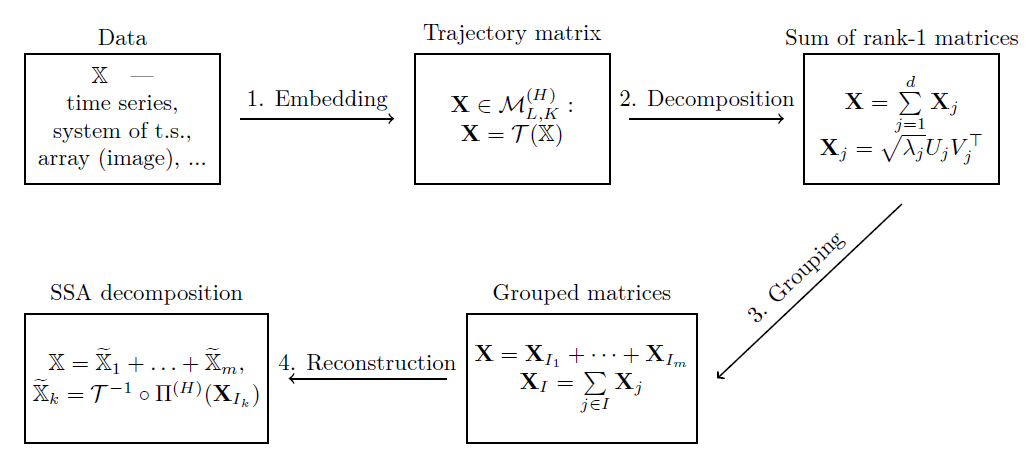
\includegraphics[width = 6in]{scheme_ssa}
	\end{center}
	\caption{Схема SSA-подобных алгоритмов.}
	\label{fig:ssa_scheme}
\end{figure}
\paragraph{Шаг 1. Вложение.} Первый шаг заключается в построении так называемой \textit{траекторной матрицы} $\mathbf{X} = \mathcal{T}\left(\mathbb{X} \right)$ с помощью оператора $\mathcal{T}$.
Обозначим $\mathcal{M}_{L,K}$ --- множество (вещественных или комплексных в случае CSSA) матриц размера $L \times K$, и за $\mathcal{M}_{L,K}^{(H)}$ --- множество (вещественных или комплексных в случае CSSA) ганкелевых матриц размера $L \times K$.
На данном шаге для каждого метода надо определить оператор $\mathcal{T}$ или траекторную матрицу $\mathbf{X}$.
Далее приведен  вид  оператора $\mathcal{T}$ или траекторной матрицы $\mathbf{X}$ для всех вариантов SSA-подобных методов.
\begin{enumerate}
\item 1D-SSA и одномерный вещественный ряд $\mathbb{X}= (x(1),\ldots,x(N))$ длины $N$.

Оператор $\mathcal{T}$ действует из пространства $\mathsf{R}^N$ в пространство $\mathcal{M}_{L,K}^{(H)}$ ганкелевых матриц размера $L \times K$:
\begin{equation*}
\mathcal{T}_{\text{1D-SSA}}(\mathbb{X}) = \begin{pmatrix}
			x(1) & x(2) & x(3) & \ldots & x({K}) \\
			x(2) & x(3) & x(4) & \ldots & x({K+1}) \\
			x(3) & x(4) & x(5) & \ldots & x({K+2}) \\
			\vdots &\vdots & \vdots & \ddots & \vdots \\
			x({L}) & x({L+1}) & x({L+2}) & \ldots & x({N})
			\end{pmatrix},
\end{equation*}

где $1<L<N$ называется \textit{длиной окна}, $K=N-L+1$.
\item CSSA и комплексный ряд $\mathbb{X}=\mathbb{X}^{(1)} + \I \,\mathbb{X}^{(2)}= \left(x^{(1)}(1) + \I\,x^{(2)}(1) ,\ldots,x^{(1)}(N) + \I\,x^{(2)}(N)\right)$.

Оператор $\mathcal{T}$ действует из пространства $\mathsf{C}^N$ в пространство $\mathcal{M}_{L,K}^{(H)}$ комплексных ганкелевых матриц размера $L \times K$, и траекторная матрица имеет такой же вид, как для 1D-SSA, только является комплексной.

\item MSSA и система $\mathbb{X}=\left(\mathbb{X}^{(1)},
 \ldots,\mathbb{X}^{(s)}\right)$ из $s$ временных рядов длины $N_p$, $\mathbb{X}^{(p)} = \left( x^{(p)}(j) \right)_{j=1}^{N_p}$, $p=1,\ldots,s$.

 В данном случае длиной окна $L$ будем называть $1< L < \min(N_p,p=1,\ldots,s)$. Определим также $K_p = N_p - L + 1$, $K = \sum_{p=1}^{s} K_p$. Траекторная матрица для многомерного ряда $\mathbb{X}$ --- это матрица размера $L \times K$ и вида
\begin{gather*}
\mathcal{T}_{\text{MSSA}} = \mathbf{X} = \left[ \mathbf{X}^{(1)}: \ldots :  \mathbf{X}^{(s)}  \right],
\end{gather*}
где $\mathbf{X}^{(p)}= \mathcal{T}_{\text{1D-SSA}} \left(\mathbb{X}^{(p)} \right)$ --- траекторная матрица одномерного ряда $\mathbb{X}^{(p)}$.
Другими словами, траекторная матрица многомерного ряда $\mathbb{X}$ представляет собой расположенные последовательно траекторные матрицы $\mathbf{X}^{(1)},\ldots, \mathbf{X}^{(s)}$ рядов $\mathbb{X}^{(1)}, \ldots, \mathbb{X}^{(s)}$.

\item 2D-SSA и поле $\mathbb{X}= \left(x(i,j) \right)_{i,j=1}^{N_x,N_y}$.

В этом случае длиной окна будем называть $(L_x, L_y)$, удовлетворяющие условиям $1 \leqslant L_x \leqslant N_x$, $1 \leqslant L_y \leqslant N_y$, $1 \leqslant L_x L_y \leqslant N_x N_y$. Положим $K_x = N_x - L_x + 1$ и $K_y = N_y - L_y + 1$. Также определим $L = L_x L_y$, $K = K_x K_y$.

Траекторная матрица для поля $\mathbb{X}$ --- это матрица размера $L \times K$ и вида
\begin{equation*}
\mathcal{T}_{\text{2D-SSA}}(\mathbb{X}) = \mathbf{X}= \begin{pmatrix}
			\mathbf{H}_1 & \mathbf{H}_2 & \mathbf{H}_3 & \ldots & \mathbf{H}_{K_y} \\
			\mathbf{H}_2 & \mathbf{H}_3 & \mathbf{H}_4 & \ldots & \mathbf{H}_{K_y+1} \\
			\mathbf{H}_3 & \mathbf{H}_4 & \mathbf{H}_5 & \ldots & \mathbf{H}_{K_y+2} \\
			\vdots &\vdots & \vdots & \ddots & \vdots \\
			\mathbf{H}_{L_y} & \mathbf{H}_{L_y+1} & \mathbf{H}_{L_y+2} & \ldots & \mathbf{H}_{N_y}
			\end{pmatrix}.
\end{equation*}
Матрица является блочно-ганкелевой с ганкелевыми блоками размера $L_x \times K_x$
\begin{equation*}
\mathbf{H}_j = \mathcal{T}_{\text{1D-SSA}}(\mathbb{X}_{:j})  = \begin{pmatrix}
			x(1,j) & x(2,j) & \ldots & x(K_x, j) \\
			x(2,j) & x(3,j) & \ldots & x(K_x+1, j) \\
			\vdots  & \vdots & \ddots & \vdots \\
			x(L_x, j) & x(L_x+1, j) & \ldots & x(N_x, j)
			\end{pmatrix},
\end{equation*}
где $\mathbb{X}_{:j}$ --- $j$-ый столбец матрицы $\mathbb{X}$.
\end{enumerate}

\paragraph{Шаг 2. Сингулярное разложение.}
На данном этапе происходит сингулярное разложение (SVD) матрицы $\mathbf{X}$ в сумму $d$ элементарных матриц
\begin{equation} \label{eq:svd}
    \mathbf{X}=\mathbf{X}_1+\ldots+\mathbf{X}_d,
\end{equation}
где
$\mathbf{X}_i=\sqrt{\lambda_i}U_i V_i^\mathrm{*}$, $d=\max\{i : \lambda_i > 0\}$,
$\lambda_1,\ldots,\lambda_d$ --- положительные собственные числа, взятые в неубывающем порядке $(\lambda_1\geqslant\ldots\geqslant\lambda_d\geqslant 0)$, и $U_1,\ldots,U_d$ --- соответствующие им ортонормированные собственные вектора матрицы  $\mathbf{X}\mathbf{X}^\mathrm{*}$, $V_i=\mathbf{X}^\mathrm{*} U_i/\sqrt{\lambda_i}$; символ $\mathrm{*}$ обозначает эрмитово сопряжение, что является операцией транспонирования для всех SSA-подобных методов кроме CSSA. 
Обычно в реальных примерах $d=L$.

Числа $\sqrt{\lambda_i}$ называются \emph{сингулярными числами}, $U_i$  и $V_i$ --- \emph{левыми} и \emph{правыми сингулярными векторами} матрицы  $\mathbf{X}$ соответственно.

\paragraph{Шаг 3. Группировка.}  Процедура группировки делит все множество индексов ${1,\ldots,d}$, полученных в результате разложения \eqref{eq:svd}, на $m$ не пересекающихся подмножеств $I_1,\ldots,\\ I_m$.
Результирующая матрица $\mathbf{X}_I$, соответствующая группе $I=\{i_1,\ldots,i_p\}$, определяется как $\mathbf{X}_I=\mathbf{X}_{i_1}+\ldots+\mathbf{X}_{i_p}$.
Вычислив такие матрицы для всех групп $I=I_1,\ldots,I_m$, получаем сгруппированный вид представления \eqref{eq:svd}:
\begin{equation}\label{eq:svd_group}
    \mathbf{X}=\mathbf{X}_{I_1}+\ldots+\mathbf{X}_{I_m}.
\end{equation}

\paragraph{Шаг 4. Восстановление.}
На последнем этапе каждая матрица разложения \eqref{eq:svd_group} переводится в форму исходного объекта $\mathbb{X}$. Преобразование выполняется оптимально в следующем смысле: для матрицы $\mathbf{Y} \in \mathcal{M}_{L,K}$ мы ищем объект $\widetilde{\mathbb{Y}}$, на котором достигается минимум $\|\mathbf{Y} -  \mathcal{T}(\widetilde{\mathbb{Y}})\|_{\mathcal{F}}$, где $\|\mathbf{Z}\|_{\mathcal{F}} = \sqrt{\sum_{i,j=1}^{L,K}(\mathbf{Z})_{ij}^2}$ --- норма Фробениуса.

Обозначим $\Pi^{(H)}: \mathcal{M}_{L,K} \rightarrow \mathcal{M}_{L,K}^{(H)}$ --- ортогональный проектор на $\mathcal{M}_{L,K}^{(H)}$ по норме Фробениуса. Тогда $\widetilde{\mathbb{Y}} = \mathcal{T}^{-1}\left( \Pi^{(H)} \mathbf{Y}\right)$.

Применяем преобразование к результирующим матрицам $\mathbf{X}_{I_k}$ и получаем восстановленные объекты $\widetilde{\mathbb{X}}_k =\mathcal{T}^{-1}\left( \Pi^{(H)} \mathbf{X}_{I_k}\right)$. Таким образом, исходный объект $\mathbb{X}$ раскладывается в сумму $m$ объектов исходного типа
\begin{equation*}
\mathbb{X} = \widetilde{\mathbb{X}}_1 + \ldots + \widetilde{\mathbb{X}}_m.
\end{equation*}
Если $m = d$ и $\mathbf{X}_{I_k} = \mathbf{X}_k$, то восстановленные объекты $\widetilde{\mathbb{X}}_k$ называются \textit{элементарными компонентами}.

\section{Свойства разложения для э-м гармоник}
В введении мы определили, что колебательная составляющаяся описывается суммой э-м гармоник. В данном разделе приведем определение и опишем свойства э-м гармоник для всех вариантов SSA-подобных алгоритмов.

\subsection{1D-SSA}
\label{sec:1d_ssa_theory}

Элементы вещественнозначного экспоненциально-модулированного гармонического ряда $\mathbb{S}$ имеют вид
\begin{equation} \label{eq:ex_mod_garm_1d}
 s(n) = a\, e^{\alpha n} \cos(2\pi\omega n + \phi),
\end{equation}
где $0 \leqslant \phi < 2\pi$, $a \not = 0$, $0<\omega \leqslant 0.5$, $\sin \phi \not = 0$ для $\omega = 0.5$.

Введем следующие обозначения: $L$ --- длина окна, параметр метода 1D-SSA, $K=N-L+1$, $\Lambda^{(1)}$ и $\Lambda^{(2)}$ --- подпространства строк и столбцов траекторной матрицы ряда $S_N$.

$L$-Ранг ряда $d$ --- это ранг его траекторной матрицы и, следовательно, количество левых или правых сингулярных векторов, соответствующих ненулевым сингулярным числам траекторной матрицы $\mathbf{X}$.

%Из вида ряда $\mathbb{S}$ и определения траекторной матрицы получается следующее простое утверждение.

\begin{Th} \cite[Section 5.1]{Golyandina.etal2001} \label{th:ex_mod_1d}
\begin{enumerate}
\item $L$-Ранг $d$ ряда $\mathbb{S}$, элементы которого имеют вид \eqref{eq:ex_mod_garm_1d},  равен $1$, если $\omega = 0.5$, в остальных случаях $d=2$.
\item Если $\omega \not = 0.5$, то подпространства $\Lambda^{(1)}$ и $\Lambda^{(2)}$ имеют базисы \\
\begin{gather*}
\{(1, e\cos(2\pi\omega),\ldots,e^{\alpha (L-1)}\cos(2\pi (L-1) \omega))^\mathrm{T}, \\
(0, e\sin(2\pi\omega),\ldots,e^{\alpha (L-1)}\sin(2\pi (L-1) \omega))^\mathrm{T}\} \quad \text{и} \\
\{(1, e\cos(2\pi\omega),\ldots,e^{\alpha (K-1)}\cos(2\pi (K-1) \omega))^\mathrm{T}, \\
(0, e\sin(2\pi\omega),\ldots,e^{\alpha (K-1)}\sin(2\pi (K-1) \omega))^\mathrm{T}\}.
\end{gather*}
соответственно.
\item В случае $\omega = 0.5$ одномерные $\Lambda^{(1)}$ и $\Lambda^{(2)}$ являются линейными оболочками векторов $(1,c,\ldots,c^{L-1})^{\mathrm{T}}$ и $(1,c,\ldots,c^{K-1})^{\mathrm{T}}$ соответственно, где $c = -e^{\alpha}$.
\end{enumerate}
\end{Th}

\begin{Th} \cite[Предложение 2.3]{Golyandina.etal2003} \label{th:1dssa_num}
Пусть $\alpha = 0$, $\omega \not = 0.5$ и $L\omega$  и $K\omega$ --- целые. Тогда собственные числа сингулярного разложения для ряда $\mathbb{S}$ с элементами вида \eqref{eq:ex_mod_garm_1d} одинаковы и имеют вид $\lambda_1=\lambda_2=a^2LK/4$.
\end{Th}

Из утверждения \ref{th:ex_mod_1d} следует, что для $\omega \not = 0.5$ ряд $\mathbb{S}$ имеет ровно два левых сингулярных вектора $U_1$ и $U_2$, соответствующих ненулевым собственным числам траекторной матрицы,
и что элементы векторов $U_1$ и $U_2$ можно представить в следующем виде:
\begin{gather} \label{eq:vectors_ex_mod_1d}
	u_k^{(1)} = a_1 e^{\alpha k} \cos(2\pi\omega k + \phi_1), \quad u_k^{(2)} = a_2 e^{\alpha k}\cos(2\pi\omega k + \phi_2),
\end{gather}
где $1 \leqslant k \leqslant L$, $0 \leqslant \phi_1, \phi_2 < 2\pi$, $a_1, a_2 \not = 0$.

\begin{Th}  \cite[Утверждение 8]{Zhornikova2016} \label{th:aboutU1U2_ex_mod_1d}
Пусть $\alpha = \alpha_N = C_1/N$, где $C_1$ --- некоторая константа, и $L=[\beta N]$, где $0<\beta<1$. Тогда для сингулярных векторов $U_1$ и $U_2$ ряда $\mathbb{S}$, элементы которых имеют вид \eqref{eq:vectors_ex_mod_1d}, выполняются соотношения: $\lim_{L \rightarrow \infty}{|\phi_1-\phi_2|}=\pi/2 \,\,(\mod \pi)$ и $\lim_{L \rightarrow \infty}{(a_1/a_2)} = 1$.
\end{Th}


Введем определение периодограммы ряда $\mathbb{Y}=(y(1),\ldots,y({M}))$ длины M:
\begin{gather}
\label{eq:per}
 \Pi_{\mathbb{Y}}^M(k/M) = \frac{M}{2}
\begin{cases}
2c_0^2 &\quad \text{для } k = 0, \\
c_k^2 + s_k^2 & \quad \text{для }  0 \leqslant k \leqslant M/2, \\
2c_{M/2}^2 & \quad \text{для } k = M/2   \text{, если } M \text{ четное},
\end{cases}
\end{gather}
где коэффициенты $c_k$ и $s_k$ получаются из разложения Фурье для ряда $\mathbb{Y}$:
\begin{gather*}
y(n) = c_0 + \sum_{k=1}^{\lfloor M/2 \rfloor}\left(c_k\cos(2\pi n k /M) + s_k\sin(2\pi n k/M) \right).
\end{gather*}

\begin{Th}  \cite[Утверждение 3.1]{Alexandrov2006} \label{th:aleks1}
Пусть $\alpha = 0$, $\omega \not = 0.5$ и $L\omega \in \mathsf{Z}$. Тогда для сингулярных векторов $U_1$, $U_2$ ряда $\mathbb{S}$, элементы которого имеют вид \eqref{eq:ex_mod_garm_1d}, выполняется
\begin{gather*}
\max_{0 \leqslant k \leqslant L} \Pi_{U_1}(k/L) = \max_{0 \leqslant k \leqslant L} \Pi_{U_2}(k/L) =  \Pi_{U_1}(\omega) =  \Pi_{U_2}(\omega) = 1.
\end{gather*}
\end{Th}

Пусть $P = (p_1,\ldots,p_L)^{\mathrm{T}}$ и $Q=(q_1,\ldots,q_L)^{\mathrm{T}}$ --- два вещественных вектора длины $L$. Введем для них меру 
\begin{gather} \label{eq:tau1} 
\tau(P, Q) := \hat{\D}(\Theta) =\frac{1}{L-1}\sum_{k=1}^{L-1}{\left(\theta_k  - \bar{\theta}\right)^2},
\end{gather}
где $\Theta=(\theta_1,\ldots,\theta_L)^{\mathrm{T}}$,
$\bar{\theta} = \sum_{k=1}^{L-1}{\theta_k}/(L-1)$, $\theta_k$ --- угол между  
$\left(p_k, q_{k}\right)^{\mathrm{T}}$ и $\left(p_{k+1}, q_{k+1}\right)^{\mathrm{T}}$, т.е.
\begin{gather*}
\theta_k = \arccos{\left(\frac{p_{k} p_{k+1} + q_{k} q_{k+1}}{\sqrt{p_{k}^2+q_{k}^2}\sqrt{p_{k+1}^2+q_{k+1}^2}}\right)}.
\end{gather*}

\begin{Th}  \cite[Теорема 1]{Zhornikova2016} \label{th:th_tau_1d}
Для сингулярных векторов $U_1$ и $U_2$  ряда $\mathbb{S}$, элементы которых имеют вид \eqref{eq:vectors_ex_mod_1d}, верны следующие утверждения.
\begin{enumerate}
\item \label{th:re_tau1}
Если $\alpha=0$ и $L\omega$ --- целое, то $\tau(U_1, U_2)=0$.
\item \label{th:re_tau2}
Если $\alpha = 0$ и  $L=[\beta N]$, где $0<\beta<1$, то $\lim_{L \rightarrow \infty}\tau(U_1, U_2) = 0$.
\item  \label{th:re_tau3}
Если $\alpha = \alpha_N = C_1/N$, где $C_1$ --- некоторая константа, и $L=[\beta N]$, где $0<\beta<1$, то $\lim_{L \rightarrow \infty}\tau(U_1, U_2) = 0$.
\end{enumerate}
\end{Th}

\subsection{CSSA}
\label{sec:cssa_theory}
Рассмотрим \textit{комплекснозначный экспоненциально-модулированный гармонический ряд} $\mathbb{S}$ с элементами:
\begin{equation} \label{eq:complex_exmodgarm}
 s(n) = e^{\alpha n} (a\cos(2\pi\omega n + \phi_1) + \I \,b\cos(2\pi\omega n + \phi_2)),
\end{equation}
где $0 \leqslant\phi_1, \phi_2 < 2\pi$, $a, b \not = 0$, $0<\omega \leqslant 0.5$, $\sin \phi_1 \not = 0$ или $\sin \phi_2 \not = 0$ для $\omega = 0.5$.

По-прежнему, $L$ --- длина окна, $K=N-L+1$, $\Lambda^{(1)}$ и $\Lambda^{(2)}$ --- подпространства строк и столбцов траекторной матрицы ряда $\mathbb{S}$, $d$ --- $L$-ранг ряда $\mathbb{S}$.

\begin{Th} \cite[Утверждение 3]{Zhornikova2016} \label{th:cssa_ex_mod_im_vec}
\begin{enumerate}
\item $L$-ранг $d$ ряда $\mathbb{S}$, элементы которого имеют вид \eqref{eq:complex_exmodgarm},  равен $1$, если $a=b$ и $|\phi_1 - \phi_2| = \pi/2 \,\,(\mod \pi)$ или $\omega = 0.5$, в остальных случаях $d=2$.
\item Если $\omega$ и $\phi_j$ такие, что $d = 2$, то пространства $\Lambda^{(1)}$ и $\Lambda^{(2)}$ имеют базисы
\begin{gather*}
\{(1, e\cos(2\pi\omega),\ldots,e^{\alpha (L-1)}\cos(2\pi (L-1) \omega))^{\mathrm{T}}, \\
(0, e\sin(2\pi\omega),\ldots,e^{\alpha (L-1)}\sin(2\pi (L-1) \omega))^{\mathrm{T}}\},  \quad \text{и} \\
\{(1, e\cos(2\pi\omega),\ldots,e^{\alpha (K-1)}\cos(2\pi (K-1) \omega))^{\mathrm{T}}, \\
(0, e\sin(2\pi\omega),\ldots,e^{\alpha (K-1)}\sin(2\pi (K-1) \omega))^{\mathrm{T}}\}
\end{gather*}
соответственно.
\item Если
 $a=b$ и $|\phi_1 - \phi_2| = \pi/2 \,\,(\mod \pi)$ одномерные пространства $\Lambda^{(1)}$ и $\Lambda^{(2)}$ натянуты на вектора $(1,c,\ldots,c^{L-1})^{\mathrm{T}}$ и $(1,c,\ldots,c^{K-1})^{\mathrm{T}}$ соответственно, где $c = e^{\I 2\pi\omega + \alpha}$. Если $\omega = 0.5$ одномерные $\Lambda^{(1)}$ и $\Lambda^{(2)}$ натянуты на вектора $(1,c,\ldots,c^{L-1})^{\mathrm{T}}$ и $(1,c,\ldots,c^{K-1})^{\mathrm{T}}$ соответственно, где $c = -e^{\alpha}$.
\end{enumerate}
\end{Th}

 Из утверждения \ref{th:cssa_ex_mod_im_vec} следует, что если $\omega$ и $\phi_j$ такие, что $d = 2$, то элементы сингулярных векторов $U_1$ и $U_2$ ряда $\mathbb{S}$ можно представить в следующем виде:
\begin{gather} \label{eq:uuu1}
	u_k^{(1)} = a_1 e^{\alpha k} \cos(2\pi\omega k + \phi_1) + \I \, b_1 e^{\alpha k} \cos(2\pi\omega k + \psi_1),\\ \label{eq:uuu2}
	u_k^{(2)} = a_2 e^{\alpha k}\cos(2\pi\omega k + \phi_2)+ \I \, b_2 e^{\alpha k} \cos(2\pi\omega k + \psi_2),
\end{gather}
где $1 \leqslant k \leqslant L$, $0 \leqslant \phi_j, \psi_j < 2\pi$, $a_j, b_j \not = 0$, $j=1,2$.

\begin{Th} \cite[Предложение 2.3]{Golyandina.etal2003} \label{th:cssa_num}
Пусть $\alpha = 0$, $\omega \not = 0.5$, $L\omega$ и $K\omega$ --- целые. Тогда
\begin{enumerate}
\item для комплексной гармоники $\mathbb{S}$, элементы которой имеют вид \eqref{eq:complex_exmodgarm}, в случае $d=2$ собственные числа имеют вид  $D^2LK$ и $E^2LK$, где
\begin{equation*}
D^2=(a^2+b^2-2ab\sin\phi)/4, \quad E^2=(a^2+b^2+2ab\sin\phi)/4
\end{equation*}
и $\phi=\phi_2-\phi_1$;
\item для комплексной гармоники $\mathbb{S}$, элементы которой имеют вид \eqref{eq:complex_exmodgarm}, в случае $d=1$ собственное число имеет вид $\lambda=a^2LK$.
\end{enumerate}
\end{Th}

Определение \eqref{eq:tau1} для меры $\tau$, используемое ниже в утверждении, дано в предыдущем разделе \ref{sec:1d_ssa_theory}.
\begin{Th}   \cite[Теорема 2]{Zhornikova2016} \label{th:th_tau_cssa}
Пусть $U_1$ и $U_2$ --- сингулярные вектора для ряда $\mathbb{S}$ с рангом $d=2$, записанные в виде \eqref{eq:uuu1} и \eqref{eq:uuu2} соответственно. Тогда верны следующие утверждения.
\begin{enumerate}
\item \label{th:complex_t_1}
Если $\alpha=0$ и $L\omega$ --- целое, то существует $0 \leqslant t < 1$, такое что
\begin{gather*}
\tau(\RE U_1, \RE e^{\I 2\pi t} U_2) + \tau (\IM U_1, \IM e^{\I 2\pi t} U_2) = 0.
\end{gather*}
\item \label{th:complex_t_4}
Если $\alpha = 0$ и $L=[\beta N]$, где $0<\beta<1$, то существует числовая последовательность $t = t_L$, принимающая значения в $[0,1)$, такая что
\begin{gather*}
\lim_{L \rightarrow \infty} (\tau (\RE U_1, \RE e^{\I 2\pi t} U_2) + \tau (\IM U_1, \IM e^{\I 2\pi t} U_2)) = 0.
\end{gather*}
\item \label{th:complex_t_5}
Если $\alpha = \alpha_N = C_1/N$, где $C_1$ --- некоторая константа, и $L=[\beta N]$, где $0<\beta<1$, то существует числовая последовательность $t = t_L$, принимающая значения в $[0,1)$, такая что
\begin{gather*}
\lim_{L \rightarrow \infty} (\tau (\RE U_1, \RE e^{\I 2\pi t} U_2) + \tau (\IM U_1, \IM e^{\I 2\pi t} U_2)) = 0.
\end{gather*}
\end{enumerate}
\end{Th}

Для случая $d=1$, т.е. когда в \eqref{eq:complex_exmodgarm} $a=b$ и $|\phi_1 - \phi_2| = \pi/2 \,\,(\mod \pi)$ обозначим единственный сингулярный вектор, соответствующий ненулевому сингулярному числу, как $U_1$.
По утверждению \ref{th:cssa_ex_mod_im_vec} элементы сингулярного вектора $U_1$ имеют вид
\begin{gather} \label{eq:vid_d1}
	u_k^{(1)} = c\,e^{2\pi \mathrm{i} \omega k + \alpha k},
\end{gather}
где $c$ --- некоторая константа.

\begin{Th}  \cite[Утверждение 14]{Zhornikova2016} \label{th:th_tau_cssa_d1}
Для сингулярного вектора $U_1$ ряда $S_N$ с рангом $d=1$, записанного в виде \eqref{eq:vid_d1},
 \begin{gather*}
 \tau(\RE U_1, \IM U_1)=0.
 \end{gather*}
\end{Th}


\subsection{MSSA}
\label{sec:mssa_theory}

Рассмотрим \textit{многомерный экспоненциально-модулированный гармонический ряд} $\mathbb{S} = \left(\mathbb{S}^{(1)},
 \ldots,\mathbb{S}^{(s)}\right)$, где элемент $p$-го ряда имеет вид
\begin{equation} \label{eq:em_mssa}
 s^{(p)}(n) = e^{\alpha n} a_p\cos(2\pi\omega n + \phi_p),
\end{equation}
где $0 \leqslant\phi_p < 2\pi$, $a_p \not = 0$, $0<\omega \leqslant 0.5$, $\sin \phi_p \not = 0$ для $\omega = 0.5$, $n=1,\ldots,N_p$, $p=1,\ldots,s$.

$L$ --- длина окна, $K_p = N_p - L + 1$, $K = \sum_{p=1}^{s} K_p$.

\begin{Th}  \cite[Предложение 2.2]{Golyandina.etal2003} \label{th:mssa_rank} \label{th:mssa_vec}
\begin{enumerate}
\item 
$L$-Ранг $d$ ряда $\mathbb{S}$, элементы которого задаются \eqref{eq:em_mssa}, равен $1$, если $\omega = 0.5$, в остальных случаях $d=2$.
\item Если $\omega \not = 0.5$, то подпространство $\Lambda^{(1)}$ имеет базис 
\begin{gather*}
\{(1, e\cos(2\pi\omega),\ldots,e^{\alpha (L-1)}\cos(2\pi (L-1) \omega))^\mathrm{T}, \\
(0, e\sin(2\pi\omega),\ldots,e^{\alpha (L-1)}\sin(2\pi (L-1) \omega))^\mathrm{T}\}. 
\end{gather*}
\item Если $\omega \not = 0.5$, то подпространство $\Lambda^{(2)}$ имеет базис 
\begin{gather*}
\{(c^{(1)}_1,\ldots,c_{K_1}^{(1)}; \ldots; c^{(s)}_1,\ldots,c_{K_s}^{(s)})^\mathrm{T},
(d^{(1)}_1,\ldots,d_{K_1}^{(1)}; \ldots; d^{(s)}_1,\ldots,d_{K_s}^{(s)})^\mathrm{T} \}, 
\end{gather*}
где 
\begin{gather*}
c^{(p)}_j = a_p \cos(2\pi j \omega + \phi_p) \quad \text{и}\quad d^{(p)}_j = a_p \sin(2\pi j \omega + \phi_p), \quad j=1,\ldots,K_p, \quad p=1,\ldots,s.
\end{gather*}
\item В случае $d=1$ одномерные $\Lambda^{(1)}$ и $\Lambda^{(2)}$ натянуты на вектора \\ $(1,c,\ldots,c^{L-1})^{\mathrm{T}}$ и $(1,c,\ldots,c^{K-1})^{\mathrm{T}}$ соответственно, где $c = -e^{\alpha}$.
\end{enumerate}
\end{Th}

\begin{Th} \cite[Предложение 2.3]{Golyandina.etal2003} \label{th:mssa_num}
Пусть $\alpha = 0$, $\omega \not = 0.5$ и $L\omega$  и $K\omega$ --- целые, $s=2$. Тогда собственные числа сингулярного разложения для двумерного ряда $\mathbb{S}$, элементы которого задаются \eqref{eq:em_mssa}, одинаковы и имеют вид $\lambda_1=\lambda_2=(a^2 + b^2)LK/4$.
\end{Th}

\subsection{2D-SSA}
\label{sec:2d_ssa_theory}
%В данном разделе приведем теоретические утверждения, относящиеся к 2D-SSA.

Согласно \cite{Golyandina.Usevich2010} определим элементы двумерной гармоники $\mathbb{S}$ с частотами $\omega^{(X)}$, $\omega^{(Y)}$:
\begin{gather} \label{eq:2d_cos_el}
\notag
s(k,l) =  \left(
\begin{matrix}
\cos(2\pi \omega^{(X)}k) \\ \notag
\sin(2\pi \omega^{(X)}k)
\end{matrix}
\right)^{\mathrm{T}}
 \left(
\begin{matrix}
a & b \\
c & d
\end{matrix}
\right)
 \left(
\begin{matrix}
\cos(2\pi \omega^{(Y)}l) \\ \notag
\sin(2\pi \omega^{(Y)}l)
\end{matrix}
\right),
\notag
\end{gather}
где $1 \leqslant k \leqslant N_x$, $1 \leqslant l \leqslant N_y$, хотя бы один коэффициент из  группы $\{a,b,c,d\}$ не равен нулю и
$\omega^{(X)}, \omega^{(Y)} \in (0,0.5)$.

Колебательная составляющая $\mathbb{H}$ --- это сумма  какого-то числа $c$ двумерных гармоник. Элементы $\mathbb{H}$ имеют вид
\begin{gather} \label{eq:2d_cos}
h(k,l) = \sum_{m=1}^{c}{s_m(k,l)},
\end{gather}
где $a_m(k,l)$ --- элементы гармоники $\mathbb{S}_m$, $m=1,\ldots,c$.
\begin{gather}
\notag
h(k,l) = \sum_{m=1}^{c}(a \cos(2\pi \omega^{(X)}k) \cos(2\pi \omega^{(Y)}l) +
b_m \cos(2\pi \omega^{(X)}k) \sin(2\pi \omega^{(Y)}l) + \\ \label{eq:2d_cos_el_2}
c_m \sin(2\pi \omega^{(X)}k) \cos(2\pi \omega^{(Y)}l) +
d_m \sin(2\pi \omega^{(X)}k) \sin(2\pi \omega^{(Y)}l)),
\end{gather}
где $1 \leqslant k \leqslant N_x$, $1 \leqslant l \leqslant N_y$, хотя бы один коэффициент из каждой группы $\{a_m,b_m,c_m,d_m\}$ не равен нулю, а также выполняются условия
\begin{align} \label{eq:2d_omega}
\begin{matrix}
(\omega_n^{(X)}, \omega_n^{(Y)}) \not = (\omega_m^{(X)}, \omega_m^{(Y)}), \quad \text{для } n \not= m,\\
\omega_m^{(X)}, \omega_m^{(Y)} \in (0,0.5).
\end{matrix}
\end{align}

Как и с предыдущих разделах, $(L_x, L_y)$-рангом будем называть ранг траекторной матрицы, обозначим его как $\rank_{L_x, L_y}$ . 

\begin{defn}
Будем говорить, что $\mathbb{X}$ --- \emph{поле конечного ранга}, если существуют такие $d$, $L_{x_0}$, $L_{y_0}$, что 
\begin{gather*}
1 \leqslant L_{x_0} < \lfloor N_x/2 \rfloor, \\
1 \leqslant L_{y_0} < \lfloor N_y/2 \rfloor, \\
1 \leqslant d <\leqslant L_{x_0} L_{y_0}, 
\end{gather*} 
и для любых $L_x$, $L_y$, для которых выполняется 
\begin{gather*}
L_{x_0} \leqslant \min(L_x,K_x), \,\, L_{y_0} \leqslant \min(L_y,K_y),
\end{gather*} 
имеет место равенство $\rank_{L_x, L_y}{\mathbb{X}} = d$.
\end{defn}

\begin{Th}[\cite{Golyandina.Usevich2010}, Proposition 4.7] \label{th:2d_rank_cos}
Для длины окна $(L_x, L_y)$ такой, что $L_x, L_y, K_x, \\K_y \geqslant 4c$ ряд $\mathbb{H}$, элементы которого определены в \eqref{eq:2d_cos_el}, является рядом конечного ранга и его ранг равен
\begin{gather*}
\rank_{L_x, L_y}(\mathbb{H}) = \sum_{m=1}^{c}{\nu_m}, \quad \text{где } \nu_m=2\rank
 \left(
  \begin{matrix}
a_m &b_m &c_m &d_m \\
d_m &-c_m &-b_m &a_m
\end{matrix}
\right).
\end{gather*}
\end{Th}

Про собственные числа двумерной гармоники $\mathbb{S}$ пока что нет известных результатов.

\section{Разделимость}
\label{sec:separability}
Очень важным понятием в теории SSA является разделимость, отвечающая на вопрос, при каких условия в результате SSA алгоритма, из суммы $\mathbb{X} = \mathbb{X}_1 + \mathbb{X}_2$ можно выделить каждое слагаемое по отдельности.

\subsection{Определение точной разделимости}
Пусть  $\mathbb{X}_1$,  $\mathbb{X}_2$ --- два объекта одного типа. Выберем некоторую длину окна $L$. Обозначим за $\mathbf{X}_1$  и  $\mathbf{X}_2$ траекторные матрицы объектов $\mathbb{X}_1$,  $\mathbb{X}_2$ соответственно.

Обозначим  $\Lambda^{(L,1)}$  и $\Lambda^{(L,2)}$  линейные пространства, порожденные столбцами траекторных матриц   $\mathbf{X}^{(1)}$  и  $\mathbf{X}^{(2)}$  соответственно. Аналогичные обозначения  $\Lambda^{(K,1)}$  и $\Lambda^{(K,2)}$  будем использовать для пространств, порожденных столбцами эрмитово сопряженных матриц $(\mathbf{X}^{(1)})^\mathrm{*}$  и  $(\mathbf{X}^{(2)})^\mathrm{*}$.

\begin{defn}
Объекты $\mathbb{X}_1$,  $\mathbb{X}_2$ называются \emph{слабо разделимыми}, если пространство $\Lambda^{(L,1)}$ ортогонально пространству $\Lambda^{(L,2)}$, и пространство $\Lambda^{(K,1)}$  ортогонально пространству $\Lambda^{(K,2)}$.
\end{defn}

\begin{defn}
Пусть объекты $\mathbb{X}_1$,  $\mathbb{X}_2$ слабо разделимы, и множество собственных чисел разложения
 траекторной матрицы одного ряда не пересекается с множеством собственных чисел сингулярного разложения второго ряда,
 тогда объекты $\mathbb{X}_1$,  $\mathbb{X}_2$ называются \emph{сильно разделимыми}.
\end{defn}

\subsection{Асимптотическая и приближенная разделимость}
Согласно разделу 6.1.2 \cite{Golyandina.etal2001} на основе меры ортогональности траекторных подпространств можно ввести понятия асимптотической разделимости по длине ряда, стремящейся к бесконечности, и, соответственно, приближенной разделимости.

Согласно тому же разделу 6.1.2 \cite{Golyandina.etal2001} в 1D-SSA э-м гармоника с частотой $\omega_1$ приближенно отделима от любой другой э-м гармоники c частотой $\omega_2 \not = \omega_1$, от экспоненты и от полиномиального или константного ряда.
Из \cite{Golyandina.etal2003} известно, что в  случаях CSSA и MSSA комплексная или многомерная э-м гармоника с частотой $\omega_1$ отделима от любой другой э-м гармоники c частотой $\omega_2 \not = \omega_1$ и от константного ряда. Для других вариантов рядов исследования еще не были проведены.  
Согласно \cite{Golyandina.Usevich2010} в случае 2D-SSA отдельмость более разнообразна, 
 э-м гармоника  приближенно отделима от любой другой э-м гармоники c другими частотами и константного поля, но, например, никакой другой ряд от константного поля отделить нельзя.  

Из вышесказанного следует, что для разных методов тренд должен приближенно отделяться от колебательной составляющей, а э-м гармоники с разными частотами должны приближенно отделяться друг от друга. Поэтому поставленная во введении задачи идентификации является осмысленной.

\subsection{Характеристика разделимости}
\label{sec:sep}
Чтобы проверить разделимость восстановленных компонент $\widetilde{\mathbb{X}}_1$ и $\widetilde{\mathbb{X}}_2$, мы должны проверить ортогональность траекторных матриц $\widetilde{\mathbf{X}}_{1}$ и $\widetilde{\mathbf{X}}_{2}$, им соответствующих. Удобной мерой их ортогональности является скалярное произведение Фробениуса $\langle \widetilde{\mathbf{X}}_{1}, \widetilde{\mathbf{X}}_{2}\rangle_\mathcal{F}$. Нормализованная мера ортогональности: $\rho(\widetilde{\mathbf{X}}_{1}, \widetilde{\mathbf{X}}_{2}) = \langle \widetilde{\mathbf{X}}_{1}, \widetilde{\mathbf{X}}_{2}\rangle_\mathcal{F}/ \left( \| \widetilde{\mathbf{X}}_{1} \|_{\mathcal{F}} \|\widetilde{\mathbf{X}}_{2}\|_{\mathcal{F}} \right)$.

Пусть $\mathbb{E}_k$ --- объект, $k$-ый элемент которого равен 1, а все остальные элементы равны 0. Тогда траекторная матрица $\mathbf{X}$ объекта $\mathbb{X}$ содержит $w(k) := \mathcal{T}(\mathbb{E}_k)$ раз $k$-ый элемент $x(k)$ объекта $\mathbb{X}$. Введем взвешенное скалярное произведение для двух объектов $\mathbb{Y}$ и $\mathbb{Z}$: $(\mathbb{Y}, \mathbb{Z})_w = \sum_k w(k) y(k) z(k)$. Скалярное произведение порождает норму $\|\mathbb{Y}\|_w=\sqrt{(\mathbb{Y}, \mathbb{Y})_w}$. Определим меру
\begin{gather*}
\rho(\widetilde{\mathbf{X}}_{1}, \widetilde{\mathbf{X}}_{2})_w = \frac{\left( \widetilde{\mathbf{X}}_{1}, \widetilde{\mathbf{X}}_{2}\right)_w }{\left( \| \widetilde{\mathbf{X}}_{1} \|_w \|\widetilde{\mathbf{X}}_{2}\|_w \right)},
\end{gather*}
которую будем называть \textit{w-корреляцией}.

Пусть $ \widetilde{\mathbf{X}}_{j}$ --- элементарная восстановленная компонента по элементарной группе $I_j = \{j\}$, тогда матрица с элементами $\rho_{ij}^{(w)} = \rho(\widetilde{\mathbf{X}}_{i}, \widetilde{\mathbf{X}}_{j})_w$ называется \textit{матрицей w-корреляций}.

\begin{Th} \cite[Corollary 6.2]{Golyandina.etal2001} \label{th:sep_wcor}
Если два вещественных одномерных ряда $\mathbb{X}_1$ и $\mathbb{X}_2$ слабо разделимы, то $(\mathbb{X}_1, \mathbb{X}_2)_w = 0$.
\end{Th}

\chapter{Обзор существующих методов автоматической идентификации для 1D-SSA}
\label{sec:1d_methods}
В данной главе рассматриваем одномерный вещественнозначный временной ряд длины $N$: $\mathbb{X}= (x(1),\ldots,x(N))$, $x(i) \in \mathsf{R}$. Проведем обзор существующих методов автоматической группировки, либо идентификации тренда, либо идентификации колебательной составляющей.

\section{Кластерный метод группировки} \label{sec:1D_wcor}
Данный метод описан в \cite{Golyandina.Zhigljavsky2012} и позволяет делать группировку элементарных компонент.
Будем называть данный метод \textit{кластерным методом группировки}.

Метод основан на свойствах матрицы $w$-корреляций $\{\rho^{(w)}_{ij}\}$ между $i$-ой и $j$-ой элементарными восстановленными компонентами, введенной в разделе \ref{sec:sep}.
Для одномерного вещественного ряда $\mathbb{X}$ коэффициенты $w(i)$ принимают вид
\begin{gather} \label{eq:w_i}
 w(i) =
\begin{cases}
i &\quad \text{для } 0 \leqslant i \leqslant L^*, \\
L^* & \quad \text{для } L^* \leqslant i \leqslant K^*, \\
N - i + 1 & \quad \text{для } K^* \leqslant i \leqslant N,
\end{cases}
\end{gather}
где $L^* = \min(L,K)$ и $K^* = \max(L,K)$.
Если взвешенная корреляция $\{\rho^{(w)}_{ij}\}$ имеет большое значение, значит, соответствующие компоненты имеют похожее поведение и должны быть включены в одну группу.

На вход метода поступает матрица $\{\rho^{(w)}_{ij}\}$. Далее к матрице $1 -\{|\rho^{(w)}_{ij}|\}$ применяется метод кластерного анализа, на выходе получается разбиение компонент на группы. Метод реализуется алгоритмом \ref{alg:wcor}.

 \begin{algorithm}[!hhh]
\caption{Кластерный метод автоматической идентификации}
\label{alg:wcor}
\begin{algorithmic}[1]
\REQUIRE На вход поступают данные и параметры.
\begin{enumerate}
\item \textbf{Данные}: матрица w-корреляций $\{\rho^{(w)}_{ij}\}$ между элементарными восстановленными компонентами.
\item \textbf{Параметры}: количество групп $m$, метод кластеризации.
\end{enumerate}
\ENSURE Группы индексов компонент.
\STATE  Применяем метод кластерного анализа к матрице $1 -\{|\rho^{(w)}_{ij}|\}$, как матрице расстояний, метод объединения (linkage) --- произвольный.
\STATE Получаем $m$ групп компонент из результатов кластерного анализа.
\end{algorithmic}
\end{algorithm}

Явным недостатком метода является тот факт, что матрица $w$-корреляций не всегда может явно разделяться на отдельные кластеры, и непонятно, насколько устойчивые результаты дает метод, так как в реальных данных мы имеем дело с приближенной разделимостью, и согласно утверждению \ref{th:sep_wcor} раздела \ref{sec:sep} равенство $\left(\mathbb{X}_1, \mathbb{X}_2 \right)_w = 0$ является лишь необходимым условием слабой разделимости.

\section{Кластерный метод группировки с использованием DFT}
Метод предложен и описан в \cite{Alvarez2013} и позволяет группировать компоненты с похожими частотными характеристиками. Будем называть данный метод \textit{кластерным  методом группировки с использованием DFT}.

Для начала авторы предлагают метод выбора длины окна $L$.
Ее выбирают следующим образом: увеличивают значение $\theta$, идя по множеству $\Theta = \{2,\ldots,N -2\}$ до тех пор, пока не выполнится:
\begin{gather}
\label{eq:theta_matrix}
\rank(\mathbf{X}^{\theta+1}) < \rank(\mathbf{X}^{\theta}),
\end{gather}
где $\mathbf{X}^{\theta}$ --- траекторная матрица, полученная с помощью $L = \theta$. Как только \eqref{eq:theta_matrix} выполнится, фиксируют $L = \theta$.

Заметим, что смысла в описанном выборе окна нет, так как для зашумленного ряда траекторная матрица является матрицей полного ранга.

Далее опишем сам метод, реализуемый алгоритмом \ref{alg:cluster_dft}.
Авторы статьи предполагают, что сингулярные числа шумовой компоненты всегда меньше сингулярных чисел сигнала (если уровень шума не очень большой, т.е. сигнал отделяется от шума, то это действительно так). Поэтому на первом шаге метода происходит отбор сингулярных чисел с помощью порога $\tau_\lambda$.

На втором шаге строим матрицу  $\mathbf{\hat U}$ из левых сингулярных векторов, соответствующих сингулярным числам, отобранным на первом шаге. К столбцам матрицы $\mathbf{\hat U}$ применяем дискретное преобразование Фурье (DFT), получаем матрицу $\mathbf{\hat F}$. Авторы отмечают, что вместо DFT можно использовать и другое преобразование, которое будет переводить сингулярный вектор в какую-то его характеристику.

На последнем шаге к столбцам матрицы данных $\mathbf{\hat F}$ применяем кластерный метод, где в качестве расстояния используется евклидова метрика. Авторы пишут, что можно использовать и другую метрику расстояния для кластерного анализа.

 \begin{algorithm}[!hhh]
\caption{Кластерный метод автоматической идентификации с использованием DFT}
\label{alg:cluster_dft}
\begin{algorithmic}[1]
\REQUIRE На вход поступают данные и параметры.
\begin{enumerate}
\item \textbf{Данные}: левые сингулярные вектора $\{U_i\}_{i=1}^{d}$, сингулярные числа $\{\sqrt{\lambda_i}\}_{i=1}^{d}$.
\item \textbf{Параметры}: порог $\tau_\lambda$.
\end{enumerate}
\ENSURE Группы индексов компонент.
\STATE  $\{ \lambda_1 \geqslant \lambda_2 \geqslant \ldots \geqslant \lambda_{d}\}$ --- квадраты сингулярных чисел, соответствующие траекторной матрице $\mathbf{X}$. Выбираем $m$ такое, что $\lambda_m$ --- первый квадрат сингулярного числа, для которого $\lambda_m / \sum_{k=1}^{d}\lambda_k < \tau_\lambda$.
\STATE $\mathbf{\hat U}$ --- матрица, составленная из левых сингулярных векторов, соответствующих числам $\{ \lambda_1 \geqslant \lambda_2 \geqslant \ldots \geqslant \lambda_m\}$. К столбцам матрицы $\mathbf{\hat U}$ применяем дискретное преобразование Фурье, получаем матрицу $\mathbf{\hat F}$.
\STATE К столбцам матрицы данных $\mathbf{\hat F}$ применяем кластерный метод, где в качестве расстояния используется евклидова метрика.
\STATE Получаем $m$ групп компонент из результатов кластерного анализа.
\end{algorithmic}
\end{algorithm}

Главный недостаток метода --- непонятно, как выбирать порог  $\tau_\lambda$, так как соотношение сигнала к шуму заранее неизвестно.  В своих примерах авторы использовали $\tau_\lambda = 0.025$.

\section{Метод низких частот для идентификации тренда}
\label{sec:1d_freq_method}
Данный метод описан в \cite{Golyandina.Zhigljavsky2012}, еще более подробно метод описан в \cite{Alexandrov2006}. Метод позволяет идентифицировать компоненты, относящиеся к тренду.
 Будем называть данный метод \textit{методом низких частот для тренда}.

Метод основан на том, что находит компоненты с похожими частотными характеристиками, как и предыдущий кластерный алгоритм \ref{alg:cluster_dft}. Вклад частоты определяется с помощью периодограммы, определенной для ряда $\mathbb{Y}=(y(1),\ldots,y({M}))$ длины M формулой \eqref{eq:per} в разделе \ref{sec:1d_ssa_theory}:
\begin{gather*}
 \Pi_{\mathbb{Y}}^M(k/M) = \frac{M}{2}
\begin{cases}
2c_0^2 &\quad \text{для } k = 0, \\
c_k^2 + s_k^2 & \quad \text{для }  0 \leqslant k \leqslant M/2, \\
2c_{M/2}^2 & \quad \text{для } k = M/2   \text{, если } M \text{ четное},
\end{cases}
\end{gather*}
где коэффициенты $c_k$ и $s_k$ получаются из разложения Фурье для ряда $\mathbb{Y}$:
\begin{gather*}
y(n) = c_0 + \sum_{k=1}^{\lfloor M/2 \rfloor}\left(c_k\cos(2\pi n k /M) + s_k\sin(2\pi n k/M) \right).
\end{gather*}
Определим для ряда $\mathbb{Y}$ и $0 \leqslant  \omega \leqslant 0.5$ меру
\begin{gather}
\label{eq:T_measure}
T(\mathbb{Y}; \omega) = \sum_{k: 0 \leqslant k/M \leqslant \omega} I_{\mathbb{Y}}^M(k/M),
\end{gather}
где $I_{\mathbb{Y}}^M(k/M) = \Pi_{\mathbb{Y}}^M(k/M) / \|\mathbb{Y}\|^2$, $\Pi_{\mathbb{Y}}^M(k/M)$ определено выше в \eqref{eq:per}. Так как $\|\mathbb{Y}\|^2  = \sum_{k=1}^{\lfloor M/2 \rfloor} \Pi_{\mathbb{Y}}^M(k/M)$, то мера $T(\mathbb{Y}; \omega)$ может рассматриваться как вклад частот, содержащихся в частотном интервале $[0, \omega)$.

Так как тренд --- это низкочастотная составляющая, то для его выделения логично рассматривать частотный интервал $[0, \omega)$, где $\omega$ является небольшим значением, $\omega$ нужно брать меньшим значений периодов гармоник, содержащихся в ряде, если они известны.
Для автоматической группировки также нужно выбрать порог $T_0$, и брать те компоненты, значение меры $T$ для которых больше $T_0$.

Получаем алгоритм \ref{alg:freq1d} для метода низких частот.
В реальных примерах часто подходят значения параметров $\omega = 0.01$ и $T_0$ --- от 0.8 до 0.9.

\begin{algorithm}[!hhh]
\caption{1D-SSA. Метод низких частот для тренда}
\label{alg:freq1d}
\begin{algorithmic}[1]
\REQUIRE На вход поступают данные и параметры.
\begin{enumerate}
\item \textbf{Данные}: группа индексов $I \in \{1,\ldots,d\}$; значение  $0 \leqslant  \omega \leqslant 0.5$; ряды $\mathbb{Y}_i$, $i \in I$: левые сингулярные вектора,
правые сингулярные вектора или элементарные восстановленные ряды.
\item \textbf{Параметры}: порог $0 \leqslant T_0 \leqslant 1$.
\end{enumerate}
\ENSURE Группа индексов компонент $J \subset I$, относящихся к тренду.
\STATE  Для каждого ряда $\mathbb{Y}_i$, $i \in I$, вычисляем значение $T(\mathbb{Y}_i; \omega)$ с помощью \eqref{eq:T_measure}.
\STATE $J$ --- группа индексов $i \in I$, таких что $T(\mathbb{Y}_i; \omega) \geqslant T_0$.
\end{algorithmic}
\end{algorithm}

\section{Частотный метод идентификации колебательной составляющей}
\label{sec:1d_pgram_method}

В введении мы определили, что колебательная составляющая описывается суммой э-м гармоник.
Рассмотрим алгоритм автоматической идентификации э-м гармоник, предложенный в \cite{Alexandrov2006}.
 Будем называть данный метод \textit{частотным методом идентификации колебательной составляющей}.

Метод основан на исследовании периодограмм сингулярных векторов, соответствующих ряду. Метод состоит из двух частей, на первом этапе проводится предварительная проверка, и сингулярные тройки, идентифицированные на этом этапе, проходят дополнительную проверку на втором этапе.

Как мы знаем из утверждения \ref{th:ex_mod_1d}, в случае 1D-SSA э-м гармоника \eqref{eq:ex_mod_garm_1d} может иметь ранг 1, если частота $\omega=0.5$, или ранг 2 в противном случае, т.е. э-м гармонике может соответствовать либо один сингулярный вектор, либо два.

Описанный далее метод автоматической идентификации компонент, соответствующих э-м гармоникам, проверяет
\begin{itemize}
\item для каждой пары сингулярных векторов тот факт, что последовательности их элементов описываются э-м гармониками с одинаковой частотой,
\item для каждого сингулярного вектора --- что последовательность его элементов описывается э-м гармоникой с периодом 2 ($\omega=0.5$).
\end{itemize}

\begin{remark}
Так как по утверждению \ref{th:1dssa_num} одномерному вещественному гармоническому ряду с $\omega \not = 0.5$ соответствует два равных собственных числа траекторной матрицы, и алгоритм SSA метода, описанный в разделе \ref{sec:ssa_alg}, сортирует компоненты сингулярного разложения по значению собственных чисел, то
для идентификации гармоник ранга 2 достаточно рассматривать только последовательные пары сингулярных векторов.
\end{remark}

Согласно разделу \ref{sec:1d_ssa_theory}, гармоническому ряду вида \eqref{eq:ex_mod_garm_1d} соответствует два сингулярных вектора вида \eqref{eq:vectors_ex_mod_1d} с одинаковыми частотами.

Первый этап метода основан на том факте, что если для гармоники ($\alpha = 0$) с частотой $\omega$ и длины окна $L$ выполняется: $L \omega \in \mathsf{Z}$, то периодограммы ее сингулярных векторов равны $\Pi_{U_j}^L(k/L)=\chi_{\omega}(k/L)$ (где $\chi_{\omega}(\cdot)$ --- индикатор множества $\{\omega\}$).
C учетом наличия только приближенной разделимости, $L\omega \not \in \mathsf{Z}$ и $\alpha \not = 0$,
на первом этапе метода из всех последовательных пар сингулярных векторов выбираются такие, для которых аргументы максимумов периодограмм больше 0 и близки, т.е. отличаются друг от друга не более чем на $s_0/L$ (где $s_0 \in \mathsf{Z}_+$ --- фиксированный параметр метода):
\begin{gather} \label{eq:I_1_P}
I_1^{(\mathbb{P})} = \{ (i, i+1): \quad \theta_1 \theta_2 >0, \quad L |\theta_i - \theta_{i+1}| \leqslant s_0, \quad 1 \leqslant i \leqslant d -1  \},
\end{gather}
где $\theta_j = \argmax_{0 < k \leqslant L/2} \{\Pi_{U_j}^L(k/L)\}$ --- аргумент максимума периодограммы $\Pi_{U_j}^{L}$ сингулярного вектора $U_j$.

Аналогично каждый сингулярный вектор проверяется на соответствие гармонике с частотой 0.5:
\begin{gather} \label{eq:I_2_P}
I_2^{(\mathbb{P})} = \{i: \quad  L |\theta_{i} - 0.5 | \leqslant s_0, \quad 1 \leqslant i \leqslant d\}.
\end{gather}

Результатом первого этапа являются множества индексов $I_1^{(\mathbb{P})}$ и $I_2^{(\mathbb{P})}$ сингулярных векторов. $I_1^{(\mathbb{P})}$ --- пары номеров сингулярных векторов, идентифицированных как соответствующие э-м гармоникам с $0 < \omega < 0.5$.  $I_2^{(\mathbb{P})}$ --- номера сингулярных векторов, идентифицированных как соответствующие э-м гармонике с $\omega = 0.5$.

\begin{defn} \label{def:rho}
Пусть ${\cal{A}}= \{W_j\}$, $W_j$ --- конечное множество вещественных векторов  векторов, обозначим мощность множества как $\# {\cal{A}}$. Введем функцию $\rho_{\cal{A}}$, определенную на множестве ${\cal{A}}$:
\begin{gather*}
\rho_{{\cal{A}}}(k/L) = \frac{1}{\#{\cal{A}}} \sum_{W_j \in {\cal{A}}}{\Pi^{L}_{W_j}{(k/L)}}.
\end{gather*}
\end{defn}

Ввиду утверждения \ref{th:aleks1} раздела \ref{sec:1d_ssa_theory}, для того чтобы проверить, что сингулярные вектора с номерами $j, j + 1$ соответствуют гармонике, необходимо убедиться, что максимумы их периодограмм достигаются в одной точке, и что каждый из них при этом имеет значение, близкое к 1, так как э-м гармонике с частотой $\omega$: $L \omega \not \in \mathsf{Z}$ тоже соответствует большое значение максимума периодограммы (хоть и меньшее 1), потому что ее периодограмма имеет один четко выраженный пик.  Именно это и проверяется на втором этапе метода.

До работы \cite{Alexandrov2006}, на основе которой мы описываем метод, данный принцип проверки был предложен в работе \cite{Vautard1992}, однако сама идея не нова и была предложена еще в 1929~г. Фишером в статье \cite{Fisher1929}.

Таким образом, на втором этапе метода
 требуется выбрать порог $\rho_0$ для рассматриваемой меры
\begin{gather} \label{eq:rho_ij}
\rho_{i,j} := \max_{0 < k \leqslant L/2}{\left(\rho_{\{U_i,U_j\}}(k/L) + \rho_{\{U_i,U_j\}}((k+1)/L)\right)},
\end{gather}
где $U_i$, $U_j$ --- пара сингулярных векторов с индексами из множества индексов $I_1^{(\mathbb{P})}$, отобранных на первом этапе.

Для идентификации компонент, относящихся к гармонике с частотой 0.5, мера имеет вид
\begin{gather}\label{eq:rho_i}
\rho_{i} := \rho_{\{U_i\}}((\lfloor L/2 \rfloor)/L) + \rho_{\{U_i\}}((\lfloor L/2 \rfloor + 1)/L),
\end{gather}
где $i \in I_2^{(\mathbb{P})}$.

Итоговым результатом  частотного метода, реализуемого алгоритмом \ref{alg:1d_pgram}, являются индексы 
\begin{gather} \label{eq:pgram_I_p}
I^{(\mathbb{P})} = \{ (i,j) \in I_1^{(\mathbb{P})}: \rho_{i,j} \geqslant\rho_0 \} \cup \{ i \in I_2^{(\mathbb{P})}: \rho_{i} \geqslant\rho_0 \}.
\end{gather}

\begin{algorithm}[!hhh]
\caption{1D-SSA. Частотный метод для колебательной составляющей}
\label{alg:1d_pgram}
\begin{algorithmic}[1]
\REQUIRE  На вход поступают данные и параметры.
\begin{enumerate}
\item \textbf{Данные}: левые сингулярные вектора $\{U_i\}_{i=1}^{d}$.
\item \textbf{Параметры}: параметр $s_0 \in \mathsf{Z}_{+}$, порог $\rho_0 \in [0,1]$.
\end{enumerate}
\ENSURE Группа индексов компонент $I^{(\mathbb{P})}$, относящихся к колебательной составляющей.
\STATE По $\{U_i\}_{i=1}^{d}$ получаем группу индексов $I_1^{(\mathbb{P})}$ с помощью $s_0$ и \eqref{eq:I_1_P} и группу индексов $I_2^{(\mathbb{P})}$ с помощью $s_0$ и \eqref{eq:I_2_P}.
\STATE Получаем группу индексов $I^{(\mathbb{P})}$ по $\{U_j\}_{j \in I_1^{(\mathbb{P})} \cup I_2^{(\mathbb{P})}}$ и $\rho_0$ с помощью \eqref{eq:pgram_I_p}.
\end{algorithmic}
\end{algorithm}

Автор \cite{Alexandrov2006} советует брать $s_0 = 1$, а для выбора порога $\rho_0$ не дано четких рекомендаций, что является основным недостатком метода. Еще одним недостатком метода является тот факт, что его можно строго обосновать только для немодулированных гармоник ($\alpha = 0$).

\section{Метод группировки Н. В. Абалова, В. В. Губарева}
Метод предложен в статье \cite{Abalov2015} и позволяет делать группировку элементарных компонент. Метод рассматривает пары компонент и относит их к какой-то группе, поэтому в первую очередь метод применим для колебательной составляющей.    Будем называть данный метод \textit{методом группировки Н. В. Абалова, В. В. Губарева}.

Метод комбинирует две идеи. На первом шаге учитывается близость собственных чисел, т.е. вкладов компонент. На втором шаге учитывается похожесть компонент в смысле большой корреляции между ними или близости частот.
Для вещественной гармоники метод легко обосновывается с помощью утверждения \ref{th:1dssa_num} про равные собственные числа и вида сингулярных векторов \eqref{eq:vectors_ex_mod_1d}, имеющих одинаковые частоты.
Опишем общую схему метода.
\begin{enumerate}
\item Для всех элементарных компонент рассчитываем матрицу близости собственных чисел (квадратов сингулярных чисел) $\Delta = \{\delta_{ij}\}$, $i,j=1,\ldots,d$, где
\begin{gather}
\label{eq:delta}
\delta_{ij} = \frac{\min_{i, j}(\lambda_i, \lambda_j)}{\max_{i,j}(\lambda_i, \lambda_j)}.
\end{gather}
\item Рассчитываем матрицу <<смежности>> компонент $\mathbf{G}=\{g_{ij}\}$, $i,j = 1,\ldots,d$,
\begin{gather} \label{eq:g_ij}
g_{ij} =
\begin{cases}
c_{ij}, &\quad \delta_{ij} \geqslant \rho_1, \\
0, &\quad \text{иначе},
\end{cases}
\end{gather}
где $c_{ij}$ --- бинарный показатель близости двух компонент (далее будет рассмотрено два таких показателя  $c^{'}_{ij}$ и  $c^{''}_{ij}$).

Итогом выполнения операций 1--2 является матрица группировки $\mathbf{G}$, содержащая 1 в ячейках $i,j$, если пара компонент $i,j$ принадлежит одной группе, иначе 0.
\item Объединяем в одну группу составляющей ряда те  компоненты, для которых $g_{ij}~=~1$.
\end{enumerate}

Первый показатель близости $c_{ij} = c^{'}_{ij}$ основан на использовании
степени коэффициента связи между значениями периодограмм восстановленных компонент $\mathbb{X}_i$, $\mathbb{X}_j$ (например, коэффициента корреляции Пирсона, Спирмена, корреляционных отношений и т.п.). Чем выше значение $\rho_1$, тем жестче отбор.
Здесь $c^{'}_{ij} = 1$ тогда и только тогда, когда $\corr(\mathbb{X}_i, \mathbb{X}_j) \geqslant \rho_c$, $\rho_c \in [0,1]$.

Второй показатель близости $c_{ij} =c^{''}_{ij}$ сравнивает множества частот двух компонент, соответствующих максимальным значениям периодограммы.
Обозначим
$K_{\mathbb{X}_j} = \max_{0\leqslant k \leqslant L/2}\left(\Pi_{\mathbb{X}_j}(k)\right)$ --- максимальное значение периодограммы восстановленной компоненты $\mathbb{X}_j$;
\begin{gather} \label{eq:f_j}
F_{\mathbb{X}_j} =  \{ k: \Pi_{\mathbb{X}_j}(k) \geqslant \rho_p K_{\mathbb{X}_j}  \}, j = 1,\ldots, d.
\end{gather}
Множество $F_{\mathbb{X}_j}$ упорядочено по возрастанию, $\rho_p$ --- задаваемая величина порога, которая позволяет регулировать исключение низких значений периодограмм.

В данном случае $c^{''}_{ij}=1$ тогда и только тогда, когда для любого $h=1,\ldots,m$ имеем $|F_{\mathbb{X}_i}(h) - F_{\mathbb{X}_j}(h)|/ L/2 < \rho_2$, где $F_{\mathbb{X}_i}(h)$ --- $h$-ое значение индекса частоты из множества $F_{\mathbb{X}_i}$, $\rho_2$ --- порог предельного расхождения индекса частот,  $\rho_2 \in [0,1]$, $m = \min\left(\#F_{\mathbb{X}_i}(h), \#F_{\mathbb{X}_j}(h) \right)$. Чем меньше значение $\rho_2$, тем жестче условие.

Авторы статьи говорят, что использование показателя $c^{''}_{ij}$ должно позволить
учесть размытие и слабое смещение пиковых значений периодограмм при повышении уровня шума.
Для примеров авторы статьи брали $\rho_1 =\rho_c =\rho_p = 0.8$, $\rho_2 = 0.05$.

Алгоритм \ref{alg:1d_abalov} реализует описанный метод.

\begin{algorithm}[!hhh]
\caption{1D-SSA. Метод группировки Н. В. Абалова, В. В. Губарева}
\label{alg:1d_abalov}
\begin{algorithmic}[1]
\REQUIRE На вход поступают данные и параметры.
\begin{enumerate}
\item \textbf{Данные}: элементарные восстановленные ряды $\{\mathbb{X}_i\}_{i=1}^{d}$, сингулярные числа $\{\sqrt{\lambda_i}\}_{i=1}^{d}$.
\item \textbf{Параметры}: пороги $\rho_1, \rho_2, \rho_c, \rho_p  \in [0,1]$.
\end{enumerate}
\ENSURE Группы индексов компонент.
\STATE  С помощью квадратов сингулярных чисел $\{\sqrt{\lambda_i}\}_{i=1}^{d}$ вычисляем матрицу $\Delta = \{\delta_{ij}\}$ с помощью \eqref{eq:delta}.
\STATE Вычисляем матрицу $\mathbf{G}=\{g_{ij}\}$ с помощью $\{\mathbb{X}_i\}_{i=1}^{d}$ с помощью \eqref{eq:g_ij}, где\\
либо $c_{ij} = c_{ij}^{'}$, $c_{ij}^{'} = 1$, если  $\corr(\mathbb{X}_i, \mathbb{X}_j) \geqslant \rho_c$;

либо $c_{ij} = c_{ij}^{''}$, с помощью \eqref{eq:f_j} для каждого $j = 1,\ldots, d$ вычисляем множество $F_{\mathbb{X}_j}$, $c_{ij}^{''} = 1$, если $|F_{\mathbb{X}_i}(h) - F_{\mathbb{X}_j}(h)|/ L/2 < \rho_2$ для любого $h=1,\ldots,m$, $m = \min\left(\#F_{\mathbb{X}_i}(h), \#F_{\mathbb{X}_j}(h) \right)$.
\STATE К одной группе относим те индексы $i,j$, для которых $g_{ij} = 1$.
\end{algorithmic}
\end{algorithm}


Отметим, что если в случае $c_{ij}^{'}$ брать не просто корреляции, а взвешенные корреляции, определение которых дано в разделе \ref{sec:sep}, то получится кластерный метод группировки из раздела \ref{sec:1D_wcor} с некоторыми ограничениями на значения матрицы из-за пункта 1 рассматриваемого алгоритма \ref{alg:1d_abalov}. Если же брать просто корреляции, непонятно почему метод будет работать.

\section{Обзор приложений методов}

\subsection{Phil. J. Watson <<Identifying the Best Performing Time Series
Analytics for Sea Level Research>> \cite{Watson2016} \cite{Watson2016b}}

SSA применяется к данным  про уровень морей. Автор выделяет сигнал (средний уровень моря), предполагая, что он нелинейный и нестационарный. Применяется метод низких частот автоматической идентификации, реализуемый алгоритмом \ref{alg:freq1d} из раздела \ref{sec:1d_freq_method}, с частотой $\omega=0.01$ и порогом $T_0 = 0.75$.

\subsection{F. Romeroa, F.J. Alonsoa, J. Cuberob, G. Galán-Marína <<An automatic SSA-based de-noising and smoothing technique for surface electromyography signals>>
 \cite{Romeroa2015}}

SSA применяется к данным электромиографии (surface electromyography).
Весь алгоритм анализа довольно длинный, автоматическая идентификация применяется только на одном этапе.
Используется кластерный метод автоматической идентификации, реализуемый алгоритмом \ref{alg:wcor} из раздела \ref{sec:1D_wcor}. К матрице w-корреляций применяется k-means, выбирается группа, для которой среднеквадратичная ошибка с исходным сигналом наименьшая.

\subsection{Michael Leonard and Bruce Elsheimer <<Automatic Singular Spectrum Analysis and Forecasting>>
 \cite{Leonard2017}}

Статья посвящена функциям в языке программирования SAS, позволяющим делать SSA и автоматическую группировку. Снова применяется кластерный метод идентификации  с использованием матриц w-корреляций, реализуемый алгоритмом \ref{alg:wcor}. Группы выбираются таким образом, чтобы в любой группе $I_m$ значение $\rho^{(w)} _{ij}$ было близко к 1 для любых $i, j \in I_m$. Уровень близости к 1 можно задавать с помощью порога: если все корреляции больше этого порога, то значения относятся в одну группу. В пакете по умолчанию выбрано значение для порога $0.9$.

\chapter{Метод идентификации колебательной составляющей по регулярности углов для 1D-SSA}
\label{sec:tau1}
\section{Описание и обоснование метода}
Идея данного метода идентификации колебательной составляющей была предложена в моей бакалаврской работе \cite{Zhornikova2016} и основывается на свойствах специальной меры, которая была введена в разделе \ref{sec:1d_ssa_theory}.
Приведем определение меры снова.
Для вещественных векторов $P = (p_1,\ldots,p_L)^{\mathrm{T}}$ и $Q=(q_1,\ldots,q_L)^{\mathrm{T}}$ длины $L$: 
\begin{gather*} 
\tau(P, Q) := \hat{\D}(\Theta) =\frac{1}{L-1}\sum_{k=1}^{L-1}{\left(\theta_k  - \bar{\theta}\right)^2},
\end{gather*}
где $\Theta=(\theta_1,\ldots,\theta_L)^{\mathrm{T}}$,
$\bar{\theta} = \sum_{k=1}^{L-1}{\theta_k}/(L-1)$, $\theta_k$ --- угол между  
$\left(p_k, q_{k}\right)^{\mathrm{T}}$ и $\left(p_{k+1}, q_{k+1}\right)^{\mathrm{T}}$, т.е.
\begin{gather*}
\theta_k = \arccos{\left(\frac{p_{k} p_{k+1} + q_{k} q_{k+1}}{\sqrt{p_{k}^2+q_{k}^2}\sqrt{p_{k+1}^2+q_{k+1}^2}}\right)}.
\end{gather*}
Отметим, что так как $\theta_k$ --- это результат применения функции $\arccos$, то значения $\theta_k$ меняются от $0$ до $\pi$. 

По замечанию 3 из  \cite{Zhornikova2016}:
равенство $\tau(P, Q) =0$ означает, что все углы между последовательными точками $(p_k, q_k)^{\mathrm{T}}$ двумерной диаграммы векторов $P$ и $Q$ одинаковые. Если при этом нормы этих векторов монотонно меняются по $k$, то на двумерных диаграммах получатся <<спирали>>.

Для $d=2$ в условиях утверждения \ref{th:th_tau_1d} из раздела \ref{sec:1d_ssa_theory} при достаточно больших $L$ по описанному замечанию ряд \eqref{eq:ex_mod_garm_1d} можно идентифицировать с помощью двумерной диаграммы сингулярных векторов $U_1$ и $U_2$ --- она будет обладать свойствами, близкими к свойствам, соответствующих нулевому значению меры $\tau$. На рис. \ref{fig:re_ex_mod_diagram} приведены примеры получающихся изображений со <<спиралями>> для рядов с $N=99$, $L=50$. 

\begin{figure}[h] 
    \centering
   \begin{subfigure}[b]{0.3\textwidth}
       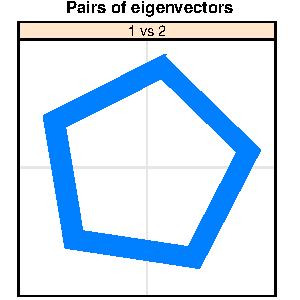
\includegraphics[width=\textwidth]{re_ex_mod_omega_1_5}
        \caption{$\omega=1/5$, $\alpha = 0.005$, \\$C_1 = 0.495$, $\tau =1.3e-05$.}

    \end{subfigure}
    \begin{subfigure}[b]{0.3\textwidth}
        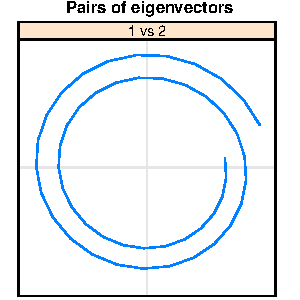
\includegraphics[width=\textwidth]{re_ex_mod_omega_1_25}
        \caption{ $\omega=1/25$, $\alpha = 0.009$, $C_1 = 0.891$, $\tau =$4.2e-05.}
    \end{subfigure}
    \begin{subfigure}[b]{0.3\textwidth}
        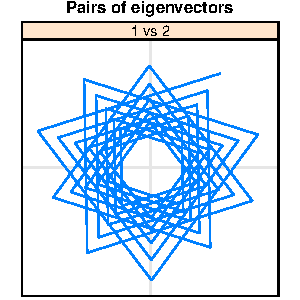
\includegraphics[width=\textwidth]{re_ex_mod_omega_3_10}
       \caption{$\omega=3/10$, $\alpha = 0.02$,\\ $C_1 = 1.98$, $\tau =$0.2e-03.}
    \end{subfigure}
    \caption{Двумерные диаграммы сингулярных векторов вещественных э.-м. гармоник, $N=99$, $L=50$, $\beta=1/2$.}
    \label{fig:re_ex_mod_diagram}
\end{figure} 

Отметим, что на практике мы не имеем дела с рядами бесконечной длины, поэтому для ряда конечной длины $N$ с константным значением $\alpha$ условие $\alpha = C_1/N$ означает не слишком большое значение $e^{\alpha N}$, т.е. ограниченность диапазона изменений значений ряда.


Если число э-м гармоник, которые хотим идентифицировать, известно, то алгоритм состоит просто в отборе пар векторов $U_i$ и $U_{i+1}$ с минимальными значениями меры  $\tau(U_i, U_{i+1})$, $i=1,\ldots, d-1$.

В случае, когда число
э-м гармоник неизвестно, в работе \cite{Zhornikova2016} было предложено отбирать пары сингулярных векторов с
помощью порога, т.е. к э-м гармонике относить те вектора $U_i$ и $U_{i+1}$, значение  $\tau(U_i, U_{i+1})$ для которых меньше заданного порога, но в работе не было дано никаких обоснований для выбора порога. 
Поэтому в данной главе приведем эмпирические обоснования для выбора порога и проведем численные исследования на примере зашумленного э-м косинуса.    

Отметим, что метод не работает для случая $\omega = 0.5$. Поэтому в данной главе мы его не рассматриваем.

Будем называть данный метод \textit{методом идентификации колебательной составляющей по регулярности углов}.


\section{Алгоритм метода}
Все объяснения, приводимые в предыдущем разделе, объясняли, почему для сингулярных векторов э-м гармоники значение меры $\tau$ будет равно 0. Встает вопрос, может ли получится значение $\tau$, близкое к 0, для сингулярных векторов не э-м гармоники. 

Например, если для каких-то векторов $P$ и $Q$ получаются хоть и разные, но маленькие значения углов $\theta_k$, заданных в определении \eqref{eq:tau1} меры $\tau$, то и значение дисперсии $\hat{\D}(\Theta)$ из этого же определения будет маленьким. 
Для борьбы с данной проблемой будем использовать в алгоритмах нормированный вариант меры $\tau$ от векторов $P = (p_1,\ldots,p_L)^{\mathrm{T}}$ и $Q=(q_1,\ldots,q_L)^{\mathrm{T}}$:
\begin{gather} \label{eq:tau_norm}
\tilde{\tau}(P, Q) := \frac{\tau(P, Q)}{\min(1, \bar{\theta}^2)} =\frac{\hat{\D}(\Theta)}{\min(1, \bar{\theta}^2)} =\frac{1}{(L-1) \min(1, \bar{\theta}^2)}\sum_{k=1}^{L-1}{\left(\theta_k  - \bar{\theta}\right)^2},
\end{gather} 
где, как и ранее, $\Theta=(\theta_1,\ldots,\theta_L)^{\mathrm{T}}$,
$\bar{\theta} = \sum_{k=1}^{L-1}{\theta_k}/(L-1)$, $\theta_k$ --- угол между  
$\left(p_k, q_{k}\right)^{\mathrm{T}}$ и $\left(p_{k+1}, q_{k+1}\right)^{\mathrm{T}}$.

Деление на $\min(1, \bar{\theta}^2)$ может только увеличить значение меры, поэтому оно борется с проблемой малых значений углов. Малые значения могут иметь углы и для сингулярных векторов э-м гармоники, но для них дисперсия будет близка к нулю и нормировка не сыграет существенной роли.

Для $\tilde{\tau}$ так же, как и для $\tau$, выполняется утверждение \ref{th:th_tau_1d}, так как если $\tau(P, Q) = 0$, то, очевидно, и $\tilde{\tau}(P, Q) = 0$. 

Как уже говорилось в предыдущем разделе, метод имеет две модификации: для случая, когда число э-м гармоник известно, и для случая с неизвестным числом э-м гармоник. Эти две модификации различаются критериями остановок в конце алгоритма \ref{alg:1dtau_2}, представленного ниже.

\begin{algorithm}[!hhh]
\caption{1D-SSA. Метод идентификации по регулярности углов для колебательной составляющей}
\label{alg:1dtau_2}
\begin{algorithmic}[1]
\REQUIRE На вход поступают данные и параметры.
\begin{enumerate}
\item \textbf{Данные}: число компонент $r$; левые сингулярные вектора $\{U_j\}_{j=1}^{r}$.\\
\item \textbf{Параметры}: количество э-м гармоник $m \leqslant r/2$, либо порог $t_0 \geqslant 0$, в зависимости от критерия остановки.
\end{enumerate}
\ENSURE Группа индексов сингулярных векторов $J$, относящихся к колебательной составляющей.
\STATE По $\{U_i\}_{i=1}^{r}$ вычисляем и упорядочиваем по возрастанию значения $\tilde{\tau}(U_j, U_{j+1})$, $j=1,\ldots, r-1$ с помощью \eqref{eq:tau_norm}. 
При вычислении для каждого $j = 2,\ldots,r-1$ проверяем: если $\tilde{\tau}(U_j, U_{j+1}) < \tilde{\tau}(U_{j-1}, U_{j})$, то выкидываем из рассмотрения значение $\tilde{\tau}(U_{j-1}, U_{j})$; иначе выкидываем $\tilde{\tau}(U_j, U_{j+1})$.
 Полученные значения: $\tau_1, \ldots, \tau_{\lfloor r/2 \rfloor}$.
\STATE Два варианта критерия остановки. Идем по множеству $i=1,\ldots,\lfloor r/2 \rfloor$
\begin{enumerate}
\item либо пока $i < m$;
\item либо пока $\tau_i < t_0$.
\end{enumerate}
$i_0$ --- момент остановки.
\STATE $J$ --- индексы $j$, $j+1$ сингулярных векторов $U_j$ и $U_{j+1}$, участвующих в вычислении  значений $\tau_1, \ldots, \tau_{i_0 - 1}$.
\end{algorithmic}
\end{algorithm}

\begin{remark}
На вход алгоритма могут подаваться не только первые $r$ сингулярных векторов. Может подавать любое множество последовательных векторов (множество, где индекс каждого следующего вектора на один больше предыдущего) из множества $\{U_j\}_{j=1}^{d}$. В алгоритме для простоты изложения был приведен вариант с первыми $r$ векторами.
\end{remark}

\begin{remark}
Вопрос про выбор нормировки в определении \eqref{eq:tau_norm} требует доработки. Возможно, с учетом всех факторов, нормировку можно выбрать лучше.
\end{remark}

\section{Эмпирическое обоснование метода}
\label{sec:tau_study}
Везде далее для исследований на модельных данных мы будем рассматривать следующие ряды $\mathbb{S}$, $\mathbb{N}$ и $\mathbb{X}$:
\begin{gather} \label{eq:series_S_N}
s(k) =  e^{\alpha k} \cos(2\pi k \omega), \\  \label{eq:series_N_N}
n(k) =  e^{\alpha k} \sigma \varepsilon_k, \\ \label{eq:series_X_N}
x(k) = s(k) + n(k),
\end{gather}
где $k=1,\ldots,N$, $\varepsilon_k$ --- независимые случайные величины с распределением $N(0,1)$. Везде будем брать $N = 99$, $L = 50$, $\sigma = 0.2, 0.4, 0.6, 0.8, 1$. Моделировать будем $1000$ раз.

Исследуем распределение
 значений $\tau(U_1, U_2)$, где $U_1$ и $U_2$ --- первые сингулярные вектора, для пары сингулярных векторов э-м гармоники $\mathbb{S}$ и для пары векторов шума $\mathbb{N}$. Затем посмотрим на распределения  $\tau(U_1, U_2)$ и  $\tau(U_3, U_4)$ для ряда $\mathbb{X} = \mathbb{S} + \mathbb{N}$.

Рассматриваем $\alpha = 0.01$. Возьмем $\omega = 1/7$, т.е. $L\omega$ --- не целое.

Значения $\tau^{\mathbb{S}}(U_1, U_2)$  для ряда $\mathbb{S}$ всегда будут одинаковыми и равными  $\tau^{\mathbb{S}}(U_1, U_2) = 0.00021$. Характеристики распределения $\tau^{\mathbb{N}}(U_1, U_2)$ для ряда $\mathbb{N}$ для разных $\sigma$ представлены в таблице~\ref{tab:model_dist_tau1_sig_notint}.

\begin{table}[hhh!]
\caption{Распределение $\tau^{\mathbb{N}}(U_1, U_2)$.}
\centering
\begin{tabular}{rrrrrrr}
  \hline
 & Min. & 1st Qu. & Median & Mean & 3rd Qu. & Max. \\
  \hline
$\sigma$ = 0.2 & 0.002 & 0.038 & 0.156 & 0.261 & 0.432 & 1.956 \\ 
  $\sigma$ = 0.4 & 0.003 & 0.041 & 0.167 & 0.279 & 0.444 & 2.293 \\ 
  $\sigma$ = 0.6 & 0.002 & 0.045 & 0.178 & 0.288 & 0.463 & 3.669 \\ 
  $\sigma$ = 0.8 & 0.003 & 0.039 & 0.165 & 0.274 & 0.438 & 2.781 \\ 
  $\sigma$ = 1 & 0.003 & 0.042 & 0.158 & 0.273 & 0.459 & 2.040 \\ 
   \hline
\end{tabular}
\label{tab:model_dist_tau1_sig_notint}
\end{table}


Видим, что распределение $\tau^{\mathbb{N}}(U_1, U_2)$ для шума не зависит от $\sigma$ и не пересекается с распределением $\tau^{\mathbb{S}}(U_1, U_2)$ для векторов из сигнала, т.е. минимум $\tau^{\mathbb{N}}(U_1, U_2)$ на порядки больше значения $\tau^{\mathbb{S}}(U_1, U_2) = 0.00021$.

Посмотрим теперь на распределения  $\tau^{\mathbb{X}}(U_1, U_2)$ и  $\tau^{\mathbb{X}}(U_3, U_4)$ для ряда $\mathbb{X} = \mathbb{S} + \mathbb{N}$, представленные в таблицах ~\ref{tab:model_dist_tau1_sig_noise_notint} и \ref{tab:model_dist_tau1_sig_noise_notint2}.

\begin{table}[hhh!]
\caption{Распределение $\tau^{\mathbb{X}}(U_1, U_2)$.}
\centering
\begin{tabular}{rrrrrrr}
  \hline
 & Min. & 1st Qu. & Median & Mean & 3rd Qu. & Max. \\
  \hline
$\sigma$ = 0.2 & 0.00019 & 0.00028 & 0.00031 & 0.00032 & 0.00035 & 0.00055 \\ 
  $\sigma$ = 0.4 & 0.00026 & 0.00055 & 0.00066 & 0.00069 & 0.00080 & 0.00169 \\ 
  $\sigma$ = 0.6 & 0.00046 & 0.00100 & 0.00128 & 0.00140 & 0.00167 & 0.00505 \\ 
  $\sigma$ = 0.8 & 0.00044 & 0.00166 & 0.00227 & 0.00271 & 0.00326 & 0.01903 \\ 
  $\sigma$ = 1 & 0.00041 & 0.00263 & 0.00404 & 0.00717 & 0.00679 & 0.54760 \\ 
   \hline
\end{tabular}
\label{tab:model_dist_tau1_sig_noise_notint}
\end{table}

\begin{table}[hhh!]
\caption{Распределение $\tau^{\mathbb{X}}(U_3, U_4)$.}
\centering
\begin{tabular}{rrrrrrr}
  \hline
 & Min. & 1st Qu. & Median & Mean & 3rd Qu. & Max. \\
  \hline
$\sigma$ = 0.2 & 0.0028 & 0.0365 & 0.1463 & 0.2618 & 0.4221 & 3.0890 \\ 
  $\sigma$ = 0.4 & 0.0018 & 0.0477 & 0.1713 & 0.2848 & 0.4571 & 4.1169 \\ 
  $\sigma$ = 0.6 & 0.0033 & 0.0476 & 0.1726 & 0.2818 & 0.4746 & 2.7284 \\ 
  $\sigma$ = 0.8 & 0.0027 & 0.0448 & 0.1755 & 0.2837 & 0.4533 & 2.5267 \\ 
  $\sigma$ = 1 & 0.0017 & 0.0507 & 0.1802 & 0.2831 & 0.4407 & 2.6666 \\ 
   \hline
\end{tabular}
\label{tab:model_dist_tau1_sig_noise_notint2}
\end{table}

Видим, что в этом случае по общим характеристикам распределения не очень понятно, насколько пересекаются распределения значений $\tau^{\mathbb{X}}(U_1, U_2)$ и  $\tau^{\mathbb{X}}(U_3, U_4)$.
Поэтому построим оценки плотностей распределений $\tau^{\mathbb{X}}(U_1, U_2)$ и  $\tau^{\mathbb{X}}(U_3, U_4)$.
Будем использовать ядерную оценку плотности с Гауссовым ядром, т.е. оценка плотности имеет вид:
\begin{gather*}
\hat{f_n}(x) = \frac{1}{nh} \sum_{i = 1}^{n}{K\left(\frac{x - x_i}{h}\right)},
\end{gather*}
где $(x_1,x_2,\ldots,x_n)$ --- выборка, по которой оцениваем плотность, и
\begin{gather*}
K(u) = \frac{1}{\sqrt{2\pi}}{e^{-\frac{1}{2}u^2}}.
\end{gather*}
Значение $h$ бралось следующим: $h = 0.9 A n^{-1/5}$, где $A$ --- минимум из стандартного отклонения выборки $(x_1,x_2,\ldots,x_n)$ и межквартильного размаха выборки, деленного на $1.34$, такой выбор $h$ называется <<Silverman’s rule of thumb>>. В качестве выборки $(x_1,x_2,\ldots,x_n)$ использовалась интерполяция исходных значений на регулярную сетку размером в $512$ значений.

Для вычислений использовалась стандартная функция density в R.
Доля пересечения считалась как площадь подграфика пересечения, так как площадь подграфика плотности распределения равна 1.

Результаты представлены в таблице~\ref{tab:model_dist_tau1_overlap_sig_noise_notint}.

\begin{table}[hhh!]
\caption{Процент пересечения оценок плотностей для распределений $\tau^{\mathbb{X}}(U_1, U_2)$ и $\tau^{\mathbb{X}}(U_3, U_4)$.}
\centering
\begin{tabular}{rr}
  \hline
 & overlap\_$\tau$ \\
  \hline
$\sigma$ = 0.2 & 0.0004 \\ 
  $\sigma$ = 0.4 & 0.0012 \\ 
  $\sigma$ = 0.6 & 0.0033 \\ 
  $\sigma$ = 0.8 & 0.0104 \\ 
  $\sigma$ = 1 & 0.0623 \\ 
   \hline
\end{tabular}
\label{tab:model_dist_tau1_overlap_sig_noise_notint}
\end{table}

Видим, что даже для больших значений $\sigma$ оценки плотностей мало пересекаются.

\section{Выбор порога}
\label{sec:treshold_selection}

Существует два варианта применения метода автоматической идентификации.

\begin{enumerate}
\item Анализируем и выбираем порог для одного единственного ряда, про который ничего заранее не знаем.
\item Анализируем много однотипных рядов.
\end{enumerate}

Во втором варианте метод выбора порога прост:
для какого-то одного или нескольких рядов вычисляем значения меры $\tau$ для последовательных пар сингулярных векторов;
смотрим на изображения сингулярных векторов, выбираем группу индексов $I$ компонент, которые относятся к колебательной составляющей; выбираем порог $t_0$ в какой-то точке, между максимальным значением $\tau$ для $I$ и минимальным значением $\tau$ для остальных индексов $\{1,\ldots,d\} \not \in I$. Далее для всех оставшихся рядов используем полученное значение порога $t_0$. В разделе \ref{sec:compare} рассматриваемый метод будет сравнен с частотным методом именно для этого случая. 

Для первого варианта не удалось придумать и теоретически обосновать универсальный метод выбора порога. Поэтому задача выбора порога, выделяющего только колебательную составляющую, была заменена на задачу предварительной обработки, которая точно выделяет колебательную составляющую, но также может выделить что-то еще.

Поэтому проведем моделирование с одной э-м гармоникой и шумом, и посмотрим на $95\%$ квантиль значения $\tau(U_1, U_2)$ для разных уровней шума и на зависимость квантиля от уровня шума.

Будем использовать для моделирования те же ряды $\mathbb{S}$, $\mathbb{N}$ и $\mathbb{X}$ с элементами вида
\eqref{eq:series_S_N}, \eqref{eq:series_N_N}, \eqref{eq:series_X_N}, что и ранее в разделе \ref{sec:tau_study}.
$N = 99$, $L = 50$, $\sigma = 0, 0.2, 0.4, 0.6, 0.8, 1, 1.2, 1.4$. Моделировать будем $1000$ раз.
%$L\omega$ --- не целое, но как мы уже знаем, для рассматриваемого метода это неважно.

Для каждого значения $\sigma$ промоделируем ряд $\mathbb{N}$ $1000$ раз и посчитаем $95\%$ квантиль выборки значения меры $\tau(U_1, U_2)$ от первых двух сингулярных векторов на основе полученной выборки ряда. На рис.~\ref{fig:q95_tau1} представлен график зависимости квантиля от значения $\sigma$.
\begin{figure}[!hhh]
	\begin{center}
	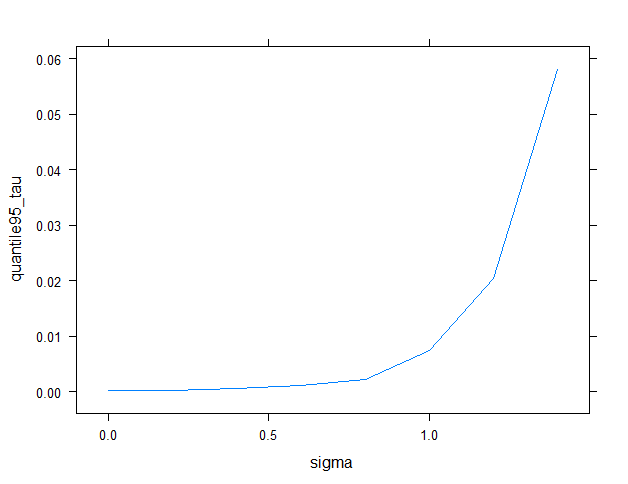
\includegraphics[width = 4.5in]{q95_tau1}
	\end{center}
	\caption{Зависимость $95\%$ квантиля для $\tau(U_1, U_2)$ от значения $\sigma$ шума.}
	\label{fig:q95_tau1}
\end{figure}

Значение $\sigma = 1$ является очень большим для рассматриваемой длины ряда, т.е. выше него шум уже сложно отличить от колебательной составляющей. Это видно по рис.~\ref{fig:q95_tau1}: после $\sigma=1$ график резко пошел вверх. Так что стоит рассматривать результаты для $\sigma=1$.

Полученные результаты говорят, что примерным необходимым значением порога является значение $t_0 = 0.01$.
Это значение было использовано при программировании для значения по умолчанию. Но эксперименты с реальными данными говорят, что оптимальное значение порога может сильно колебаться.

\section{Сравнение с частотным методов идентифкации}
\label{sec:compare}
Проведем сравнение разработанного метода по регулярности углов с частотным методов из раздела \ref{sec:1d_pgram_method}.
Аналогично, как в разделе \ref{sec:tau_study} исследовали распределение меры $\tau$, исследуем распределение меры $\rho_{ij}$, заданной в \eqref{eq:rho_ij}, частотного метода на тех же самых рядах. 
Также проведем сравнение методов для случая серии однотипных рядов

\subsection{Исследование распределения меры для частотного метода}
\label{sec:per_study}

Будем использовать для моделирования те же ряды $\mathbb{S}$, $\mathbb{N}$ и $\mathbb{X}$ с элементами вида
\eqref{eq:series_S_N}, \eqref{eq:series_N_N}, \eqref{eq:series_X_N}, что и ранее в разделе \ref{sec:tau_study}.
$N = 99$, $L = 50$, моделировать будем $1000$ раз.

Исследуем распределение значений  меры $\rho_{1,2}$ для пары сингулярных векторов э-м гармоники $\mathbb{S}$ и для пары векторов шума $\mathbb{N}$, мера $\rho_{ij}$ определена в \eqref{eq:rho_ij}. Затем посмотрим на распределения  $\rho_{1,2}$ и  $\rho_{3,4}$ для ряда $\mathbb{X} = \mathbb{S} + \mathbb{N}$.

Рассматриваем $\alpha = 0.01$. Возьмем $\omega = 1/7$, т.е. $L\omega$ --- не целое.

Значения $\rho^{\mathbb{S}}_{1,2}$  для ряда $\mathbb{S}$ всегда будут одинаковыми и равными  $\rho^{\mathbb{S}}_{1,2} = 0.950$. Характеристики распределения $\rho^{\mathbb{N}}_{1,2}$ для ряда $\mathbb{N}$ для разных $\sigma$ представлены в таблице~\ref{tab:model_dist_pgram_sig2}.

\begin{table}[hhh!]
\caption{Распределение $\rho^{\mathbb{N}}_{1,2}$.}
\centering
\begin{tabular}{rrrrrrr}
  \hline
 & Min. & 1st Qu. & Median & Mean & 3rd Qu. & Max. \\
  \hline
$\sigma$ = 0.2 & 0.000 & 0.000 & 0.711 & 0.549 & 0.849 & 0.982 \\ 
  $\sigma$ = 0.4 & 0.000 & 0.000 & 0.662 & 0.498 & 0.833 & 0.982 \\ 
  $\sigma$ = 0.6 & 0.000 & 0.000 & 0.661 & 0.513 & 0.833 & 0.986 \\ 
  $\sigma$ = 0.8 & 0.000 & 0.000 & 0.677 & 0.525 & 0.841 & 0.987 \\ 
  $\sigma$ = 1 & 0.000 & 0.000 & 0.678 & 0.518 & 0.835 & 0.989 \\ 
   \hline
\end{tabular}
\label{tab:model_dist_pgram_sig2}
\end{table}

По таблице \ref{tab:model_dist_pgram_sig2} видно, что значение $\rho^{\mathbb{S}}_{1,2} = 0.950$ пересекается с распределением $\rho^{\mathbb{N}}_{1,2}$ для всех значений $\sigma$, так как 0.950 меньше максимума  распределения $\rho^{\mathbb{N}}_{1,2}$ во всех случаях.

Посмотрим теперь на распределения  $\rho^{\mathbb{X}}_{1,2}$ и  $\rho^{\mathbb{X}}_{3,4}$ для ряда $\mathbb{X} = \mathbb{S} + \mathbb{N}$, представленные в таблицах ~\ref{tab:model_dist_pgram_sig_noise2} и \ref{tab:model_dist_pgram_sig_noise22}.

\begin{table}[hhh!]
\caption{Распределение $\rho^{\mathbb{X}}_{1,2}$.}
\centering
\begin{tabular}{rrrrrrr}
  \hline
 & Min. & 1st Qu. & Median & Mean & 3rd Qu. & Max. \\
  \hline
$\sigma$ = 0.2 & 0.925 & 0.945 & 0.949 & 0.949 & 0.953 & 0.967 \\ 
  $\sigma$ = 0.4 & 0.885 & 0.938 & 0.947 & 0.946 & 0.955 & 0.981 \\ 
  $\sigma$ = 0.6 & 0.873 & 0.929 & 0.943 & 0.942 & 0.955 & 0.989 \\ 
  $\sigma$ = 0.8 & 0.807 & 0.921 & 0.940 & 0.937 & 0.956 & 0.990 \\ 
  $\sigma$ = 1 & 0.000 & 0.904 & 0.931 & 0.924 & 0.952 & 0.991 \\ 
   \hline
\end{tabular}
\label{tab:model_dist_pgram_sig_noise2}
\end{table}

\begin{table}[hhh!]
\caption{Распределение $\rho^{\mathbb{X}}_{3,4}$.}
\centering
\begin{tabular}{rrrrrrr}
  \hline
 & Min. & 1st Qu. & Median & Mean & 3rd Qu. & Max. \\
  \hline
$\sigma$ = 0.2 & 0.000 & 0.000 & 0.694 & 0.533 & 0.850 & 0.985 \\ 
  $\sigma$ = 0.4 & 0.000 & 0.000 & 0.689 & 0.516 & 0.837 & 0.986 \\ 
  $\sigma$ = 0.6 & 0.000 & 0.000 & 0.675 & 0.517 & 0.834 & 0.983 \\ 
  $\sigma$ = 0.8 & 0.000 & 0.000 & 0.686 & 0.517 & 0.837 & 0.992 \\ 
  $\sigma$ = 1 & 0.000 & 0.000 & 0.679 & 0.525 & 0.835 & 0.985 \\ 
   \hline
\end{tabular}
\label{tab:model_dist_pgram_sig_noise22}
\end{table}

Построим оценки плотностей распределений $\rho^{\mathbb{X}}_{1,2}$  и  $\rho^{\mathbb{X}}_{3,4}$  и посчитаем процент их пересечения. Результаты представлены в таблице~\ref{tab:model_dist_pgram_overlap22}. При большом значении шума распределения пересекаются на 22 процента.
В таблице также приведены результаты для $\tau$ на тех же реализациях рядов. Видим, что для метода идентификации по регулярности углов процент пересечения на порядок меньше, чем для частотного метода.
Т.е. для метода с $\tau$ значения для сигнала больше отстают от значений шума, чем для частотного метода.

\begin{table}[hhh!]
\caption{Процент пересечения оценок плотностей для распределений $\rho^{\mathbb{X}}_{1,2}$  и $\rho^{\mathbb{X}}_{3,4}$.}
\centering
\begin{tabular}{rrr}
  \hline
& overlap\_$\tau$& overlap\_$\rho$ \\
  \hline
$\sigma$ = 0.2 & 0.0004 & 0.042 \\ 
  $\sigma$ = 0.4 & 0.0012 & 0.087 \\ 
  $\sigma$ = 0.6 & 0.0033 & 0.129 \\ 
  $\sigma$ = 0.8 & 0.0104 & 0.169 \\ 
  $\sigma$ = 1 & 0.0623 & 0.230 \\ 
   \hline
\end{tabular}
\label{tab:model_dist_pgram_overlap22}
\end{table}

\subsection{Сравнение для случая серии однотипных рядов}
\label{sec:comp_tau1_pgram_many_same_series}
Как обычно, будем использовать для моделирования ряды $\mathbb{S}$, $\mathbb{N}$ и $\mathbb{X}$ с элементами вида
\eqref{eq:series_S_N}, \eqref{eq:series_N_N}, \eqref{eq:series_X_N}, что и ранее в разделе \ref{sec:tau_study}.
$N = 99$, $L = 50$, моделировать будем $1000$ раз.

Цель автоматической идентификации идентифицировать так же, как визуальная.
Поэтому сравним методы следующим способом.
Будем моделировать э-м гармонику $\mathbb{S}$ и шум $\mathbb{N}$ 
c $\sigma = 0.2, 0.4, 0.6, 0.8, 1$, $\alpha = 0, 0.01$, $\omega = 1/7$ ($L\omega$ --- не целое).
Для фиксированных значений параметров $\alpha$, $\omega$, $\sigma$ будем моделировать ряд $\mathbb{X} = \mathbb{S} + \mathbb{N}$. Будем называться <<визуальной идентификации>> восстановление по первым двум компонентам.

Пусть $\mathbb{X}^{(1)}$ и $\mathbb{X}^{(2)}$ --- две реализации ряда $\mathbb{X}$.
Пусть $\mathbb{S}^{(V,1)}$ и  $\mathbb{S}^{(V,2)}$ --- ряды, восстановленные по рядам $\mathbb{X}^{(1)}$ и $\mathbb{X}^{(2)}$ <<визуальной идентификацией>>.


Обозначаем значение порога для метода с $\tau$ через $t_0$, а для частотного метода через $\rho_0$. 
Пусть $\mathbb{S}^{(A,1,\varepsilon)}$ и  $\mathbb{S}^{(A,1, \rho_0)}$ --- ряды, восстановленные по ряду $\mathbb{X}^{(1)}$  с помощью алгоритмов автоматической идентификации со значениями порогов $t_0$ и $\rho_0$ соответственно.
Также обозначим множество значений $T = \{0,0.01,0.02,\ldots, 0.99,1\}$, т.е. числа от $0$ до $1$ с шагом $0.01$.

Находим значения порогов $t_0^{opt}$ и $\rho_0^{opt}$, решая следующие задачи минимизации.

\begin{gather*}
t_0^{opt} = \argmin_{t_0 \in T}{\left(\frac{1}{N}\sum_{k=0}^{N-1}{\left(s_k^{(V,1)} - s_k^{(A,1,t_0)}\right)}^2\right)}, \\
\rho_0^{opt} = \argmin_{\rho_0 \in T}{\left(\frac{1}{N}\sum_{k=0}^{N-1}{\left(s_k^{(V,1)} - s_k^{(A,1,\rho_0)}\right)}    ^2\right)}.
\end{gather*}

Далее, пусть  $\mathbb{S}^{(A,2,t^{opt})}$ и  $\mathbb{S}^{(A,2, \rho_0^{opt})}$ --- ряды, восстановленные по ряду $\mathbb{X}^{(2)}$  с помощью алгоритмов автоматической идентификации со значениями порогов $t_0^{opt}$ и $\rho_0^{opt}$ соответственно.

Посчитаем ошибки идентификации для этих рядов:
\begin{gather*}
E_{\tau} = \frac{1}{N}\sum_{k=0}^{N-1}{\left(s(k)^{(V,2)} - s(k)^{(A,2,t_0^{opt})}\right)^2}, \\
E_{\rho} = \frac{1}{N}\sum_{k=0}^{N-1}{\left(s(k)^{(V,2)} - s(k)^{(A,2,\rho_0^{opt})}\right)^2}.
\end{gather*}

Таким образом, мы посчитали оптимальные значения порогов для одной реализации ряда $\mathbb{X}$, и с помощью этих оптимальных значений порогов восстановили ряды по второй реализации, и посчитали ошибку идентификации для полученных рядов.

Повторим описанную процедуру $200$ раз и посчитаем среднее и медиану ошибок идентификации $E_{\tau}$ и $E_{\rho}$. Результаты для $\alpha = 0$, $\omega = 1/7$ представлены в таблице~\ref{tab:comp_tau1_pgram}. Результаты для $\alpha = 0.02$, $\omega = 1/7$ представлены в таблице~\ref{tab:comp_tau1_pgram2}.

\begin{table}[hhh!]
\centering
\caption{Сравнение алгоритмов при $\alpha = 0$, $\omega = 1/7$.}
\begin{tabular}{rrrrr}
  \hline
 & mean\_$\tau$ & mean\_$\rho$ & median\_$\tau$ & median\_$\rho$ \\
  \hline
$\sigma$ = 0.2 & 0.0042 & 0.040 & 0 & 0.0028 \\ 
  $\sigma$ = 0.4 & 0.0156 & 0.064 & 0 & 0.0046 \\ 
  $\sigma$ = 0.6 & 0.0444 & 0.100 & 0 & 0.0342 \\ 
  $\sigma$ = 0.8 & 0.1012 & 0.151 & 0 & 0.0656 \\ 
  $\sigma$ = 1 & 0.1224 & 0.183 & 0 & 0.1179 \\ 
   \hline
\end{tabular}
\label{tab:comp_tau1_pgram}
\end{table}

\begin{table}[hhh!]
\centering
\caption{Сравнение алгоритмов при $\alpha = 0.02$, $\omega = 1/7$.}
\begin{tabular}{rrrrr}
  \hline
 & mean\_$\tau$ & mean\_$\rho$ & median\_$\tau$ & median\_$\rho$ \\
  \hline
$\sigma$ = 0.2 & 0.0003 & 0.050 & 0 & 0.0010 \\ 
  $\sigma$ = 0.4 & 0.0010 & 0.080 & 0 & 0.0020 \\ 
  $\sigma$ = 0.6 & 0.0082 & 0.103 & 0 & 0.0170 \\ 
  $\sigma$ = 0.8 & 0.0549 & 0.185 & 0 & 0.0655 \\ 
  $\sigma$ = 1 & 0.1917 & 0.239 & 0 & 0.1554 \\ 
   \hline
\end{tabular}
\label{tab:comp_tau1_pgram2}
\end{table}

Из таблиц \ref{tab:comp_tau1_pgram} и \ref{tab:comp_tau1_pgram2} можно сделать следующие выводы. Во-первых, для всех значений $\alpha$ и $\sigma$ метод идентификации по регулярности углов с мерой $\tau$ дает на порядок меньшие ошибки, чем частотный метод с мерой $\rho$, это подтверждает результаты таблицы \ref{tab:model_dist_pgram_overlap22}. Во-вторых, оба метода дают примерно одинаковые результаты для немодулированной  ($\alpha = 0$) и модулированной гармоник ($\alpha=0.02$). Для метода идентификации по регулярности углов такой результат подтверждается теорией, так как мера $\tau$ не зависит от $\alpha$. Для частотного метода такой результат неожиданен, так как метод основан на периодограмме сингулярных векторов, а для модулированной гармоники происходит <<растекание>> периодограммы. Результат можно объяснить тем фактом, что для частотного метода в алгоритме учитывается возможное растекание, и 
в качестве ключевой меры $\rho$, задаваемая формулой \eqref{eq:rho_ij}, берется сумма двух соседних значений периодограммы.



\chapter{Обобщения методов автоматической идентификации для разных вариантов SSA}
\label{sec:all_methods}

В данной главе приведем обобщения некоторых из методов из глав \ref{sec:1d_methods} и \ref{sec:tau1} для других типов объекта $\mathbb{X}$ и вариантов метода SSA. 

Сначала будет описано обобщение кластерного метода группировки из раздела \ref{sec:1D_wcor}, реализуемого алгоритмом \ref{alg:wcor}, сразу для всех вариантов SSA.
Затем отдельно для CSSA и MSSA будет приведено обобщение метода низких частот из раздела \ref{sec:1d_freq_method}, частотного метода для колебательной составляющей из раздела \ref{sec:1d_pgram_method} и метода идентификации колебательной составляющей по регулярности углов из главы \ref{sec:tau1}.
Для 2S-SSA обобщим только метод низких частот.

\section{Кластерный метод группировки}
В разделе \ref{sec:sep} приведены общие для всех типов объекта $\mathbb{X}$ определения w-корреляции и матрицы w-корреляций. Поэтому кластерный метод группировки и его алгоритм \ref{alg:wcor}, приведенные в разделе \ref{sec:1D_wcor}, одинаковы для всех типов объекта $\mathbb{X}$.

\section{Обобщения для CSSA}
Рассматриваем комплекснозначный временной ряд длины $N$: $\mathbb{X}=\mathbb{X}^{(1)} + \I \,\mathbb{X}^{(2)}$, $\mathbb{X}^{(k)}= \left(x^{(k)}(1),\ldots,x^{(k)}(N)\right)$, $k=1,2$, $x^{(k)}(i) \in \mathsf{R}$.

Комплексные временные ряды --- это искусственная вещь, в реальных задачах такие почти не встречается, за исключением комплексной экспоненты, т.е. э-м гармоники \eqref{eq:complex_exmodgarm} c $a=b$ и $|\phi_1 - \phi_2| = \pi/2 \,\,(\mod \pi)$. Пример, в котором возникают комплексные экспоненты, будет приведен далее в разделе \ref{sec:use_cssa}.

Таким образом, при идентификации комплексной колебательной составляющей наша главная цель --- идентифицировать гармоники ранга 1 с $a=b$ и $|\phi_1 - \phi_2| = \pi/2 \,\,(\mod \pi)$.
Частотный метод из раздела \ref{sec:1d_pgram_method} будет обобщен именно для этого случая. Для метода идентификации по регулярности углов из раздела \ref{sec:tau1} также приведем обобщение для э-м гармоник ранга 2 с $\omega \not = 0.5$; как говорилось в главе \ref{sec:tau1}, для $\omega=0.5$ метод по регулярности углов не работает. 

Из общего вида алгоритма SSA, описанного в разделе \ref{sec:ssa_alg}, видим, что в CSSA и левые и правые сингулярные вектора и восстановленные ряды являются комплексными, значит, к ним можно применять алгоритмы равнозначно.

Еще одна важная особенность CSSA: сингулярные вектора определяются с точностью до комплексного поворота, т.е. умножения на $e^{2\I\pi t}$, где $0 \leqslant t<1$. 
Рассматриваемые ниже меры часто будут зависеть отдельно от мнимой или вещественной частей сингулярного вектора.
Поэтому надо исследовать вопрос, как меняются вещественная и мнимая части вектора при комплексном повороте.
В случае колебательной составляющей, при умножении комплексной экспоненты (комплексной э-м гармоники ранга 1) на $e^{2\I\pi t}$ меняется только ее фаза, это не влияет на рассматриваемые меры.
В случае комплексной э-м гармоники ранга 2 (она будет идентифицироваться только в методе идентификации по регулярности углов) в методе учитывается эта особенность сингулярных векторов и подбирается нужный поворот. 
В случае тренда 
при умножении какого-то комплексного вектора на  $e^{2\I\pi t}$ могут поменяться значения вещественной и мнимой частей и частотный состав, поэтому, рекомендуется использовать вариант с восстановленными рядами, но будут описаны варианты алгоритма и для сингулярных векторов.


\subsection{Метод низких частот для идентификации тренда}
\label{sec:freq_method_cssa}
Обобщим алгоритм \ref{alg:freq1d} идентификации тренда из раздела \ref{sec:1d_freq_method} на случай комплексного ряда. 
Обобщение для комплексного случая также, как алгоритм \ref{alg:freq1d}, будет работать и для элементарных восстановленных рядов, и для левых, и для правых сингулярных векторов.

Предлагается алгоритм \ref{alg:freqcssa}, похожий на алгоритм \ref{alg:freq1d} метода низких частот  для 1D-SSA, но в котором в отличие от алгоритма \ref{alg:freq1d} на первом шаге будем вычислять меру отдельно для мнимой и вещественной частей $\mathbb{Y}_i$ и брать из них максимальную для использования на втором шаге алгоритма. 
Берется именно максимум, а не, например, среднее, потому что если для какой-то компоненты $\mathbb{Y}_i$ вещественная часть, соответствующая ряду $\mathbb{S}_1$, относится к тренду, а мнимая часть, соответствующая ряду $\mathbb{S}_2$, не относится, то среднее дало бы маленькое значение меры, которое могло бы не превзойти порог $T_0$.

\begin{algorithm}[!hhh]
\caption{CSSA. Метод низких частот для тренда}
\label{alg:freqcssa}
\begin{algorithmic}[1]
\REQUIRE На вход поступают данные и параметры.
\begin{enumerate}
\item \textbf{Данные}: группа индексов $I \in \{1,\ldots,d\}$; значение  $0 \leqslant  \omega \leqslant 0.5$; ряды $\mathbb{Y}_i$, $i \in I$: левые сингулярные вектора,
правые сингулярные вектора или элементарные восстановленные ряды.
\item \textbf{Параметры}: порог $0 \leqslant T_0 \leqslant 1$.
\end{enumerate}
\ENSURE Группа индексов компонент $J \subset I$, относящихся к тренду.
\STATE  Для каждого ряда $\mathbb{Y}_i = \mathbb{Y}^{(1)}_i + \I \mathbb{Y}^{(2)}_i $, $i \in I$, вычисляем значения $T(\mathbb{Y}^{(1)}_i; \omega)$ и $T(\mathbb{Y}^{(2)}_i; \omega)$ с помощью \eqref{eq:T_measure}. $T_m := \max \{T(\mathbb{Y}^{(1)}_i; \omega); T(\mathbb{Y}^{(2)}_i; \omega)\}$.
\STATE $J$ --- группа индексов $i \in I$, таких что $T_m \geqslant T_0$.
\end{algorithmic}
\end{algorithm}

Как уже говорилось выше в случае CSSA в методе низких частот в качестве входных данных рекомендуется использовать элементарные восстановленные ряды. 

\subsection{Частотный метод идентификации колебательной составляющей}
\label{sec:freq_cssa}
Как мы знаем, колебательная составляющая является суммой э-м гармоник.
Согласно разделу \ref{sec:cssa_theory} главы \ref{sec:ssa_theory} элементы комплекснозначного э.-м. гармонического ряда $\mathbb{S}$ имеют вид \eqref{eq:complex_exmodgarm}.

Из утверждения \ref{th:cssa_ex_mod_im_vec} известно, для ряда $\mathbb{S}$ ранг ряда $d$ может равняться или $2$, или $1$, т.е. ему может соответствовать либо один, либо два левых сингулярных вектора. 

Как уже отмечали в начале раздела, будем идентифицировать гармоники $\mathbb{S}$ ранга 1 c $a=b$ и $|\phi_1 - \phi_2| = \pi/2 \,\,(\mod \pi)$.
 Из утверждения \ref{th:cssa_ex_mod_im_vec} раздела \ref{sec:cssa_theory} следует, что в случае $a=b$ и $|\phi_1 - \phi_2| = \pi/2 \,\,(\mod \pi)$ единственный сингулярный вектор $U_1$ ряда $\mathbb{S}$ имеет вид \eqref{eq:vid_d1}, это сумма синуса и косинуса с одинаковой частотой $\omega$.

Частотный метод для 1D-SSA имел два этапа, на каждом этапе сингулярный вектор $U_j$ участвовал только в значении его периодограммы $\Pi_{U_j}^L(k/L)$.

Ввиду вышесказанного алгоритм идентификации комплексной э-м гармоники следующий. Применяем алгоритм, как для 1D-SSA, только вместо последовательной пары $U_i, U_{i+1}$ сингулярных векторов берем пару векторов, соответствующих мнимой и вещественной части  комплексного вектора $U_i$.
Так как вектора, к которым применяем частотный метод, должны иметь норму 1, то вместо векторов $U_i$ рассмотрим вектора: 
\begin{gather*}
\widehat{U}_{i} := \widehat{U}^{(\RE)}_{i} +  \I \,\widehat{U}^{(\IM)}_{i},
\end{gather*}
где
\begin{gather*} 
\widehat{U}^{(\RE)}_{i}:= \frac{\RE(U_i)}{\|\RE(U_i) \|}, \quad \widehat{U}^{(\IM)}_{i}:= \frac{\IM(U_i)}{\|\IM(U_i) \|}.
\end{gather*}
т.е $\| \widehat{U}^{(\RE)}_{i}\| = \| \widehat{U}^{(\IM)}_{i} \| = 1$. 

 
Таким образом, введем следующие обозначения.  
\begin{gather} \label{eq:I_1_P_cssa}
I_1^{(\mathbb{P})} = \{ i: \quad \theta_1 \theta_2 >0, \quad L |\theta_i^{(\RE)} - \theta_{i}^{(\IM)}| \leqslant s_0, \quad 1 \leqslant i \leqslant в  \},
\end{gather}
где $\theta_i^{(\RE)} = \argmax_{0 < k \leqslant L/2} \{\Pi_{\widehat{U}^{(\RE)}_{i}}^L(k/L)\}$, $\theta_{i}^{(\IM)} = \argmax_{0 < k \leqslant L/2} \{\Pi_{\widehat{U}^{(\IM)}_{i}}^L(k/L)\}$ --- аргументы максимума периодограмм $\Pi_{\widehat{U}^{(\RE)}_{i}}^L$ и $\Pi_{\widehat{U}^{(\IM)}_{i}}^L$ вещественной и мнимой частей сингулярного вектора $\widehat{U}_i$ соответственно.
\begin{gather} \label{eq:rho_i_cssa}
\rho_{i} := \max_{0 < k \leqslant L/2}{\left(\rho_{\{\widehat{U}^{(\RE)}_{i},\widehat{U}^{(\IM)}_{i}\}}(k/L) + \rho_{\{\widehat{U}^{(\RE)}_{i},\widehat{U}^{(\IM)}_{i}\}}((k+1)/L)\right)},
\end{gather}
определение \ref{def:rho} меры $\rho_A$ дано в разделе \ref{sec:1d_pgram_method}.
\begin{gather} \label{eq:pgram_I_p_cssa}
I^{(\mathbb{P})} = \{ i \in I_1^{(\mathbb{P})}: \rho_{i} \geqslant\rho_0 \}.
\end{gather}
Ниже приведем алгоритм \ref{alg:cssa_pgram} частотного метода для CSSA.
\begin{algorithm}[!hhh]
\caption{СSSA. Частотный метод для колебательной составляющей}
\label{alg:cssa_pgram}
\begin{algorithmic}[1]
\REQUIRE На вход поступают данные и параметры.
\begin{enumerate}
\item \textbf{Данные}: левые сингулярные вектора $\{U_i\}_{i=1}^{d}$.
\item \textbf{Параметры}: параметр $s_0 \in \mathsf{Z}_{+}$, порог $\rho_0 \in [0,1]$.
\end{enumerate}
\ENSURE Группа индексов компонент $I^{(\mathbb{P})}$, относящихся к колебательной составляющей.
\STATE  По $\{U_i\}_{i=1}^{d}$ получаем группу индексов $I_1^{(\mathbb{P})}$ с помощью $s_0$ и \eqref{eq:I_1_P_cssa}.
\STATE Получаем группу $I^{(\mathbb{P})}$ по $\{\widehat{U}_j\}_{j \in I_1^{(\mathbb{P})}}$ и $\rho_0$ с помощью \eqref{eq:pgram_I_p_cssa}.
\end{algorithmic}
\end{algorithm}


\subsection{Метод идентификации колебательной составляющей по регулярности углов}
\label{sec:tau_cssa}
Как уже отмечалось ранее в начале раздела про обобщения CSSA и в главе \ref{sec:tau1} для данного метода, мы не рассматриваем случай $\omega=0.5$.

Описание метода идентификации колебательной составляющей по регулярности углов из главы \ref{sec:tau1} для комплексных э-м гармоник, основанного на специальной мере $\tau$, задаваемой формулой \eqref{eq:tau1}, было приведено в моей бакалаврской работе \cite{Zhornikova2016}. Опишем метод и приведем его алгоритм.

Для $d=2$ вид левых сингулярных векторов для комплексной гармоники приведен в формулах \eqref{eq:uuu1} и \eqref{eq:uuu2} в разделе \ref{sec:cssa_theory}.
Из утверждения \ref{th:th_tau_cssa} этого же раздела следует, что при определенных условиях всегда существует один поворот $2\pi t$ или последовательность поворотов $2\pi t = 2\pi t_L$ и для мнимой, и для вещественной частей вектора $U_2$, приводящий к равенствам
\begin{gather*}
\lim_{L \rightarrow \infty}({\tau} (\RE U_1, \RE e^{\I 2\pi t} U_2) + {\tau} (\IM U_1, \IM e^{\I 2\pi t} U_2))= 0.
\end{gather*}
Поэтому в случае $d=2$ для пары $(U_i,\,U_j)$, $i<j$, решается оптимизационная задача
\begin{gather} \label{eq:cssa_tau_opt}
 \tilde{\tau}(\RE U_i, \RE e^{\I 2\pi t} U_j) + \tilde{\tau}(\IM U_i, \IM e^{\I 2\pi t} U_j) \longrightarrow \min_{t},
\end{gather}
где $\tilde{\tau}$ задано в формуле \eqref{eq:tau_norm}.
На $t_{i,j}$ достигается минимум, $\tau_{i,j}$ --- минимальное значение.
Отбираем пары индексов $i$, $j$ векторов $\left(U_i, \,\,e^{\mathrm{i} 2\pi t_{i,j}}U_j\right)$, у которых значение меры $\tau_{i,j}$
меньше заданного порога $t_0$, или берем фиксированное число э-м гармоник, если оно задано, с наименьшими значениями $\tau_{i,j}$.

Для $d=1$ единственный сингулярный вектор имеет вид \eqref{eq:vid_d1} и, согласно  утверждению \ref{th:th_tau_cssa_d1} раздела \ref{sec:cssa_theory} в этом случае стоит рассматривать значения $\tilde{\tau}(\RE U_i, \IM U_i)$.
Отбираем индексы $i$ векторов $U_i$, у которых значение меры $\tilde{\tau}(\RE U_i, \IM U_i)$
меньше заданного порога $t_0$,
или берем фиксированное число э-м гармоник, если оно задано, с наименьшими значениями $\tilde{\tau}(\RE U_i, \IM U_i)$.

Как и в вещественном случае метод имеет две модификации. Алгоритм \ref{alg:cssatau_2} с двумя варианта критерия остановки представлен ниже. 

\begin{algorithm}[!hhh]
\caption{CSSA. Метод идентификации по регулярности углов для колебательной составляющей, число э-м гармоник известно}
\label{alg:cssatau_2}
\begin{algorithmic}[1]
\REQUIRE На вход поступают данные и параметры.
\begin{enumerate}
\item \textbf{Данные}: число компонент $r$; левые сингулярные вектора $\{U_j\}_{j=1}^{r}$.\\
\item \textbf{Параметры}:  количество $m_1$ э-м гармоник ранга 1 и количество $m_2$ э-м гармоник ранга 2, $m_1 + 2 m_2 \leqslant r$; либо порог $t_0 \geqslant 0$, в зависимости от критерия остановки.
\end{enumerate}
\ENSURE Группа индексов компонент $J$, относящихся к колебательной составляющей.
\STATE По $\{U_i\}_{i=1}^{r}$ вычисляем и упорядочиваем по возрастанию значения $\tilde{\tau}(\RE U_j, \IM U_j)$, $j=1,\ldots, r$ с помощью \eqref{eq:tau_norm}; полученные значения:  $\tau_1^{(1)}, \ldots, \tau_{r}^{(1)}$.
\STATE Идем по множеству $\tau_l^{(1)}$, $l=1,\ldots,r$
\begin{enumerate}
\item либо пока $l < m_1$;
\item либо пока $\tau_l^{(1)} < t_0$.
\end{enumerate}
$l_0$ --- момент остановки.
\STATE $J_1$ --- индексы $j$ сингулярных векторов $U_j$, участвующих в вычислении  значений $\tau_1^{(1)}, \ldots, \tau_{l_0 - 1}^{(1)}$.
\STATE Для пары $(U_i,\,U_j)$, $i<j$, $i,j \not \in J_1$, решается оптимизационная задача \eqref{eq:cssa_tau_opt}.
На $t_{i,j}$ достигается минимум, $\tau_{i,j}$ --- минимальное значение;\\
$\tau_1^{(2)}, \ldots, \tau_{d(d-1)}^{(2)}$ --- отсортированные значения $\tau_{i,j}$, $i,j=1,\ldots, d$, $i \not = j$.
\STATE Идем по множеству $\tau_k^{(2)}$, $k=1,\ldots,r$
\begin{enumerate}
\item либо пока $k < m_2$;
\item либо пока $\tau_k^{(2)} < t_0$.
\end{enumerate}
$k_0$ --- момент остановки.
\STATE $J_2$ --- индексы $i$, $j$ сингулярных векторов $U_i$ и $U_{j}$, участвующих в вычислении  значений $\tau_1^{(2)}, \ldots, \tau_{k_0 - 1}^{(2)}$.
\STATE $J = J_1 \cup J_2$.
\end{algorithmic}
\end{algorithm}

\begin{remark}
По утверждению \ref{th:cssa_num} собственные числа комплексной э-м гармоники не являются равными, поэтому в случае CSSA, чтобы найти пары сингулярных векторов, соответствующие гармонике ранга 2, недостаточно рассматривать последовательные пары, нужно рассматривать всевозможные пары векторов.
\end{remark}

\begin{remark}
Аналогично, как в вещественном случае, на вход алгоритма могут подаваться не только первые $r$ сингулярных векторов. Может подавать любое подмножество из множества $\{U_j\}_{j=1}^{d}$, так как в комплексном случае мы рассматриваем все пары векторов, а не только последовательные.
\end{remark}

\begin{remark}
По описанному алгоритму \ref{alg:cssatau_2} в итоговое множество индексов $J_1$ некоторые индексы могут попасть несколько раз. 
В комплексном случае также можно делать дополнительный отбор и выбирать пару с наименьшим значением меры из двух пар с одинаковым вектором, но это не было описано в алгоритме и реализовано при программировании ввиду высокой трудоемкости.
\end{remark}

Проблемы выбора порога в комплексном случае аналогичны случаю 1D-SSA. 

\section{Обобщения для MSSA}

Рассматриваем многомерный временной ряд $\mathbb{X}= \left(\mathbb{X}^{(1)}, \ldots,\mathbb{X}^{(s)}\right)$,\\ $\mathbb{X}^{(p)}= \left(x^{(p)}(1),\ldots,x^{(p)}(N_p)\right)$, $p=1,\ldots,s$, $x^{(p)}(i) \in \mathsf{R}$. 

Основная особенность MSSA, в отличие от вещественного или комплексного случая, состоит в том, что все три вида объектов: элементарные восстановленные ряды, левые сингулярные вектора и правые сингулярные вектора, имеют разную структуру.

Из описания алгоритма MSSA, приведенного в разделе \ref{sec:ssa_alg}, следует, что восстановленные ряды имеют такое же вид, как и исходный многомерный ряд, т.е. тоже являются многомерными рядами (или системой временных рядов). 

Из утверждения \ref{th:mssa_vec} для MSSA левые сингулярные вектора --- это одномерные вещественнозначные временные ряды
 длины $L$. 
Они описывают общую структуру рядов $\mathbb{X}^{(1)}, \ldots, \mathbb{X}^{(s)}$ (пространств столбцов траекторных матриц). Они имеют ту же форму, как сингулярные вектора для одного ряда.
 
 Правые сингулярные вектора также являются одномерными вещественнозначными временными рядами,  они описывают общую структуру пространства строк траекторных матриц, каждая из которых описывается элементами всех рядов $\mathbb{X}^{(1)}, \ldots, \mathbb{X}^{(s)}$, а не только одного.
 

Введем для правых сингулярных векторов $V_i$ следующие обозначения: 
\begin{gather} \label{eq:V_mssa}
{V}_{i} = \left({V}_i^{(1)}, \ldots, {V}_i^{(s)}\right), 
\end{gather}
где $V_i^{(1)}$ --- первые $K_1$ элементов вектора ${V}_{i}$,  $V_i^{(2)}$, --- вторые $K_2$ элементов вектора ${V}_{i}$ и, так далее, $V_i^{(s)}$ --- последние $K_s$ элементов вектора ${V}_{i}$, $0 \leqslant i \leqslant d$. 

Ввиду вышесказанного, для MSSA алгоритмы будут иметь разные модификации для разных вариантов входных объектов. Разные модификации алгоритмов могут давать разные результаты, например, в случае применения алгоритма к правым сингулярным векторам, в отличие от левых сингулярных векторов, в каждом векторе учитывается каждый из $s$ рядов отдельно.  
 

\subsection{Метод низких частот для идентификации тренда}
\label{sec:freq_method_mssa}

Обобщим алгоритм \ref{alg:freq1d} идентификации тренда из раздела \ref{sec:1d_freq_method} на случай многомерного ряда. Алгоритм \ref{alg:freq1d} можно было применять либо к левым или правым сингулярным векторам, либо к элементарным восстановленным рядам. 

Как уже говорилось, в MSSA левые сингулярные вектора являются одномерными вещественнозначными временными рядами длины $L$ и имеют ту же форму, как сингулярные вектора для одного ряда. Т.е. левые сингулярные вектора имеют такой же вид, как в случае 1D-SSA, к ним можно применить алгоритм \ref{alg:freq1d} метода низких частот точно так же. Алгоритм \ref{alg:freqmssa_1} для этого случая приведен ниже.

Правые сингулярные вектора являются одномерными вещественнозначными временными рядами длины $K$ и представимы в виде \eqref{eq:V_mssa}. К частям ${V}_i^{(1)}, \ldots, {V}_i^{(s)}$ правого сингулярного вектора $V_i$ мы можем применить метод низких частот, аналогично, как в комплексном случае применяли к мнимой и вещественной частям вектора: считаем меру \eqref{eq:T_measure} для каждой части ${V}_i^{(1)}, \ldots, {V}_i^{(s)}$ вектора $V_i$, и берем максимум. Предлагаемый алгоритм \ref{alg:freqmssa_2} формально описан ниже.

Элементарные восстановленные ряды в случае MSSA являются многомерными временными рядами. Идея применения метода низких частот к ним такая же, как в комплексном случае или для правых сингулярных векторов: на первом шаге для каждого из $s$ рядов считаем меру по формуле \eqref{eq:T_measure} и берем максимальное значение этой меры для использования на втором шаге.
Этот вариант метода тоже задается алгоритмом  \ref{alg:freqmssa_2}, только в качестве входных данные берутся не сингулярные вектора, а элементарные восстановленные ряды.

 \begin{algorithm}[!hhh]
\caption{MSSA. Метод низких частот для тренда: вариант с левыми сингулярными векторами}
\label{alg:freqmssa_1}
\begin{algorithmic}[1]
\REQUIRE На вход поступают данные и параметры.
\begin{enumerate}
\item \textbf{Данные}: группа индексов $I \in \{1,\ldots,d\}$; значение  $0 \leqslant  \omega \leqslant 0.5$; левые сингулярные вектора $U_i$, $i \in I$.
\item \textbf{Параметры}: порог $0 \leqslant T_0 \leqslant 1$.
\end{enumerate}
\ENSURE Группа индексов компонент $J \subset I$, относящихся к тренду.
\STATE  Для каждого вектора $U_i$, $i \in I$, вычисляем значение $T(U_i; \omega)$ с помощью  \eqref{eq:T_measure}.
\STATE $J$ --- группа индексов $i \in I$, таких что $T(U_i; \omega) \geqslant T_0$
\end{algorithmic}
\end{algorithm}

\begin{algorithm}[!hhh]
\caption{MSSA. Метод низких частот для тренда: вариант с правыми сингулярными векторами или элементарными восстановленными рядами}
\label{alg:freqmssa_2}
\begin{algorithmic}[1]
\REQUIRE На вход поступают данные и параметры.
\begin{enumerate}
\item \textbf{Данные}: группа индексов $I \in \{1,\ldots,d\}$; значение  $0 \leqslant  \omega \leqslant 0.5$; ряды $\mathbb{Y}_i$, $i \in I$: 
правые сингулярные вектора или элементарные восстановленные ряды.
\item \textbf{Параметры}: порог $0 \leqslant T_0 \leqslant 1$.
\end{enumerate}
\ENSURE Группа индексов компонент $J \subset I$, относящихся к тренду.
\STATE  Для каждого ряда $\mathbb{Y}_{i} = (\mathbb{Y}_i^{(1)}, \ldots, \mathbb{Y}_i^{(s)})$, $i \in I$, вычисляем значения $T(\mathbb{Y}_i^{(1)}; \omega), \ldots,
T(\mathbb{Y}_i^{(s)}; \omega)$ с помощью  \eqref{eq:T_measure}. $T_m := \max \{T(\mathbb{Y}_i^{(1)}; \omega); \ldots;
T(\mathbb{Y}_i^{(s)}; \omega)\}$.
\STATE $J$ --- группа индексов $i \in I$, таких что $T_m \geqslant T_0$.
\end{algorithmic}
\end{algorithm}


\newpage
\subsection{Частотный метод идентификации колебательной составляющей}
Колебательная составляющая является суммой э-м гармоник.
Согласно разделу \ref{sec:mssa_theory} элементы многомерного э.-м. гармонического ряда $\mathbb{S}$ имеют вид \eqref{eq:em_mssa}.

В MSSA левые сингулярные вектора являются одномерными вещественнозначными временными рядами длины $L$ и имеют ту же форму, как сингулярные вектора для одного ряда. Поэтому к ним частотный метод можно применить точно так же, как в случае 1D-SSA. Ниже приведем алгоритм \ref{alg:mssa_pgram_1} частотного метода для MSSA и левых сингулярных векторов.

\begin{algorithm}[!hhh]
\caption{MSSA. Частотный метод для колебательной составляющей: вариант с левыми сингулярными векторами}
\label{alg:mssa_pgram_1}
\begin{algorithmic}[1]
\REQUIRE На вход поступают данные и параметры.
\begin{enumerate}
\item \textbf{Данные}: левые сингулярные вектора $\{U_i\}_{i=1}^{d}$.
\item \textbf{Параметры}: параметр $s_0 \in \mathsf{Z}_{+}$, порог $\rho_0 \in [0,1]$.
\end{enumerate}
\ENSURE Группа индексов компонент $I^{(\mathbb{P})}$, относящихся к колебательной составляющей.
\STATE  По $\{U_i\}_{i=1}^{d}$ получаем группу индексов $I_1^{(\mathbb{P})}$ с помощью $s_0$ и \eqref{eq:I_1_P} и группу индексов $I_2^{(\mathbb{P})}$ с помощью $s_0$ и \eqref{eq:I_2_P}.
\STATE Получаем группу индексов $I^{(\mathbb{P})}$ по $\{U_j\}_{j \in I_1^{(\mathbb{P})} \cup I_2^{(\mathbb{P})}}$ и $\rho_0$ с помощью \eqref{eq:pgram_I_p}.
\end{algorithmic}
\end{algorithm}

Как уже несколько раз упоминалось, правые сингулярные вектора $V_i$
 имеют вид \eqref{eq:V_mssa}.
Так как вектора, к которым применяем частотный метод, должны иметь норму 1, то вместе векторов $V_i$ рассмотрим вектора: 
\begin{gather*}
\widehat{V}_{i} := \left(\widehat{V}_i^{(1)}, \ldots, \widehat{V}_i^{(s)}\right),
\end{gather*}
где
\begin{gather*}
\widehat{V}_i^{(p)} := \frac{V_i^{(p)}}{\|V_i^{(p)} \|},
\end{gather*}
т.е. $\| \widehat{V}_i^{(p)} \| = 1$. 

На первом этапе метода будет обирать множества индексов $I_{1,p}^{(\mathbb{P})}$, $p=1,\ldots,s$:
\begin{gather} \label{eq:I_1_P_mssa}
I_{1,p}^{(\mathbb{P})} = \{ i: \quad \theta_{i}^{(p)} \theta_{i+1} ^{(p)} >0, \quad L |\theta_i^{(p)} - \theta_{i+1}^{(p)}| \leqslant s_0, \quad 1 \leqslant i \leqslant d -1  \},
\end{gather}
где $\theta_i^{(p)} = \argmax_{0 < k \leqslant K_p/2} \{\Pi_{\widehat{V}_i^{(p)}}^{K_p}(k/{K_p})\}$, $p=1,\ldots,s$.
Т.е. для каждого $p = 1,\ldots,s$
мы последовательно вычисляем множества $I_{1,p}^{(\mathbb{P})}$ для каждой пары векторов  $\widehat{V}_i^{(p)}$, $\widehat{V}_{i+1}^{(p)}$ длины $K_p$.

Аналогично каждый сингулярный вектор проверяется на соответствие гармонике с частотой 0.5:
\begin{gather} \label{eq:I_2_P_mssa}
I_{2,p}^{(\mathbb{P})} = \{i: \quad  {K_p} |\theta_{i}^{(p)} - 0.5 | \leqslant s_0, \quad 1 \leqslant i \leqslant d  \}.
\end{gather}
Далее определим общие индексы для второго этапа: $I_1^{(\mathbb{P})}$ --- объединение множества $\{ I_{1,p}^{(\mathbb{P})} \}_{p=1}^{s}$, $I_2^{(\mathbb{P})}$ --- объединение множества $\{ I_{2,p}^{(\mathbb{P})} \}_{p=1}^{s}$.

Для второго этапа введем определение
\begin{gather*}
\rho_{i,j} :=  \max_p \{ \max_{0 < k \leqslant {K_p}/2}{\left(\rho_{\{\widehat{V}_i^{(p)}, \widehat{V}_{j}^{(p)}\}}(k/{K_p}) + \rho_{\{\{\widehat{V}_i^{(p)}, \widehat{V}_{j}^{(p)}\}}((k+1)/{K_p})\right)}, p=1,\ldots, s
 \},
\end{gather*}
где $\widehat{V}_i^{(p)}, \widehat{V}_{j}^{(p)}$ --- вектора с индексами из множества индексов $I_1^{(\mathbb{P})}$ отобранных на первом этапе,
определение \ref{def:rho} меры $\rho_A$ дано в разделе \ref{sec:1d_pgram_method}.

Для идентификации компонент, относящихся к гармонике с частотой 0.5, мера имеет вид
\begin{gather*}
\rho_{i} :=  \max_p \{ \max_{0 \leqslant k \leqslant {K_p}/2}{\left(\rho_{\{\widehat{V}_i^{(p)}\}}(\lfloor {K_p}/2 \rfloor/{K_p}) + \rho_{\{\{\widehat{V}_i^{(p)}\}}((\lfloor {K_p}/2 \rfloor + 1)/{K_p})\right)}, p=1,\ldots, s
 \},
\end{gather*}
где $i \in I_2^{(\mathbb{P})}$.

Итоговым результатом частотного метода метода для MSSA и правых сингулярных векторов, реализуемого алгоритмом \ref{alg:mssa_pgram_2}, являются индексы 
\begin{gather} \label{eq:pgram_I_p_mssa_2}
I^{(\mathbb{P})} = \{ (i,j): \rho_{i,j} \geqslant\rho_0 \} \cup \{ i: \rho_{i} \geqslant\rho_0 \}.
\end{gather}


\begin{algorithm}[!hhh]
\caption{MSSA. Частотный метод для колебательной составляющей: вариант с правыми сингулярными векторами}
\label{alg:mssa_pgram_2}
\begin{algorithmic}[1]
\REQUIRE На вход поступают данные и параметры.
\begin{enumerate}
\item \textbf{Данные}: правые сингулярные вектора $\{V_i\}_{i=1}^{d}$.
\item \textbf{Параметры}: параметр $s_0 \in \mathsf{Z}_{+}$, порог $\rho_0 \in [0,1]$.
\end{enumerate}
\ENSURE Группа индексов компонент $I^{(\mathbb{P})}$, относящихся к колебательной составляющей.
\STATE  
По $\{V_i\}_{i=1}^{d}$ получаем группу индексов $I_{1,p}^{(\mathbb{P})}$, $p=1,\ldots,s$, с помощью $s_0$ и \eqref{eq:I_1_P_mssa} и группу индексов $I_{2,p}^{(\mathbb{P})}$, $p=1,\ldots,s$, с помощью $s_0$ и \eqref{eq:I_2_P_mssa};\\
$I_1^{(\mathbb{P})}$ --- объединение множеств $\{ I_{1,p}^{(\mathbb{P})} \}_{p=1}^{s}$, $I_2^{(\mathbb{P})}$ --- объединение множеств $\{ I_{2,p}^{(\mathbb{P})} \}_{p=1}^{s}$.
\STATE Получаем группу индексов $I^{(\mathbb{P})}$ по $\{V_j\}_{j \in I_1^{(\mathbb{P})} \cup I_2^{(\mathbb{P})}}$ и $\rho_0$ с помощью \eqref{eq:pgram_I_p_mssa_2}.
\end{algorithmic}
\end{algorithm}


\subsection{Метод идентификации колебательной составляющей по регулярности углов} 
Опять же, если мы рассматриваем левые сингулярные вектора, то алгоритм можно применить точно так же, как в случае 1D-SSA. Алгоритм \ref{alg:tau_mssa} для данного случая приведен ниже
\begin{algorithm}[!hhh]
\caption{MSSA. Метод идентификации по регулярности углов для колебательной составляющей: вариант с левыми сингулярными векторами}
\label{alg:tau_mssa}
\begin{algorithmic}[1]
\REQUIRE На вход поступают данные и параметры.
\begin{enumerate}
\item \textbf{Данные}: число компонент $r$; левые сингулярные вектора $\{U_j\}_{j=1}^{r}$.\\
\item \textbf{Параметры}: количество э-м гармоник $m \leqslant r/2$, либо порог $t_0 \geqslant 0$, в зависимости от критерия остановки.
\end{enumerate}
\ENSURE Группа индексов сингулярных векторов $J$, относящихся к колебательной составляющей.
\STATE По $\{U_i\}_{i=1}^{r}$ вычисляем и упорядочиваем по возрастанию значения $\tilde{\tau}(U_j, U_{j+1})$, $j=1,\ldots, r-1$ с помощью \eqref{eq:tau_norm}. 
При вычислении для каждого $j = 2,\ldots,r-1$ проверяем: если $\tilde{\tau}(U_j, U_{j+1}) < \tilde{\tau}(U_{j-1}, U_{j})$, то выкидываем из рассмотрения значение $\tilde{\tau}(U_{j-1}, U_{j})$; иначе выкидываем $\tilde{\tau}(U_j, U_{j+1})$.
 Полученные значения: $\tau_1, \ldots, \tau_{\lfloor r/2 \rfloor}$.
\STATE Два варианта критерия остановки. Идем по множеству $i=1,\ldots,\lfloor r/2 \rfloor$
\begin{enumerate}
\item либо пока $i < m$;
\item либо пока $\tau_i < t_0$.
\end{enumerate}
$i_0$ --- момент остановки.
\STATE $J$ --- индексы $j$, $j+1$ сингулярных векторов $U_j$ и $U_{j+1}$, участвующих в вычислении  значений $\tau_1, \ldots, \tau_{i_0 - 1}$.
\end{algorithmic}
\end{algorithm}

К правым сингулярным векторам метод можно применить аналогичным способом, как для частотного метода. 
Вычисляем значения $\tilde{\tau}(V_j^{(p)}, V_{j+1}^{(p)})$, $p=1,\ldots,s$, для последовательной пары правых сингулярных векторов $V_{j} = (V_j^{(1)}, \ldots, V_j^{(s)})$ и $V_{j+1} = (V_{j+1}^{(1)}, \ldots, V_{j+1}^{(s)})$, $j=1,\ldots,r-1$, вид которых определен формулой \eqref{eq:V_mssa}. Далее для каждого $j$ берем минимальное значение $\tilde{\tau}^{(\min)}(V_j, V_{j+1}) =\min_p \{ \tilde{\tau}(V_j^{(p)}, V_{j+1}^{(p)}), p=1,\ldots,s \}$, и к уже получившимся значениям $\tilde{\tau}^{(\min)}(V_j, V_{j+1})$ применяем стандартный алгоритм, как в одномерном случае. Получающийся алгоритм \ref{alg:tau_mssa_fac} приведен ниже.

\begin{algorithm}[!hhh]
\caption{MSSA. Метод идентификации по регулярности углов для колебательной составляющей: вариант с правыми сингулярными векторами}
\label{alg:tau_mssa_fac}
\begin{algorithmic}[1]
\REQUIRE На вход поступают данные и параметры.
\begin{enumerate}
\item \textbf{Данные}: число компонент $r$; правые сингулярные вектора $\{V_j\}_{j=1}^{r}$.\\
\item \textbf{Параметры}: количество э-м гармоник $m \leqslant r/2$, либо порог $t_0 \geqslant 0$, в зависимости от критерия остановки.
\end{enumerate}
\ENSURE Группа индексов сингулярных векторов $J$, относящихся к колебательной составляющей.
\STATE 
Для каждой пары векторов $V_{j} = (V_j^{(1)}, \ldots, V_j^{(s)})$ и $V_{j+1} = (V_{j+1}^{(1)}, \ldots, V_{j+1}^{(s)})$ 
вычисляем значения $\tilde{\tau}(V_j^{(p)}, V_{j+1}^{(p)})$ с помощью \eqref{eq:tau_norm}, $j=1,\ldots, r-1$, $p=1,\ldots,s$.
\STATE Вычисляем $\tilde{\tau}^{(\min)}(V_j, V_{j+1}) =\min_p \{ \tilde{\tau}(V_j^{(p)}, V_{j+1}^{(p)}), p=1,\ldots,s \}$.
\STATE Для каждого $j = 2,\ldots,r-1$ проверяем: если $\tilde{\tau}^{(\min)}(V_j, V_{j+1})< \tilde{\tau}^{(\min)}(V_{j-1}, V_{j})$, то выкидываем из рассмотрения значение $\tilde{\tau}^{(\min)}(V_{j-1}, V_{j})$; иначе выкидываем $\tilde{\tau}^{(\min)}(V_j, V_{j+1})$.
 Упорядочиваем полученные значения по возрастанию и получаем: $\tau_1, \ldots, \tau_{\lfloor r/2 \rfloor}$.
\STATE Два варианта критерия остановки. Идем по множеству $i=1,\ldots,\lfloor r/2 \rfloor$
\begin{enumerate}
\item либо пока $i < m$;
\item либо пока $\tau_i < t_0$.
\end{enumerate}
$i_0$ --- момент остановки.
\STATE $J$ --- индексы $j$, $j+1$ сингулярных векторов $V_j$ и $V_{j+1}$, участвующих в вычислении  значений $\tau_1, \ldots, \tau_{i_0 - 1}$.
\end{algorithmic}
\end{algorithm}


\newpage
\section{Обобщения для 2D-SSA}

Рассматриваем поле размера $N_x \times N_y$: $\mathbb{X}= \left(x(i,j) \right)_{i,j=1}^{N_x,N_y}$, $x(i,j) \in \mathsf{R}$.

Для 2D-SSA мы обобщим только метод низких частот, описанный алгоритмом \ref{alg:freq1d}, но так как в качестве тренда может выступать гармоника с очень маленькой частотой, то было проведено небольшое исследование свойств двумерных гармоник.

Согласно разделу \ref{sec:2d_ssa_theory} главы \ref{sec:ssa_theory} элементы двумерной гармоники $\mathbb{S}$ с частотами $\omega^{(X)}$, $\omega^{(Y)}$ имеют вид \eqref{eq:2d_cos_el},
где $1 \leqslant k \leqslant N_x$, $1 \leqslant l \leqslant N_y$, хотя бы один коэффициент из  группы $\{a,b,c,d\}$ не равен нулю и
$\omega^{(X)}, \omega^{(Y)} \in (0,0.5)$.

Колебательная составляющая  $\mathbb{H}$ --- это сумма какого-то числа $c$ двумерных гармоник. Элементы $\mathbb{H}$ имеют задаются формулой \eqref{eq:2d_cos},
где $1 \leqslant k \leqslant N_x$, $1 \leqslant l \leqslant N_y$, хотя бы один коэффициент из каждой группы $\{a_m,b_m,c_m,d_m\}$ не равен нулю, а также выполняются условия \eqref{eq:2d_omega}.

Из утверждения \ref{th:2d_rank_cos} следует, что ранг $\nu_m$ одной гармоники $\mathbb{S}_m$ равен либо 2, либо 4. Ранг равен 2, когда $a_m = d_m$, $b_m = -c_m$ или $a_m = -d_m$, $b_m = c_m$. В остальных случаях ранг равен 4.

Если ранг гармоники $\mathbb{S}_m$ равен 2, то элемент гармоники $s_m(k,l)$ из формулы \eqref{eq:2d_cos} принимает вид
\begin{gather} \label{eq:2d_cos_rank2}
s_m(k,l)=a_m \cos(2\pi \omega_m^{(X)}k \mp 2\pi \omega_m^{(Y)}l) + b_m \sin(2\pi \omega_m^{(X)}k \mp 2\pi \omega_m^{(Y)}l),
\end{gather}
когда $a_m = \pm d_m$, $b_m = \mp c_m$.


\subsection{Метод низких частот для идентификации тренда}
\label{sec:freq_method_2d}

Разработаем для 2D-SSA случая метод низких частот, аналогичный методу низких частот, задаваемому алгоритмом \ref{alg:freq1d}, для 1D-SSA из раздела \ref{sec:1d_freq_method}.

Для начала определим двумерную периодограмму для поля $\mathbb{Y}=\left(y(n,m)\right)_{n,m=1}^{M_x, M_y}$:
\begin{gather*}
 \Pi_\mathbb{Y}^{M_x M_y} \left(\frac{k}{M_x}, \frac{l}{M_y}\right) = M_x M_y \|G_{kl}\|,
\end{gather*}
где $1 \leqslant k \leqslant M_x$, $1 \leqslant l \leqslant M_y$, $G_{kl}$ --- комплексное число, коэффициент двумерного разложения Фурье ряда $\mathbb{Y}$:
\begin{gather*}
y(n,m)=\sum_{k=1}^{M_x}\sum_{l=1}^{M_y} G_{kl}\, e^{2\pi\I \left[nl/M_x + mk/M_y\right]}, \\
 G_{kl}= \frac{1}{M_x M_y} \sum_{n=q}^{M_x}\sum_{m=2}^{M_y} y(n,m)\, e^{-2\pi\I \left[nl/M_x + mk/M_y\right]}.
\end{gather*}

Аналогично, как в случае 1D-SSA, определим для ряда $\mathbb{Y}$, $-0.5 \leqslant \omega_{1},  \omega_{2} \leqslant 0.5$ меру
\begin{gather}
\label{eq:T_measure_2d}
T(\mathbb{Y}; \omega_{1}; \omega_{2}) = \sum_{k: 0 \leqslant k/M_x \leqslant \omega_{1}} \sum_{l: 0 \leqslant l/M_y \leqslant \omega_{2}}  I_\mathbb{Y}^{M_x M_y}(k/M_x, l/M_y),
\end{gather}
где $I_\mathbb{Y}^{M_x M_y}(k/M_x, l/M_y) =\Pi_\mathbb{Y}^{M_x M_y} \left(\frac{k}{M_x}, \frac{l}{M_y}\right) / \|\mathbb{Y}\|^2$.

Так как $\|\mathbb{Y}\|^2  =  \sum_{k=1}^{\lfloor M_x/2 \rfloor}  \sum_{l=1}^{\lfloor M_y/2 \rfloor}  \Pi_{\mathbb{Y}}^{M_x M_y} \left(\frac{k}{M_x}, \frac{l}{M_y}\right)$, то мера $T(\mathbb{Y}; \omega_{1}; \omega_{2}) $ может рассматриваться как вклад частот, содержащихся в частотном прямоугольнике $\{[0, \omega_{1}) \times [0, \omega_{2}) \}$.

\begin{defn}
\emph{Векторизацией $m \times n$} матрицы $\mathbf{A} = \{a_{ij}\}_{i,j=1}^{m,n}$ будем называть вектор, составленный из столбцов матрицы $\mathbf{A}$:
\begin{gather*}
\vec \mathbf{A} := (a_{11}, \ldots, a_{m1}; a_{12}, \ldots, a_{m2}; \ldots;  a_{1n}, \ldots, a_{mn})^{\mathrm{T}}.
\end{gather*}
\end{defn}

\begin{defn}
 \emph{$(m,n)$-Матрицированием} вектора $X \in \mathsf{R}^{mn}$ будем называть матрицу размера $m \times n$
\begin{gather*}
 \mathbf{A} = \matr_{m,n} (X),
\end{gather*}
такую, что $\vec \mathbf{A} = X$.
\end{defn}

Далее приведен алгоритм \ref{alg:freq2d} метода низких частот для 2D-SSA.
Алгоритм аналогичен алгоритму \ref{alg:freq1d} метода низких частот для 1D-SSA.
Отметим важный факт, что левые и правые сингулярные вектора можно привести к виду исходного объекта $\mathbb{X}$ c помощью $(L_x, L_y)$ и $(K_x, K_y)$-матрицирований левых и правых сингулярных векторов соответственно, поэтому и к левым и к правым сингулярным векторам и к восстановленным полям алгоритм можно применить равнозначно. 

 \begin{algorithm}[!hhh]
\caption{2D-SSA. Метод низких частот для тренда}
\label{alg:freq2d}
\begin{algorithmic}[1]
\REQUIRE На вход поступают данные и параметры.
\begin{enumerate}
\item \textbf{Данные}: группа индексов $I \in \{1,\ldots,d\}$; значения  $-0.5 \leqslant  \omega_1, \omega_2 \leqslant 0.5$; поля $\mathbb{Y}_i$, $i \in I$: левые сингулярные вектора,
правые сингулярные вектора или элементарные восстановленные поля.
\item \textbf{Параметры}: порог $0 \leqslant T_0 \leqslant 1$.
\end{enumerate}
\ENSURE Группа индексов компонент $J \subset I$, относящихся к тренду.
\STATE  Для каждого поля $\mathbb{Y}_i$, $i \in I$, вычисляем значение $T(\mathbb{Y}_i; \omega_{1}; \omega_{2})$ с помощью \eqref{eq:T_measure_2d}.
\STATE $J$ --- группа индексов $i \in I$, таких что $T(\mathbb{Y}_i; \omega_{1}; \omega_{2}) \geqslant T_0$.
\end{algorithmic}
\end{algorithm}


\begin{Th}
Пусть $N_x$, $N_y$ кратны периодам $1/\omega_x$, $1/\omega_y$ гармоники $\mathbb{H}$, элементы которой имеют вид \eqref{eq:2d_cos_el}, соответственно.
Тогда количество ненулевых точек периодограммы поля $\mathbb{H}$ равно рангу поля. Для одной гармоники $\mathbb{S}$ периодограмма будет принимать ненулевые значения в 4 точках: $(\omega_x, \omega_y)$, $(1-\omega_x, \omega_y)$, $(\omega_x, 1-\omega_y)$, $(1-\omega_x, 1-\omega_y)$ в случае когда ранг равен 4; в 2 точках:  $(\omega_x, 1-\omega_y)$, $(1-\omega_x, \omega_y)$ когда ранг равен 2 и $a_m=d_m$, $b_m = -c_m$; и в 2 точках:  $(\omega_x, \omega_y)$, $(1-\omega_x, 1-\omega_y)$ когда ранг равен 2 и $a_m=-d_m$, $b_m = c_m$.
\end{Th}

\begin{proof}
Для одной гармоники $\mathbb{S}$ утверждение, очевидно, следует из вида элементов ряда $s_m(k,l)$, приведенных в формуле \eqref{eq:2d_cos_el} для случая, когда ранг равен 4, и в формуле \eqref{eq:2d_cos_rank2}, для случая когда ранг равен 2.

Для суммы гармоник утверждение следует из факта линейности дискретного преобразования Фурье и того факта, что периодограммы разных гармоник не будут иметь одинаковых ненулевых точек из-за условий \eqref{eq:2d_omega}.
\end{proof}


\chapter{Примеры приложений методов автоматической идентификации}
\label{sec:applications}

\section{Приложение метода низких частот автоматической идентификации для данных активности генов}

Подробное описание данных, их модели и методов, используемых для анализа данных, можно найти в статье \cite{Spisok2017}, написанной мною.

Опишем кратко данные и задачу, которая решается. Имеются значения $g_i$ активности гена, измеренные в неравномерных точках  $\mathsf{x}_i \in \mathbb{R}^2$.
Предполагается, что данные описываются моделью
\begin{eqnarray*}
g_i = u(\mathsf{x}_i)(1 + \delta_i),
\end{eqnarray*}
где $\delta_i$ --- случайная величина, $\E\delta_i=0$, $\D\delta_i=\sigma^2$.

Стоит исходная задача: оценить $\sigma^2$. В процессе решения этой задачи возникает промежуточная задача: оценить тренд $ u(\mathsf{x}_i)$.

Использовались два подхода к решению исходной задачи.
\begin{enumerate}
  \item Рассмотреть одномерный срез данных и решать задачу для них.
  \item Решать задачу для исходных $2D$-данных.
\end{enumerate}
Изображение данных для одномерного и двумерного вариантов приведено на рис.~\ref{fig:biodata}.

	\begin{figure}[h] 
    \centering
   \begin{subfigure}[b]{0.45\textwidth}
       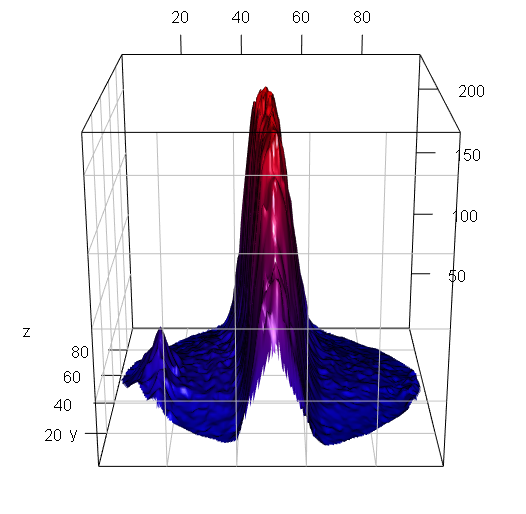
\includegraphics[scale=0.4]{bk1_2d}
        \caption{Исходные данные}
    \end{subfigure}
    \begin{subfigure}[b]{0.45\textwidth}
        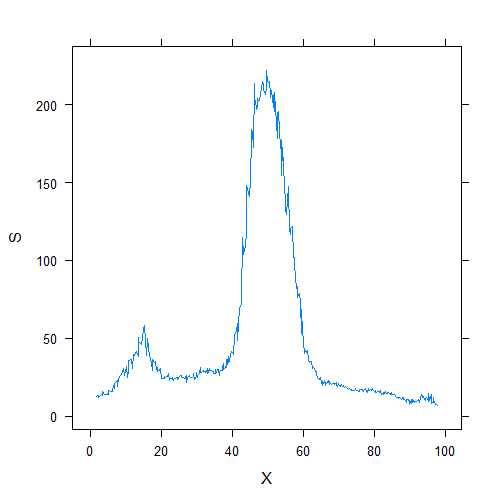
\includegraphics[scale=0.43]{bk1_1d}
        \caption{Одномерный срез}
    \end{subfigure}
    \caption{Изображение данных.}
    \label{fig:biodata}
\end{figure}  

В первом случае необходимо выделить тренд для одномерных данных, а во втором случае для двумерных.
Используем метод низких частот, задаваемый алгоритмом \ref{alg:freq1d} для одномерных данных и алгоритмом \ref{alg:freq2d} для двумерных данных.
Качество идентификации тренда можно оценивать по ошибке оценки $\sigma$.

Будем действовать следующим образом. Сначала выделим тренд для обоих случаев, беря фиксированное число компонент, затем применим алгоритмы автоматической идентификации и сравним результаты этих двух подходов.

Параметры для автоматической идентификации будем подбирать на модельных данных,
имитирующих поведение реальных. Будем использовать полученные параметры для реальных данных.
Перед 2D-SSA процедурой данные были интерполированы на регулярную решетку с шагом $\Delta = 0.5$.

В случае одномерных данных были получены значения параметров: $L=30$, $\omega=0.04$, $T_0=0.4$.
Для двумерных данных значения следующие:  $L=(10,10)$, $\omega_{1}=0.08 \Delta$,
  $\omega_{2}=0.1 \Delta$, $T_0=0.2$, где шаг интерполяции $\Delta = 0.5$.

На рис.~\ref{fig:real_data_1d} приведен график восстановленного тренда и шума на фоне исходного ряда для одномерного среза данных, 
На рис.~\ref{fig:real_data_2d} приведено изображение исходных данных, восстановленного тренда и остатка для двумерных данных. 

\begin{figure}[!hhh]
	\begin{center}
	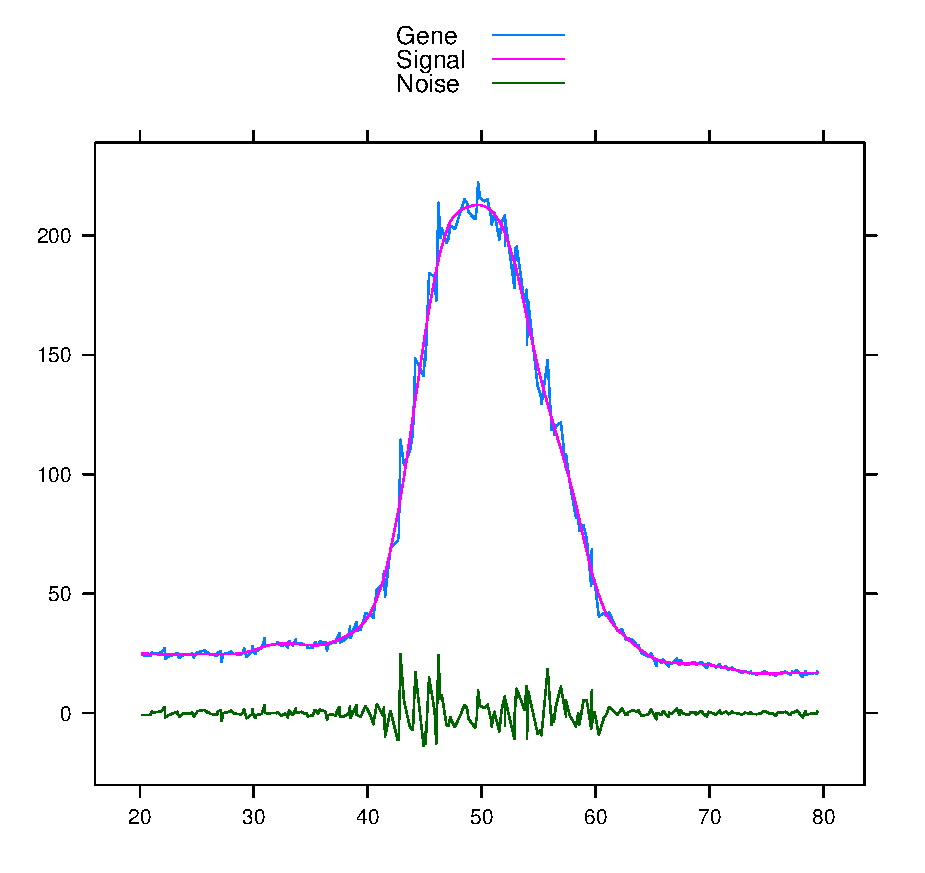
\includegraphics[scale=0.5]{real_data_trend_noise0}
	\end{center}
	\caption{Оценки тренда и шума на фоне исходных данных, одномерный срез.}
	\label{fig:real_data_1d}
\end{figure}

\begin{figure}[!hhh]
	\begin{center}
	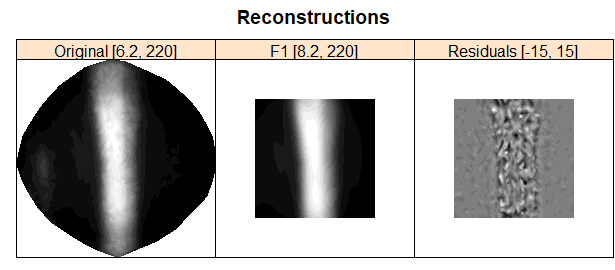
\includegraphics[scale=0.6]{bk1_2d_rec}
	\end{center}
	\caption{Изображение исходных данных, восстановленного тренда и остатка.}
	\label{fig:real_data_2d}
\end{figure}

В таблицах \ref{tab:model_est_compare} и \ref{tab:real_est_compare} представлены результаты для модельных и реальных данных гена Kruppel возраста 8.

 \begin{table}[hhh!]
\caption{Модельные данные, истинное значение параметра $\sigma^2=0.03$.}
 \centering
 \begin{tabular}{rrrrr}
  \hline
  & 1D  & 2D  & 1D auto  & 2D auto \\
  \hline
  Mean estimates & 0.0285 & 0.0311 & 0.0285 & 0.0318 \\
  sd & 0.0037 & 0.0006 & 0.0037 & 0.0008 \\
 \end{tabular}
  \label{tab:model_est_compare}
 \end{table}
  \begin{table}[hhh!]
\caption{Реальные данные, Kruppel 8.}
 \centering
 \begin{tabular}{rrrrr}
  \hline
  & 1D  & 2D   & 1D auto & 2D auto \\
  \hline
  Mean estimates & 0.0392 & 0.0347 & 0.0390 & 0.0341 \\
  sd & 0.0123 & 0.0063 & 0.0120 & 0.0054 \\
 \end{tabular}
 \label{tab:real_est_compare}
 \end{table}

Из таблиц можно сделать следующие выводы.
\begin{itemize}
\item Подход через анализ двумерных данных сработал лучше, чем подход с одномерными данными.
\item Автоматическая идентификация практически такого же качества, как идентификация с фиксированным числом компонент, т.е. автоматическая идентификация сработала верно.
\end{itemize}

\section{Приложение метода автоматической идентификации колебательной составляющей для решения задачи выделения прямых линий с зашумленного изображения}
\label{sec:use_cssa}

В данном разделе мы рассмотрим алгоритм, предложенный в \cite{Trickett2003} и также исследованный в моей бакалаврской работе \cite{Zhornikova2016}.
На одном из этапов алгоритма возникают комплексные ряды, и встает задача выделения комплексных э-м гармоник.
Для решения можно применить метод автоматической идентификации колебательной составляющей для комплексного ряда: по регулярности углов  из раздела \ref{sec:tau_cssa}, реализуемый алгоритмом \ref{alg:cssatau_2}, или частотный метод из раздела \ref{sec:freq_cssa}, реализуемый алгоритмом \ref{alg:cssa_pgram}. Продемонстрируем это.

В общих словах постановку задачи можно описать следующим образом. Пусть имеется некоторое изображение, которое пересекают прямые линии. Мы хотим выделить эти линии, т.е. получить только их изображение.
Изображение линий, которое считаем сигналом, можно воспринимать как матрицу из $0$ и $1$, а прямые линии --- как единицы, расположенные на одной прямой. Считается, что наблюдаем зашумленный сигнал, т.е. матрицу с добавленным белым шумом.
Рассматриваемый алгоритм из \cite{Trickett2003} служит для отделения сигнала от шума.

Теперь опишем формальную постановку задачи, алгоритм и приведем примеры применения.

\subsection{Задача, решаемая алгоритмом} \label{sec:chapter3_task}
Пусть $\mathbf{X}$ --- матрица изображения, которую мы наблюдаем, ее можно воспринимать как систему из $N_c$ временных рядов длины $N_t$
\begin{equation*}
	\mathbf{X}=\left\{x_{ct}=x_c(t) \; | \; c=1, \ldots, N_c, \; t=1, \ldots, N_t\right\}.
\end{equation*}

Далее, пусть $\mathbf{S}$ --- сигнал, т.е. матрица из $0$ и $1$, и все единицы матрицы образуют прямые линии, т.е. любая единица принадлежит какой-то линии, и все линии состоят только из единиц. Матрице $\mathbf{S}$ соответствует система временных рядов $s_c(t)$, $c=1, \ldots, N_c$, $t=1, \ldots, N_t$.

Считаем, что положение единиц, образующих прямую линию, задается уравнением $c = a t + b$, где $t$ --- номер столбца, а $c$ --- номер строки, в которой стоит единица, $t \in \{1,\ldots, N_t\}$, $c \in \{1,\ldots,N_c\}$.
Далее всегда предполагаем, что $a$ и $b$ заданы корректно, т.е. для ненулевого подмножества $t \in \{1,\ldots, N_t\}$ выполняется $c = a t + b \in \{1,\ldots,N_c\}$.

Например, матрица с линией из единиц, заданной уравнением $c = t + 1$, и с $N_c \geqslant N_t$ будет выглядеть так:\\
\begin{equation*}
\begin{array}{cccccccc}
   \text{строчка номер } 1: \quad & 0 & \underbrace{\bf{1}}_{2} & 0 & ... & 0 & ... & 0 \\
   \text{строчка номер } 2: \quad & 0 & 0 & \underbrace{\bf{1}}_{3} & ... & 0 & ... & 0 \\
     & ... & ... & ... & ... & ... & ... & ... \\
    \text{строчка номер } m: \quad   & 0 & 0 & 0 & ... & \underbrace{\bf{1}}_{m+1} & ... & 0  \\
       & ... & ... & ... & ... & ... & ... & ... \\
        \text{строчка номер } N_c: \quad & 0 & 0 & 0 & ... & 0 & ... & 0
   \end{array}
\end{equation*}
\\
\begin{remark}
При $a = 1$ прямая наклонена к вертикали под углом в $45$ градусов, при $a < 1 $--- под углом, большим $45$ градусов, и при $a > 1$ --- под углом, меньшим $45$ градусов.
\end{remark}

Итак, пусть мы наблюдаем матрицу
\begin{gather*}
\mathbf{X} = \mathbf{S} + \mathbf{R},
\end{gather*}
где $\mathbf{R}$ --- шум, $\mathbf{R} = \{\varepsilon_{ij}\}$, $i=1,\ldots,N_c$, $j=1,\ldots,N_t$, $\varepsilon_{ij}$ --- независимые реализации распределения $N(0,\sigma^2)$.

Задача, решаемая алгоритмом, --- по наблюдаемой матрице $\mathbf{X}$ оценить сигнал $\mathbf{S}$.

\subsection{Описание алгоритма}
\label{sec:use_cssa_algorithm}
Как уже говорилось выше, матрицу изображения $\mathbf{X}$ можно воспринимать как систему из $N_c$ временных рядов длины $N_t$
\begin{equation*}
	\mathbf{X}=\left\{x_{ct}=x_c(t) \; | \; c=1, \ldots, N_c, \; t=1, \ldots, N_t\right\}.
\end{equation*}
Т.е. исходными данными для анализа является система временных рядов.

    Весь алгоритм из \cite{Trickett2003} можно разбить на три части.
    Опишем каждый из этапов.

\begin{enumerate}
\item
{\bf Дискретное преобразование Фурье.\\}
    Вычисляем дискретное (комплексное) преобразование Фурье (сокращенно DFT)
    для каждого временного ряда исходной системы $(c=1, \ldots, N_c)$,
    и получаем матрицу $\bf\Xi$:
\begin{equation*}
\mathbf\Xi =
\left(
\begin{array}{cccc}
    \xi_1(1), & \xi_1(2), & \ldots, & \xi_1(N_t)\\
    \xi_2(1), & \xi_2(2), & \ldots, & \xi_2(N_t)\\
    \vdots & \vdots & \ddots & \vdots\\
    \xi_{N_c}(1), & \xi_{N_c}(2), & \ldots, & \xi_{N_c}(N_t)\\
\end{array}
\right),
\end{equation*}
   где
\begin{equation*}
    \xi_c(t) = \sum_{j=1}^{N_t}x_c(j)e^{-2\pi \I \frac{(j-1)(t-1)}{N_t}}.
\end{equation*}

\item
{\bf Метод CSSA.\\}
На втором этапе применяем метод CSSA
 к каждому столбцу матрицы $\bf\Xi$.
Применение метода CSSA заключается в выборе длины окна $L$ и числа компонент $M$, соответствующих сигналу,  при которых сигнал отделятся от шума.
Таким образом, восстановив по $I = \{1,\ldots,M\}$, в результате метода мы получим новую матрицу $\mathbf{\Xi}^{(1)} = \{\xi^{(1)}_c(t)\}_{t=1, c=1}^{N_t, N_c}$.

\item
{\bf Обратное преобразование Фурье.\\}
На последнем этапе применяем обратное преобразование Фурье (сокращенно IDFT)
к каждой строчке матрицы $\mathbf{\Xi}^{(1)}$.
Получаем:
\begin{gather*}
     x_c^{(1)}(t) = \frac{1}{N_c}\sum_{k=1}^{N_c}\xi_c^{(1)}(k)e^{2\pi \I \frac{(t-1)(k-1)}{N_c}},
    \quad \text{в случае IDFT по столбцам}, \\
     x_c^{(1)}(t) = \frac{1}{N_t}\sum_{k=1}^{N_t}\xi_c^{(1)}(k)e^{2\pi \I \frac{(t-1)(k-1)}{N_t}},
    \quad \text{в случае IDFT по строчкам},
\end{gather*}

Таким образом, итоговым результатом является новая матрица $\mathbf{X}^{(1)}$ или система временных рядов $x_c^{(1)}(t)$:
\begin{equation*}
    \mathbf{X}^{(1)}=\left\{x_c^{(1)}(t) \; | \; c=1, \ldots, N_c, \; t=1, \ldots, N_t\right\}.
\end{equation*}
\end{enumerate}

\subsection{Обсуждение и пример применения}
В бакалаврской работе \cite{Zhornikova2016} было доказано следующее утверждение о том, что описанный алгоритм из предыдущего раздела можно применять для выделения нескольких линий.

\begin{Th} \cite[Утверждение 20]{Zhornikova2016}
Пусть матрица $\mathbf{X}$ состоит только из $0$ и $1$ и все единицы стоят на $m$ прямых, задаваемых уравнениями $c = a_i\,t + b_i$,  $a_i \leqslant 1$ и $N_c \leqslant a_i\,N_t + b_i$, $i=1,\ldots,m$. Пусть также для любого $i$
область значений $c = a_i t + b_i$ равняется $\{1,\ldots,N_c\}$.
Применим к матрице алгоритм из раздела \ref{sec:use_cssa_algorithm}, на этапе CSSA используем $M = m$ и $m<L<N$. Тогда результат работы алгоритма будет равен исходной матрице $\mathbf{X}$.
\end{Th}

Таким образом, на этапе CSSA мы можем применить алгоритм \ref{alg:cssatau_2} метода выделения комплексных э-м гармоник из раздела \ref{sec:tau_cssa} для случая, когда количество э-м гармоник известно с $m$, равным количеству линий. Алгоритм \ref{alg:cssa_pgram} также, как и алгоритм \ref{alg:cssatau_2} можно обобщить на случай, когда число э-м гармоник, которые хотим выделить, известно. Просто сортируем значения $\rho_i$ из формулы \eqref{eq:rho_i_cssa} по убыванию и берем первые $m$ компонент. 

Перейдем к самому примеру.
Возьмем $N_t = 120$, $N_c = 100$, $\sigma = 0.2$ и рассмотрим изображение с двумя прямыми, задаваемыми уравнениями $c = t + 3$ и $c = 110 - t$ соответственно. Тогда на вход мы получаем матрицу, изображенную на рис.~\ref{fig:a_many_before}.

На рис.~\ref{fig:a_many_after} изображен результат применения алгоритма без автоматической группировки на этапе CSSA, когда просто восстанавливаем по первым двум компонентам. На рис.~\ref{fig:a_many_after2} изображен результат с применением алгоритма \ref{alg:cssatau_2} метода по регулярности углов с $m=2$. 
Результат применения с модернизированным (для случая, когда число э-м гармоник известно) частотным алгоритмом (используем значение $s_0 = 1$) представлен на рис.~\ref{fig:a_many_after3}.
Видим, что все три варианта значительно очистили изображение от шума, но частотный метод сработал немного хуже, чем два других варианта.
\begin{figure}
        \centering
      \begin{subfigure}[b]{0.45\textwidth}
        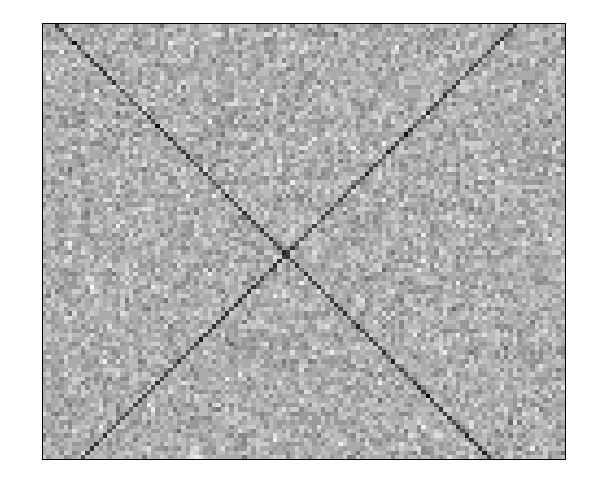
\includegraphics[width=\textwidth]{lines_noise}
        \caption{До алгоритма.}
        \label{fig:a_many_before}
    \end{subfigure}
        \quad       
  \begin{subfigure}[b]{0.45\textwidth}
      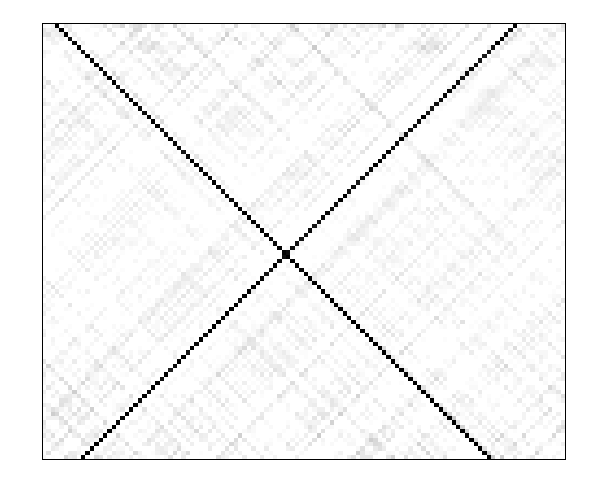
\includegraphics[width=\textwidth]{noauto_lines}
        \caption{После, без АИ.}
        \label{fig:a_many_after}
    \end{subfigure}
    \begin{subfigure}[b]{0.45\textwidth}
        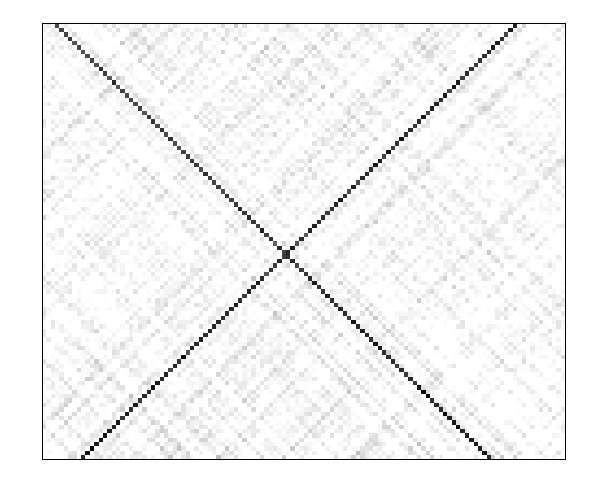
\includegraphics[width=\textwidth]{auto_lines}
        \caption{После, с АИ, алгоритм \ref{alg:cssatau_2}.}
        \label{fig:a_many_after2}
    \end{subfigure}
        \quad
        \begin{subfigure}[b]{0.45\textwidth}
       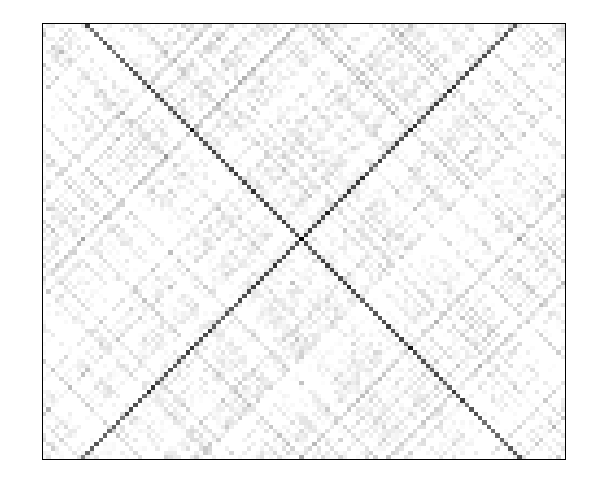
\includegraphics[width=\textwidth]{auto_lines_freq}
        \caption{После, с АИ, алгоритм \ref{alg:cssa_pgram}.}
        \label{fig:a_many_after3}
    \end{subfigure}
       \caption{Изображение с двумя линиями.}\label{fig:a_many}
\end{figure}

\chapter{Реализация методов автоматической идентификации в R}
\label{sec:code}
\section{Описание функций}

Реализация алгоритма SSA для всех методов 1D-SSA, CSSA, MSSA, 2D-SSA есть в R-пакетe \textsc{Rssa} \cite{Rssa, Golyandina.Korobeynikov2013}. Для применения нужно воспользоваться функциями ssa для разложения и reconstruct для восстановления.
У ssa есть параметр kind, который может принимать значения <<1d-ssa>>, <<mssa>>, <<cssa>>, <<2d-ssa>>; у reconstruct есть параметр groups, в котором можно задать группы, по которым хотим восстановить составляющие. 

Алгоритм \ref{alg:wcor} кластерного метода группировки и алгоритм \ref{alg:freq1d} метода низких частот для идентификации тренда для 1D-SSA  реализованы в R-пакетe \textsc{Rssa}.
Используется функция grouping.auto, у которой есть параметр grouping.method. Параметр принимает два значения, соответствующие разным методам: <<wcor>> --- алгоритм \ref{alg:wcor} кластерного метода группировки и  <<pgram>> --- алгоритм \ref{alg:freq1d} метода низких частот. 

Многие другие алгоритмы были реализованы мной в рамках данной работы: алгоритм \ref{alg:1d_pgram} частотного метода идентификации для 1D-SSA, алгоритм \ref{alg:1dtau_2} метода по регулярности углов для 1D-SSA и все алгоритмы из главы \ref{sec:all_methods} кроме кластерного метода группировки. Код реализаций можно найти по ссылке \cite{polina_zhornikova_2018_1252476}. Далее будет приведено описание этих реализаций.


Имеется главная функция general.grouping.auto, имеющая параметр grouping.method, который может принимать следующие значения. 
\begin{enumerate}
\item <<low.freq.cssa>> --- метод низких частот идентификации тренда для CSSA, реализуемый алгоритмом \ref{alg:freqcssa}. Метод имеет параметры:
\begin{itemize}
\item freq.bins --- частота $\omega$, по умолчанию freq.bins = 0.01;
\item theshold --- порог $T_0$, по умолчанию theshold = 0.9.
\end{itemize}
\item <<low.freq.cssa>> --- метод низких частот идентификации тренда для CSSA, реализуемый алгоритмами \ref{alg:freqmssa_1}, \ref{alg:freqmssa_2}. Метод имеет параметры:
\begin{itemize}
\item base, принимающий одно из трех значений <<series>>, <<eigen>>, <<factor>>, означающее, что метод применяется либо к элементарным восстановленным рядам, либо к левым сингулярным векторам, либо к правым сингулярным векторам соответственно;
\item freq.bins --- частота $\omega$, по умолчанию freq.bins = 0.01;
\item theshold --- порог $T_0$, по умолчанию theshold = 0.9.
\end{itemize} 
\item <<low.freq.2dssa>> --- метод низких частот идентификации тренда для 2D-SSA, реализуемый алгоритмом \ref{alg:freq2d}. Метод имеет параметры:
\begin{itemize}
\item base, принимающий одно из трех значений <<series>>, <<eigen>>, <<factor>>, означающее, что метод применяется либо к восстановленным полям, либо к левым сингулярным векторам, либо к правым сингулярным векторам соответственно;
\item freq.bins1 --- частота $\omega_1$, freq.bins2 --- частота $\omega_2$; по умолчанию freq.bins1 = freq.bins2 = 0.1;
\item theshold --- порог $T_0$, по умолчанию theshold = 0.8.
\end{itemize} 
\item <<freq.1dssa>> --- частотный метод идентификации колебательной составляющей для 1D-SSA, реализуемый алгоритмом \ref{alg:1d_pgram}. Метод имеет параметры:
\begin{itemize}
\item s\_0 --- параметр $s_0$, по умолчанию s\_0=1;
\item rho\_0 --- порог $\rho_0$, по умолчанию rho\_0= 0.9.
\end{itemize} 
\item <<freq.cssa>> --- частотный метод идентификации колебательной составляющей для 1D-SSA, реализуемый алгоритмом \ref{alg:cssa_pgram}. Метод имеет параметры:
\begin{itemize}
\item s\_0 --- параметр $s_0$, по умолчанию s\_0=1;
\item rho\_0 --- порог $\rho_0$, по умолчанию rho\_0= 0.9.
\end{itemize} 
\item <<freq.mssa>> --- частотный метод идентификации колебательной составляющей для 1D-SSA, реализуемый алгоритмами \ref{alg:mssa_pgram_1}, \ref{alg:mssa_pgram_2}. Метод имеет параметры:
\begin{itemize}
\item base, принимающий одно из двух значений  <<eigen>>, <<factor>>, означающее, что метод применяется либо к  к левым сингулярным векторам, либо к правым сингулярным векторам соответственно;
\item s\_0 --- параметр $s_0$, по умолчанию s\_0=1;
\item rho\_0 --- порог $\rho_0$, по умолчанию rho\_0= 0.9.
\end{itemize} 
\item <<tau.1dssa>> --- метод идентификации колебательной составляющей по регулярности углов для 1D-SSA, реализуемый алгоритмом \ref{alg:1dtau_2}. Метод имеет параметры:
\begin{itemize}
\item threshold --- порог $t_0$, по умолчанию $t_0=0.01$;
\item numcomp --- количество составляющих, которые хотим идентифицировать, если numcomp = 0, то применяется вариант с использованием порога; по умолчанию numcomp = 0.
\end{itemize} 
\item <<tau.сssa>> --- метод идентификации колебательной составляющей по регулярности углов для CSSA, реализуемый алгоритмом \ref{alg:1dtau_2}. Метод имеет параметры:
\begin{itemize}
\item threshold --- порог $t_0$, по умолчанию $t_0=0.01$;
\item numcomp1 --- количество э-м гармоник ранга 1, которые хотим идентифицировать, numcomp2 --- количество э-м гармоник ранга 2, которые хотим идентифицировать; если numcomp1 = 0, то для $d=1$ применяется вариант с использованием порога, и аналогично для numcomp2; по умолчанию numcomp1 = 0 и numcomp2 = 0.
\end{itemize} 
\item <<tau.mssa>> --- метод идентификации колебательной составляющей по регулярности углов для MSSA, реализуемый алгоритмом \ref{alg:tau_mssa}. Метод имеет параметры:
\begin{itemize}
\item base, принимающий одно из двух значений  <<eigen>>, <<factor>>, означающее, что метод применяется либо к  к левым сингулярным векторам, либо к правым сингулярным векторам соответственно;
\item threshold --- порог $t_0$, по умолчанию $t_0=0.01$;
\item numcomp --- количество составляющих, которые хотим идентифицировать, если numcomp = 0, то применяется вариант с использованием порога; по умолчанию numcomp = 0.
\end{itemize} 
\end{enumerate}

\section{Примеры применений}
Приведем примеры кода и результатов работы всех алгоритмов на простых модельных примерах.

\subsection{1D-SSA}
Для начала рассмотрим 1D-SSA и вещественный одномерный ряд.

Во фрагменте \ref{frag:1dssa_init} подключаем файл с функцией автоматической идентификации, пакет lattice для графиков и пакет Rssa для применения SSA, задаем основные параметры для ряда: N (длина ряда), omega1 и omega2 (частоты для э-м гармоник).
\begin{fragment}[1D-SSA: инициализация]
\label{frag:1dssa_init}
\begin{CodeChunk}
\begin{CodeInput}


> source('main.grouping.auto.R')
> library(lattice)
> library(Rssa)
> N <- 199
> omega1 <- 0.1
> omega2 <- 0.3
\end{CodeInput}

\end{CodeChunk}
\end{fragment}
Во фрагменте \ref{frag:1dssa_series} задаем ряд x, который состоит из тренда, задаваемого экспонентой с показателем 0.01, гармоники с частотой omega1, э-м гармоники с частотой omega2 и показателем экспоненты 0.009, гармоники с периодом 0.5 и нормального белого шума с нулевым средним и дисперсией 1.
Дальше применяем SSA с длиной окна $L=100$.
\begin{fragment}[1D-SSA: задание ряда и применение SSA]
\label{frag:1dssa_series}
\begin{CodeChunk}
\begin{CodeInput}


> x <- exp(0.01 * (1:N)) + 2*cos(2 * pi * omega1 * (1:N)) +  
+   exp(0.009 * (1:N)) * cos(2 * pi * omega2 * (1:N)) + 
+   2*cos(2 * pi * 0.5 * (1:N))+ rnorm(N,1.5)
> s <- ssa(x, L = 100)
> plot(s, type="vectors", layout = c(5, 2))
> plot(s, type="paired", layout = c(5, 2))
\end{CodeInput}

\end{CodeChunk}
\end{fragment}
На рис.~\ref{fig:1dssa_vectors} приведен вид левых сингулярных векторов для ряда x. Видно, что первый вектор относится к тренду; второй вектор к гармонике ранга 1; пары 3--4 и 5--6 к гармоникам ранга 2. Последнее также подтверждает рис.~\ref{fig:1dssa_vectors_pair}, на котором изображены двумерные диаграммы сингулярных векторов.
\bfgh
        \begin{center}
{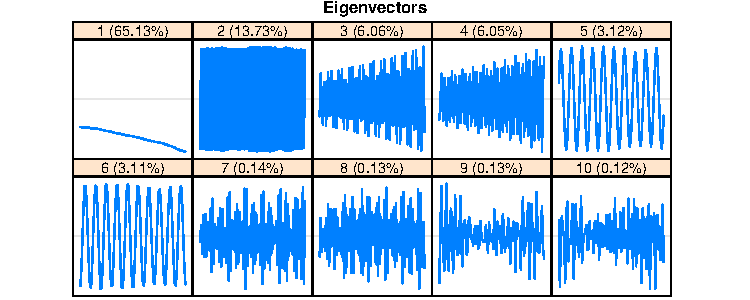
\includegraphics[width=4.5in]{1dssa_vectors}}
        \end{center}
        \caption{1D-SSA пример. Левые сингулярные вектора}
        \label{fig:1dssa_vectors}
\efg
\bfgh
        \begin{center}
{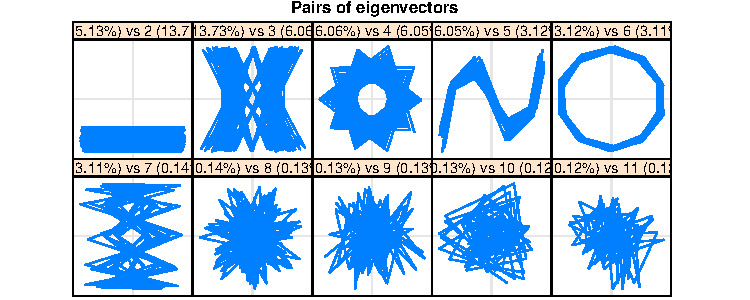
\includegraphics[width=4.5in]{1dssa_vectors_pair}}
        \end{center}
        \caption{1D-SSA пример. Двумерные диаграммы левых сингулярных векторов}
        \label{fig:1dssa_vectors_pair}
\efg

Теперь перейдем к применению методов автоматической группировки, во фрагменте \ref{frag:1dssa_trend} применяем метод низких частот для тренда из пакета Rssa с помощью функции grouping.auto. Используем значение 0.01 для частоты и 0.9 для порога, функция выделила только одну первую компоненту. 
\begin{fragment}[1D-SSA пример. Идентификация тренда, алгоритм \ref{alg:freq1d}]
\label{frag:1dssa_trend}
\begin{CodeChunk}
\begin{CodeInput}


> g_trend <- grouping.auto(s, grouping.method = 'pgram',
+   freq.bins = list(0.01), threshold = 0.9)
> print(g_trend$F1)
[1] 1
\end{CodeInput}

\end{CodeChunk}
\end{fragment}
Далее во фрагменте \ref{frag:1dssa_em_freq}, используя созданную функцию general.grouping.auto, применим частотный метод идентификации колебательной составляющей. Используем значения $s_0 = 1$, $\rho_0 = 0.9$. 
Метод выдает две группы индексов: I\_1 --- индексы компонент с частотой $\omega \not = 0.5$, и I\_2 --- индексы компонент с частотой $\omega = 0.5$.
Видим, что метод выделим все нужные компоненты 2--6.
\begin{fragment}[1D-SSA пример. Идентификация э-м гармоник,  алгоритм \ref{alg:1d_pgram}]
\label{frag:1dssa_em_freq}
\begin{CodeChunk}
\begin{CodeInput}


> g_em_freq <- general.grouping.auto(s, grouping.method = "freq.1dssa", s_0 = 1, 
+                                  rho_0 = 0.9)
> print(g_em_freq)
$I_1
[1] 3 4 5 6
$I_2
[1] 2
\end{CodeInput}

\end{CodeChunk}
\end{fragment}
Во фрагменте \ref{frag:1dssa_em_tau} применяем метод идентификации колебательной составляющей по регулярности углов, используем $t_0 = 0.01$. Метод выделил компоненты 3-6, относящиеся к э-м гаромникам ранга 2. Гармонику с частотой 0.5, как уже отмечалось в разделе \ref{sec:tau1}, метод выделять не умеет, поэтому компоненту 2 метод не выделил. 
\begin{fragment}[1D-SSA пример. Идентификация э-м гармоник, алгоритм \ref{alg:1dtau_2}]
\label{frag:1dssa_em_tau}
\begin{CodeChunk}
\begin{CodeInput}


> g_em_tau <- general.grouping.auto(s, grouping.method = "tau.1dssa", treshold = 0.01)
> print(g_em_tau$idx)
[1] 3 4 5 6
\end{CodeInput}

\end{CodeChunk}
\end{fragment}
Теперь во фрагменте \ref{frag:1dssa_rec} восстановим тренд и колебательную составляющую с помощью полученных групп g\_trend, g\_em\_freq и функции reconstruct из пакета Rssa, на рис.~\ref{fig:1dssa_rec} приведен график восстановленных компонент на фоне исходного ряда.
\begin{fragment}[1D-SSA пример. Восстановление составляющих]
\label{frag:1dssa_rec}
\begin{CodeChunk}
\begin{CodeInput}


> r <- reconstruct(s, groups = list(T = g_trend, P = c(g_em_freq$I_1, 
+                                                      g_em_freq$I_2)))
> d <- data.frame(X=x, N=1:N, T=r$T, P=r$P)
> xyplot(T + P +X ~ N, data = d, type ='l', ylab = '',
+        auto.key = list(points = FALSE, lines = TRUE))
\end{CodeInput}

\end{CodeChunk}
\end{fragment}
\bfgh
        \begin{center}
{\includegraphics[width=4.5in]{1dssa_rec}}
        \end{center}
        \caption{1D-SSA пример. Восстановленные компоненты на фоне исходного ряда}
        \label{fig:1dssa_rec}
\efg


\subsection{CSSA}
В случае с CSSA используется тот же фрагмент \ref{frag:1dssa_init} для инициализации.

Во фрагменте \ref{frag:cssa_series} задаем комплексный ряд x, который состоит из тренда, задаваемого экспонентой с показателем 0.01, комплексной гармоники ранга 1 с частотой omega1, комплексной э-м гармоники с частотой omega2 и показателем экспоненты 0.007 и нормального белого шума с нулевым средним и дисперсией 1.
Дальше применяем SSA с длиной окна $L=100$.
\begin{fragment}[CSSA пример. Задание ряда и применение SSA]
\label{frag:cssa_series}
\begin{CodeChunk}
\begin{CodeInput}


> x <- exp(0.01 * (1:N)) + cos(2 * pi * omega1 * (1:N)) + 
+   1.0i*sin(2 * pi * omega1 * (1:N)) + 
+   1.0i*exp(0.007 * (1:N))*cos(2 * pi * omega2 * (1:N)) + rnorm(N, 1) 
> s <- ssa(x, kind = 'cssa', L = 100)
> plot(s, type="vectors", layout = c(5, 2))
\end{CodeInput}

\end{CodeChunk}
\end{fragment}
На рис.~\ref{fig:cssa_vectors} приведен вид левых сингулярных векторов для ряда x. Похоже, что первый вектор относится к тренду; пара векторов 2 и 4 к гармонике ранга 2 и вектор 3 к гармонике ранга 1.
\bfgh
        \begin{center}
{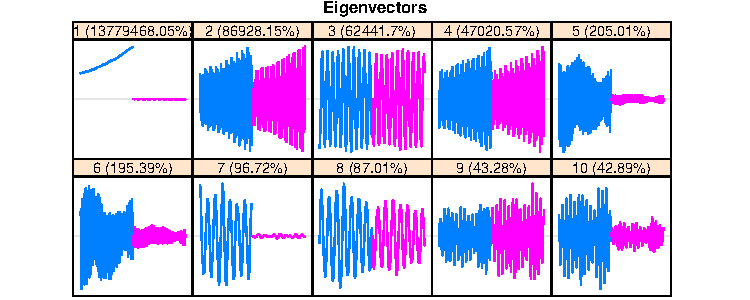
\includegraphics[width=4.5in]{cssa_vectors}}
        \end{center}
        \caption{CSSA пример. Левые сингулярные вектора}
        \label{fig:cssa_vectors}
\efg

Применим методы автоматической группировки, во фрагменте \ref{frag:cssa_trend} применяем метод низких частот для тренда, используя созданную функцию general.grouping.auto. Используем значение 0.01 для частоты, 0.9 для порога и элементарные восстановленные ряды (значение по умолчанию). Функция выделила только одну первую компоненту. 
\begin{fragment}[CSSA пример. Идентификация тренда, алгоритм \ref{alg:freqcssa}]
\label{frag:cssa_trend}
\begin{CodeChunk}
\begin{CodeInput}


> g_trend <- general.grouping.auto(s, grouping.method = 'low.freq.cssa', 
+                                freq.bins = list(0.01), threshold = 0.9)
> print(g_trend$F1)
[1] 1
\end{CodeInput}

\end{CodeChunk}
\end{fragment}
Далее во фрагменте \ref{frag:cssa_em_freq} применим частотный метод идентификации колебательной составляющей, используем значения $s_0 = 1$, $\rho_0 = 0.95$. Видим, что метод выделил все нужные компоненты со 2 по 4.
\begin{fragment}[CSSA пример. Идентификация э-м гармоник,  алгоритм \ref{alg:cssa_pgram}]
\label{frag:cssa_em_freq}
\begin{CodeChunk}
\begin{CodeInput}


> g_em_freq <- draft.grouping.auto(s, grouping.method = "freq.cssa", s_0 = 1, 
+                                  rho_0 = 0.95)
> print(g_em_freq)
[1] 2 3 4
\end{CodeInput}

\end{CodeChunk}
\end{fragment}

Во фрагменте \ref{frag:cssa_series} применяем метод идентификации колебательной составляющей по регулярности углов, используем $t_0 = 0.01$. Метод выдает вместе индексы и для $d=1$, и для $d=2$. 
Видим, что метод выделил все компоненты 2--4, относящиеся к э-м гармоникам.

\begin{fragment}[CSSA пример. Идентификация э-м гармоник, алгоритм \ref{alg:cssatau_2}]
\label{frag:cssa_em_tau}
\begin{CodeChunk}
\begin{CodeInput}


> g_em_tau <- general.grouping.auto(s, grouping.method = "tau.cssa", treshold = 0.01)
> print(g_em_tau$idx)
[1] 2 3 4
\end{CodeInput}

\end{CodeChunk}
\end{fragment}

Во фрагменте \ref{frag:cssa_rec} восстановим тренд и колебательную составляющую с помощью полученных групп g\_trend, g\_em\_tau и функции reconstruct из пакета Rssa, на рис.~\ref{fig:cssa_rec} приведен график вещественных частей восстановленных компонент на фоне вещественной части исходного ряда.
\begin{fragment}[CSSA пример. Восстановление составляющих]
\label{frag:cssa_rec}
\begin{CodeChunk}
\begin{CodeInput}


> r <- reconstruct(s, groups = list(T = g_trend, P = g_em_tau$idx))
> d_re <- data.frame(T_re = Re(r$T), P_re = Re(r$P),  X_re = Re(x), N = 1:N)
> xyplot(T_re + P_re + X_re  ~ N, data = d_re, type ='l', ylab = '',
+        auto.key = list(points = FALSE, lines = TRUE))
\end{CodeInput}

\end{CodeChunk}
\end{fragment}
\bfgh
        \begin{center}
{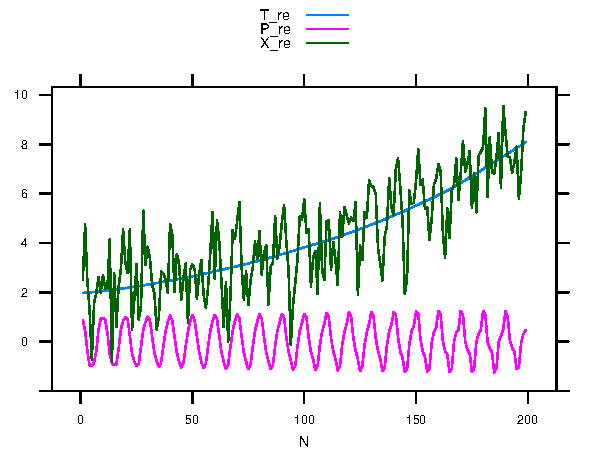
\includegraphics[width=4.5in]{cssa_rec}}
        \end{center}
        \caption{CSSA пример. Восстановленные компоненты на фоне исходного ряда}
        \label{fig:cssa_rec}
\efg



\subsection{MSSA}
Рассмотрим пример с двумя рядами. Во фрагменте \ref{frag:mssa_init} подключаем файл с функцией автоматической идентификации, пакет lattice для графиков и пакет Rssa для применения SSA, задаем основные параметры для системы рядов: N.A, N.B (длины рядов), omega1 (частота для э-м гармоник).
\begin{fragment}[MSSA: инициализация]
\label{frag:mssa_init}
\begin{CodeChunk}
\begin{CodeInput}


> source('main.grouping.auto.R')
> library(lattice)
> library(Rssa)
> N.A <- 150
> N.B <- 120
> omega1 <- 0.1
\end{CodeInput}

\end{CodeChunk}
\end{fragment}
Во фрагменте \ref{frag:mssa_series} задаем многомерный ряд X, который состоит из тренда, задаваемого экспонентой с показателем 0.01, гармоники с частотой omega1, гаромники ранга 1 с частотой 0.5 и нормального белого шума с нулевым средним и дисперсией 1. Все компоненты кроме тренда присутствуют в обоих рядах (обозначаемых в коде, как A и B), тренд присутствует только в компоненте A.
Дальше применяем SSA с длиной окна $L=60$.
\begin{fragment}[MSSA пример. Задание ряда и применение SSA]
\label{frag:mssa_series}
\begin{CodeChunk}
\begin{CodeInput}


> tt.A <- 1:N.A
> tt.B <- 1:N.B
> X1 <- list(A = 2 * sin(2*pi * omega1 * tt.A), B = cos(2*pi * omega1 * tt.B))
> X2 <- list(A = sin(2*pi * 0.5 * tt.A), B = cos(2*pi * 0.5 * tt.B))
> X3 <- list(A = exp(0.01 * tt.A))
> X4 <- list(A=rnorm(tt.A, 1), B=rnorm(tt.B, 1))
> X <- list(A = X1$A + X2$A + X3$A+ X4$A, B = X1$B + X2$B + X4$B)
> s <- ssa(X, kind = "mssa")
> plot(s,type='vectors')
\end{CodeInput}

\end{CodeChunk}
\end{fragment}
На рис.~\ref{fig:mssa_vectors} приведен вид левых сингулярных векторов для ряда X. Похоже, что первый вектор относится к тренду; пара векторов 2-3 к гармонике ранга 2 и вектор 4 к гармонике ранга 1.
\bfgh
        \begin{center}
{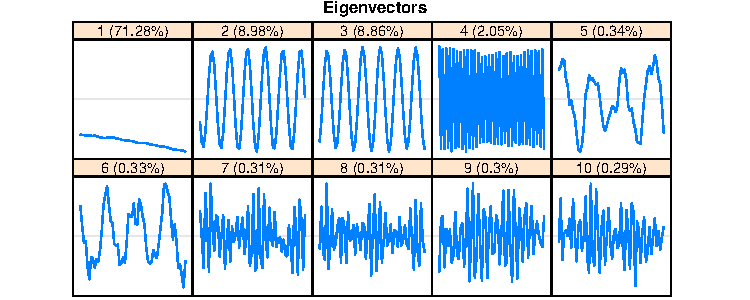
\includegraphics[width=4.5in]{mssa_vectors}}
        \end{center}
        \caption{MSSA пример. Левые сингулярные вектора}
        \label{fig:mssa_vectors}
\efg

Теперь перейдем к применению методов автоматической группировки, во фрагменте \ref{frag:mssa_trend} применяем метод низких частот для тренда, используя созданную функцию general.grouping.auto. Используем значение 0.01 для частоты и 0.9 для порога и, просто для примера, правые сингулярные вектора (т.е. base="factor"), функция выделила только одну первую компоненту. 
\begin{fragment}[MSSA пример. Идентификация тренда, алгоритм \ref{alg:freqmssa_2}]
\label{frag:mssa_trend}
\begin{CodeChunk}
\begin{CodeInput}


> g_trend <- general.grouping.auto(s, grouping.method = 'low.freq.mssa', 
+                                base='factor',
+                                freq.bins = list(0.01), threshold = 0.9)
> print(g_trend$F1)
[1] 1
\end{CodeInput}

\end{CodeChunk}
\end{fragment}
Далее во фрагменте \ref{frag:mssa_em_freq} применим частотный метод идентификации колебательной составляющей, используем значения $s_0 = 1$, $\rho_0 = 0.95$ и правые сингулярные вектора (т.е. base="factor"). Видим, что метод выделил все нужные компоненты 2-4.
\begin{fragment}[MSSA пример. Идентификация э-м гармоник,  алгоритм \ref{alg:mssa_pgram_2}]
\label{frag:mssa_em_freq}
\begin{CodeChunk}
\begin{CodeInput}


> g_em_freq <- draft.grouping.auto(s, grouping.method = "freq.mssa", base='factor',
+                                  s_0 = 1, rho_0 = 0.9)
> print(g_em_freq)
$I_1
[1] 2 3
$I_2
[1] 4
\end{CodeInput}

\end{CodeChunk}
\end{fragment}
Во фрагменте \ref{frag:mssa_em_tau} применяем метод идентификации колебательной составляющей по регулярности углов, используем $t_0 = 0.01$ и левые сингулярные вектора (т.е. base="eigen", значение по умолчанию).  Видим, что метод выделил компоненты 2-3, относящиеся к гармонике ранга 2, а компоненту 4 метод не выделил, потому что не умеет выделять компоненты с частотой 0.5.
\begin{fragment}[MSSA пример. Идентификация э-м гармоник, алгоритм \ref{alg:tau_mssa}]
\label{frag:mssa_em_tau}
\begin{CodeChunk}
\begin{CodeInput}


> g_em_tau <- draft.grouping.auto(s, grouping.method = "tau.mssa", treshold = 0.02)
> print(g_em_tau$idx)
[1] 2 3
\end{CodeInput}

\end{CodeChunk}
\end{fragment}
Теперь во фрагменте \ref{frag:mssa_rec} восстановим тренд и колебательную составляющую с помощью полученных групп g\_trend, g\_em\_tau и функции reconstruct из пакета Rssa, на рис.~\ref{fig:mssa_rec} приведен график восстановленных компонент для ряда A на фоне исходного ряда A.
\begin{fragment}[CSSA пример. Восстановление составляющих]
\label{frag:mssa_rec}
\begin{CodeChunk}
\begin{CodeInput}


> r <- reconstruct(s, groups = list(T = g_trend$F1, P = g_em_tau$idx))
> d_A <- data.frame(T_A = r$T$A, P_A = r$P$A,  X_A = X$A, N = 1:N.A)
> xyplot(T_A + P_A + X_A  ~ N, data = d_A, type ='l', ylab = '',
+        auto.key = list(points = FALSE, lines = TRUE))
\end{CodeInput}

\end{CodeChunk}
\end{fragment}
\bfgh
        \begin{center}
{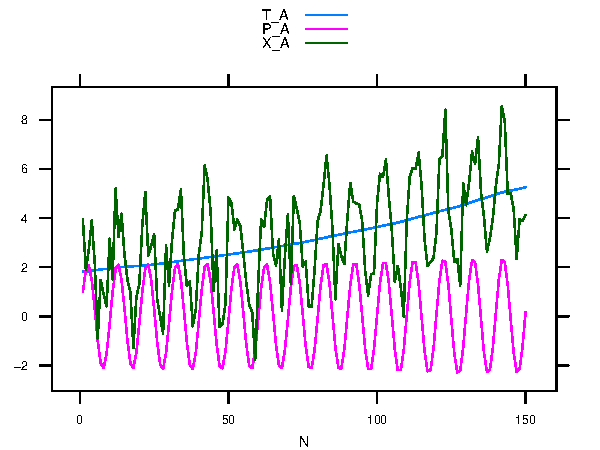
\includegraphics[width=4.5in]{mssa_rec}}
        \end{center}
        \caption{MSSA пример. Восстановленные компоненты на фоне исходного ряда}
        \label{fig:mssa_rec}
\efg


\subsection{2D-SSA}
Рассмотрим пример с 2D-SSA и двумерным изображением. Во фрагменте \ref{frag:2dssa_init} подключаем файл с функцией автоматической идентификации, пакет lattice для графиков и пакет Rssa для применения SSA, задаем основные параметры для изображения: N\_x --- ширина, N\_y --- длина; omega1 (частота для косинуса).
\begin{fragment}[2D-SSA: инициализация]
\label{frag:2dssa_init}
\begin{CodeChunk}
\begin{CodeInput}


> source('main.grouping.auto.R')
> library(lattice)
> library(Rssa)
> N_x <- 99
> N_y <- 149
> omega1 <- 0.1
\end{CodeInput}

\end{CodeChunk}
\end{fragment}
Во фрагменте \ref{frag:2dssa_series} задаем изображение matr, которое состоит из тренда, задаваемого экспонентой с показателем 0.01, косинуса с частотой omega1 и
 нормального белого шума с нулевым средним и дисперсией 0.25. 
Дальше применяем SSA с длиной окна $(L_x, L_y)=(50,50)$.
\begin{fragment}[2D-SSA пример. Задание ряда и применение SSA]
\label{frag:2dssa_series}
\begin{CodeChunk}
\begin{CodeInput}


> matr <- matrix(1,N_x,N_y)
> for (i in (1:N_x)){
+   for (j in (1:N_y)){
+     matr[i,j] <- exp(0.01 * i) + cos(2 * pi * omega1 * (i + j))  + 
+       rnorm(1,sd=0.5)
+   }
+ }
> plot2d(matr)
> s <- ssa(matr, kind = "2d-ssa", L = c(50, 50))
> plot(s, type = "vectors", cuts = 255, layout = c(4, 2))
\end{CodeInput}

\end{CodeChunk}
\end{fragment}
На рис.~\ref{fig:2dssa_series} приведено получившиеся изображение; plot2d --- специально созданная функция, код которой можно найти в \cite{polina_zhornikova_2018_1252476}.

На рис.~\ref{fig:2dssa_vectors} приведен вид левых сингулярных векторов для ряда X, сведенных к матрице способом, как было описано в разделе \ref{sec:freq_method_2d}. Похоже, что первая компонента относится к тренду, а 2-3 к гармонике.
\bfgh
        \begin{center}
{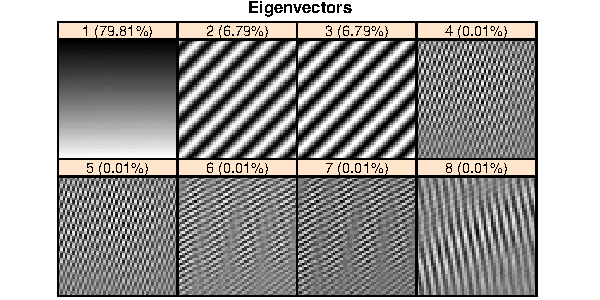
\includegraphics[width=4.5in]{2dssa_vectors}}
        \end{center}
        \caption{2D-SSA пример. Левые сингулярные вектора}
        \label{fig:2dssa_vectors}
\efg

Применим методы автоматической группировки, во фрагменте \ref{frag:2dssa_trend} применяем метод низких частот для тренда, используя созданную функцию general.grouping.auto. Используем значения $\omega_1 = \omega_2= 0.1$  для частот и 0.7 для порога $T_0$ и элементарные восстановленные поля (т.е. base="series"), функция выделила первую компоненту. 
\begin{fragment}[2D-SSA пример. Идентификация тренда, алгоритм \ref{alg:freq2d}]
\label{frag:2dssa_trend}
\begin{CodeChunk}
\begin{CodeInput}


> g_trend <- draft.grouping.auto(s, grouping.method="low.freq.2dssa", 
+                                freq.bins1 = 0.1, freq.bins2 = 0.1,
+                                threshold = 0.7, base='series')
> print(g_trend$g)
[1] 1
\end{CodeInput}

\end{CodeChunk}
\end{fragment}

Во фрагменте \ref{frag:2dssa_rec} восстановим тренд с помощью полученной группы g\_trend и  функции reconstruct из пакета Rssa, на рис.~\ref{fig:2dssa_rec} приведено изображение восстановленного тренда.
\begin{fragment}[2D-SSA пример. Восстановление составляющих]
\label{frag:2dssa_rec}
\begin{CodeChunk}
\begin{CodeInput}


> r <- reconstruct(s, groups = list(T = g_trend$g))
> plot2d(r$T)
\end{CodeInput}

\end{CodeChunk}
\end{fragment}
\begin{figure}[hhh!]
        \centering
    \begin{subfigure}[b]{0.45\textwidth}
        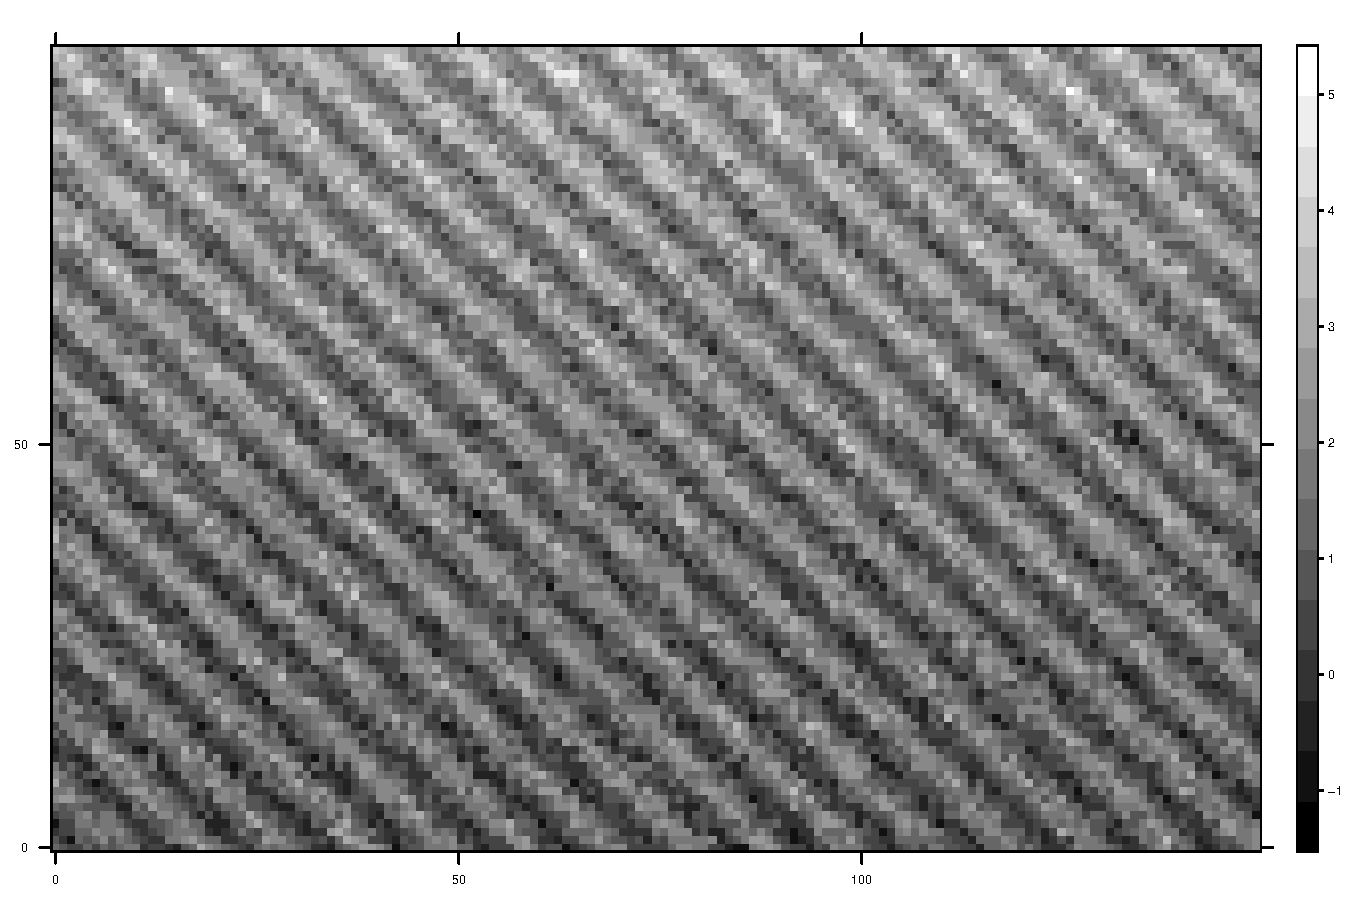
\includegraphics[width=\textwidth]{2dssa_series}
        \caption{Исходное изображение.}
        \label{fig:2dssa_series}
    \end{subfigure}
        \quad
    \begin{subfigure}[b]{0.45\textwidth}
       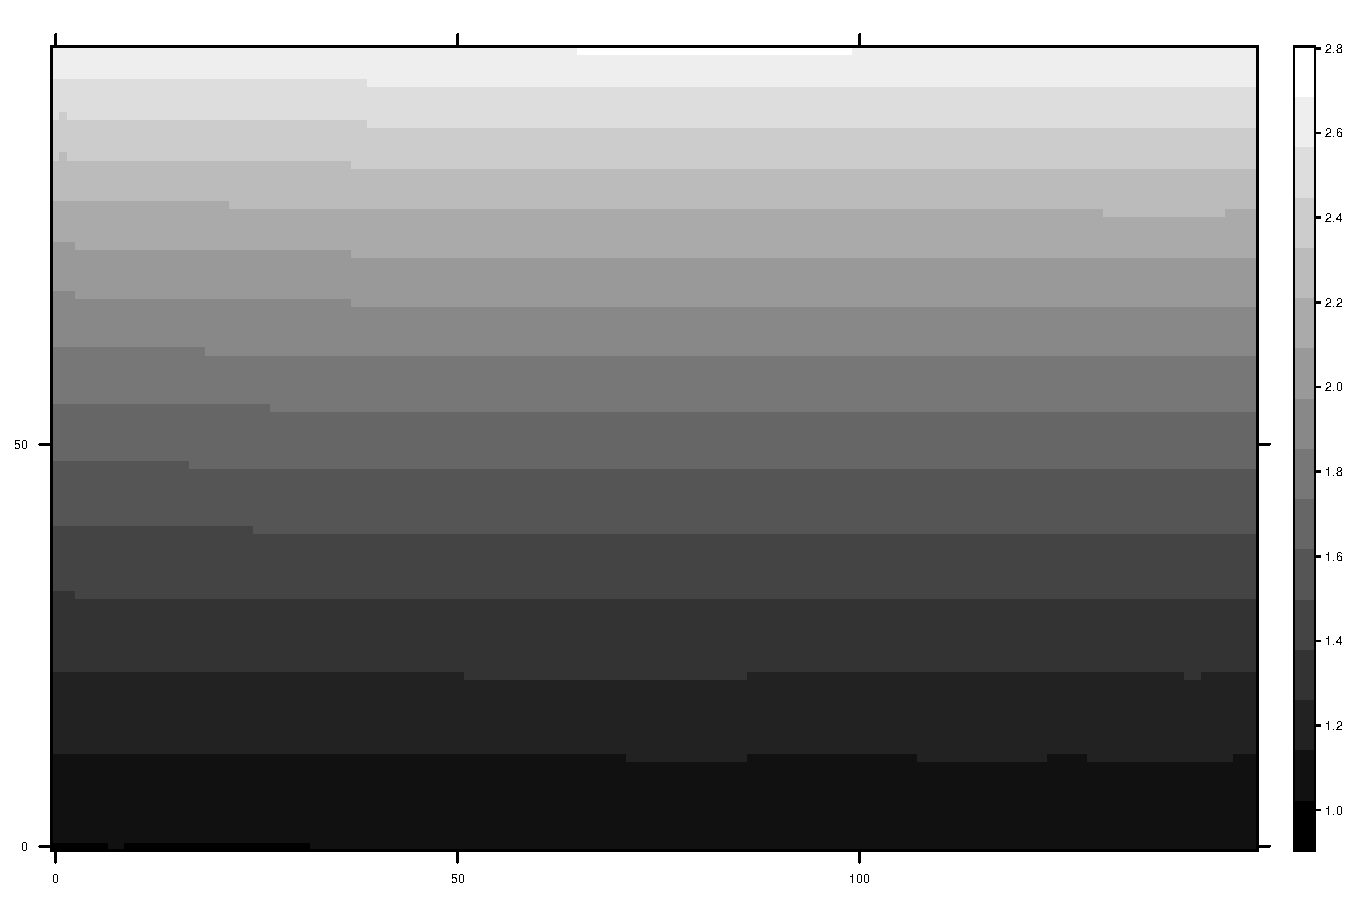
\includegraphics[width=\textwidth]{2dssa_rec}
        \caption{Восстановленный тренд.}
        \label{fig:2dssa_rec}
    \end{subfigure}
    \caption{2D-SSA пример}
\end{figure}

\conclusion
В работе рассматривался метод SSA (Singular spectrun analysis) анализа временных рядов и задача выделения аддитивных составляющих, определяемых как тренд и колебательная составляющая, из известного объекта $\mathbb{X}$, который может являться либо вещественным временным рядом, либо комплексным, либо системой временных рядов, либо двумерным изображением. В зависимости от типа объекта $\mathbb{X}$ к нему применяется либо 1D-SSA, либо CSSA, либо MSSA, либо 2D-SSA методы соответственно.

В разделе \ref{sec:1d_methods} был сделан обзор для 1D-SSA всех найденных существующих методов группировки компонент, методов выделения тренда и колебательной составляющей, и были приведены примеры статей, использующих данные методы. 

В главе \ref{sec:tau1} был исследован и доработан новый метод идентификации колебательной составляющей, идея которого была предложена ранее в моей бакалаврской работе \cite{Zhornikova2016}. Метод показал свою эффективность на модельных и реальных примерах, но не удалось придумать и теоретически обосновать универсальный метод выбора порога; зато метод обоснован для модулированных гармоник, в отличие от другого известного метода, описанного в разделе \ref{sec:1d_pgram_method}. В разделе \ref{sec:compare} оба метода были сравнены, и новый метод показал более высокую эффективность.

Из исследований, проведенных в работе для 1D-SSA методов, можно сделать следующие выводы. Для идентификации тренда существует хорошо обоснованный метод низких частот, реализуемый алгоритмом \ref{alg:freq1d}, который имеет рекомендации и обоснования для выбора параметров. Для колебательной составляющей всё еще не существует полностью обоснованного метода с рекомендациями по выбору параметров.

Многие методы автоматической идентификации для 1D-SSA были обобщены в главе \ref{sec:all_methods} для других вариантов объекта $\mathbb{X}$ и вариантов метода SSA. Для MSSA и CSSA был обобщен метод идентификации тренда и два, уже упоминавшихся, метода идентификации колебательной составляющей. Для 2D-SSA был обобщен только метод идентификации тренда. 
Возможно, для двумерного изображения также можно обобщить методы идентификации колебательной составляющей, этот вопрос не был исследован.

Два алгоритма \ref{alg:1d_pgram}, \ref{alg:1dtau_2} для 1D-SSA были реализованы на языке R, код реализации можно найти в \cite{polina_zhornikova_2018_1252476}. 
Также были реализованы все обобщенные алгоритмы из главы \ref{sec:all_methods} кроме кластерного метода группировки, их реализации тоже можно найти в \cite{polina_zhornikova_2018_1252476}.

\bibliographystyle{ugost2008}
\bibliography{biblio}

\end{document}


